\chapter{RESULTS}

\section{Model Constraints and Curation}


To make sure the \emph{in-silico} growth rate predictions are in agreement with the physiological kinetic parameters obtained from the laboratory experiments, fine adjustment on the chosen metabolic model is a requirement. Since the growth-associated maintenance (GAM) and non-growth associated maintenance (NGAM) reactions in a model play a determinant role in the simulation results, fluxes through these reactions must be constrained to a fixed value. Flux of the NGAM reaction is constrained to 0.7 mmol/gDWh\textsuperscript{-1} for aerobic model, and 0 mmol/gDWh\textsuperscript{-1} for anaerobic model simulations as calculated in the previous studies \cite{nilsson2016metabolic}. Since the GAM depends on the biomass composition defined, results of a chemostat experiment \cite{van1998effect} are used as a guide to fit simulation predictions to. The model is simulated iteratively with a range of values for the GAM and the best fit is found at the level of 31.4 mmol/gDWh\textsuperscript{-1} (Figure \ref{fig:gam_fitting}).

\begin{figure}[H]
  \begin{center}
      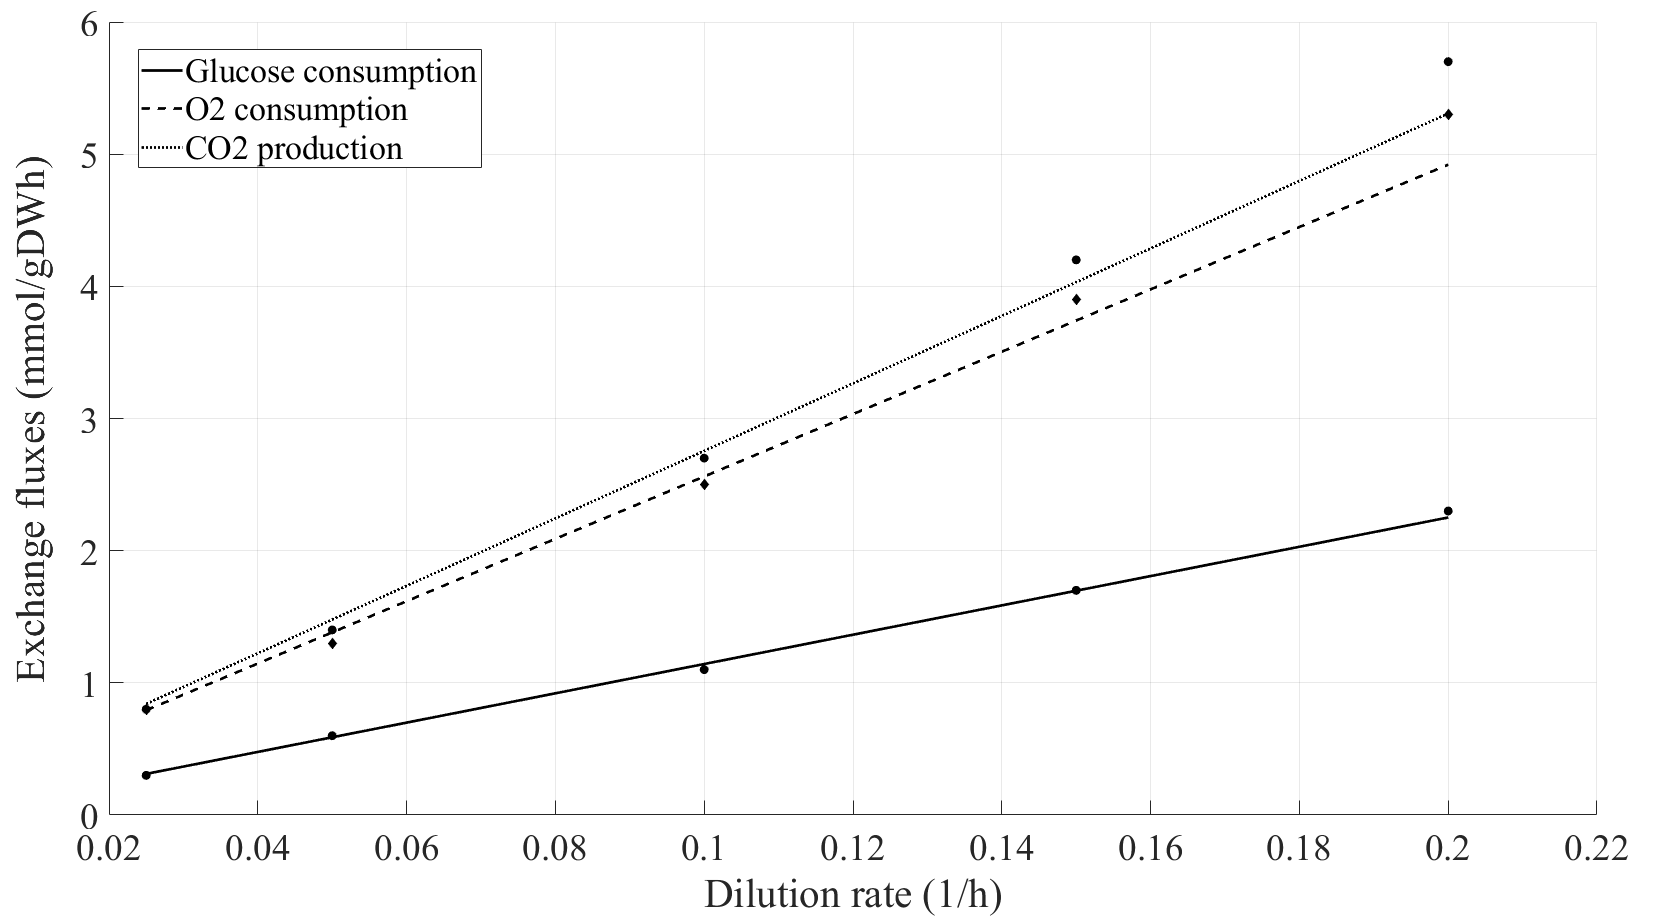
\includegraphics[width=1\columnwidth]{figures/gamfitting.png}
      \caption[The required flux for the growth associated maintenance reaction is determined by the fitting simulation results to the experimental data]{The required flux for the growth associated maintenance reaction is determined by the fitting simulation results to the experimental data. The best fit is found at 31.4 mmol/gDWh\textsuperscript{-1} and the reaction is constrained to that flux value.}
      \label{fig:gam_fitting}
  \end{center}
\end{figure}

Average enzyme saturation value is set to 50\% where the lowest error rate is obtained as a fraction to biomass (Figure \ref{fig:sigma_fitting}). By constraining the total enzyme mass, the metabolic model became able to show overflow metabolism without any other constaint applied.

\begin{figure}[H]
  \begin{center}
    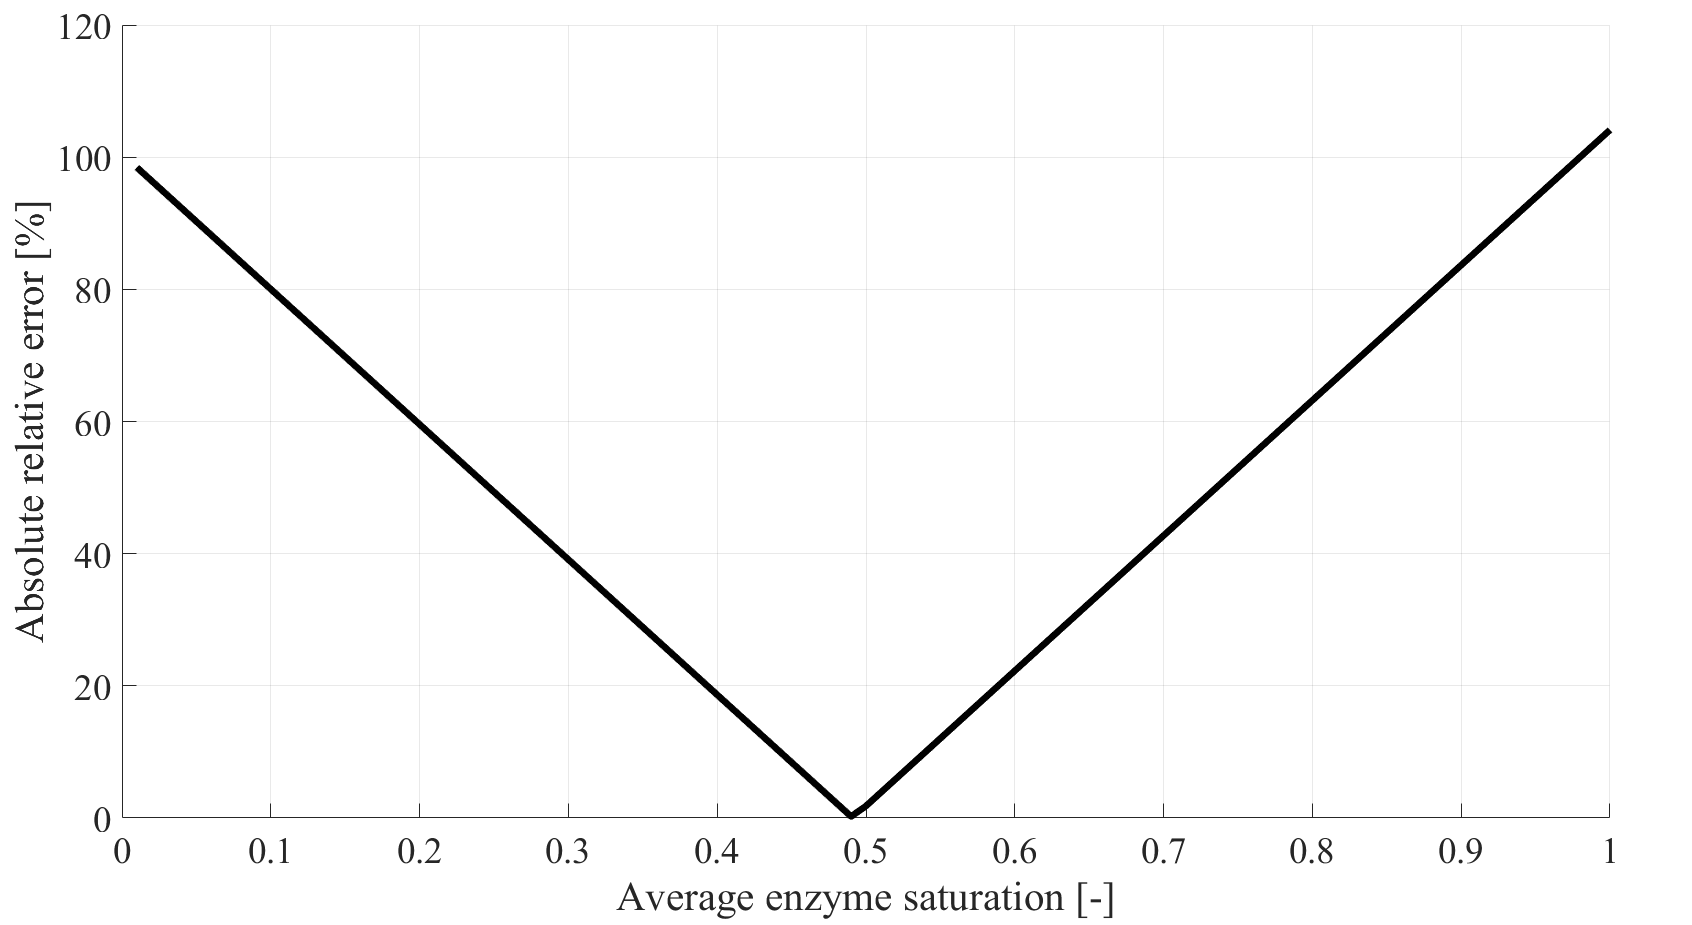
\includegraphics[width=1\columnwidth]{figures/sigmafitting.png}
    \caption[Average enzyme saturation factor for the GECKO method is determined by the iterative simulations for the lowest absolute relative error to the experimantal data]{Average enzyme saturation factor for the GECKO method is determined by the iterative simulations for the lowest absolute relative error to the experimantal data. The value is set to 50\% where the lowest error rate is obtained.}
    \label{fig:sigma_fitting}
  \end{center}
\end{figure}

To prevent over-constraining the model with the enzyme kinetics, the most limiting proteins in the model are found based on their sensitivity on the objective function, i.e. growth. The $k_{cat}$ values for the the limiting enzymes are updated with the maximum available values from BRENDA\cite{jeske2019brenda} database by automated iterations until the simulation results for the growth rate agrees with the experimental growth rate. These alterations for enzymes with their objective control coefficients can be found in the Table \ref{table:gecko_iterations}.

\begin{table}[H]
  \begin{center}
  \caption[Iterations on the network to find the top limiting proteins by their objective control coefficients (cc), i.e. sensitivities on the growth, with previous and updated $k_{cat}$ values and error improvements]{Iterations on the network to find the top limiting proteins by their objective control coefficients (cc), i.e. sensitivities on the growth, with previous and updated $k_{cat}$ values and error improvements. }
  \vskip0.5\baselineskip
  \begin{tabular}{ccp{5cm}cccc}
     \hline
    \textbf{\#} & \textbf{Protein} & \textbf{Reaction Name} & \textbf{prev $k_{cat}$} & \textbf{new $k_{cat}$} & \textbf{CC} & \textbf{Err\%}  \\
      \hline
      1 & P38604 & lanosterol synthase & 0.002 & 4.076 & 0.937 & -42.6 \\ \hline
      2 & P38972 & 5'-phosphoribosylformyl \newline glycinamidine synthetase & 0.05 & 5.07 & 0.244 & -28.7 \\   \hline
      3 & P00931 & tryptophan synthase \newline (indoleglycerol phosphate) & 0.022 & 775.75 & 0.129 & -19.4 \\   \hline
      4 & P48445 & acetyl-CoA carboxylase & 1.23 & 450000 & 0.065 & -14.2 \\   \hline
      5 & P05694 & methionine synthase & 0.33 & 3.5 & 0.050 & -10.3 \\   \hline
      6 & P39006 & PS decarboxylase \newline (1-16:1, 2-16:1) & 0.053 & 366.667 & 0.043 & -6.4 \\   \hline
  \end{tabular}
  \label{table:gecko_iterations}
  \end{center}
\end{table}


\vspace{-0.5cm}
\section{Differential Expression Analysis and Integration}

The obtained expression datasets were quantile-normalized for their own experiments. Three replicates for both reference and the evolved strains for each experiment (exception with the ethanol-b8 strain which has two replicates) is used for the differential expression analysis. The distribution across normalized gene expression levels across each experiment can be seen in the Figure \ref{fig:expr_boxplot}. No further normalization applied to prevent introducing errors and datasets are used as obtained from the database.

\begin{figure}[H]
  \begin{center}
  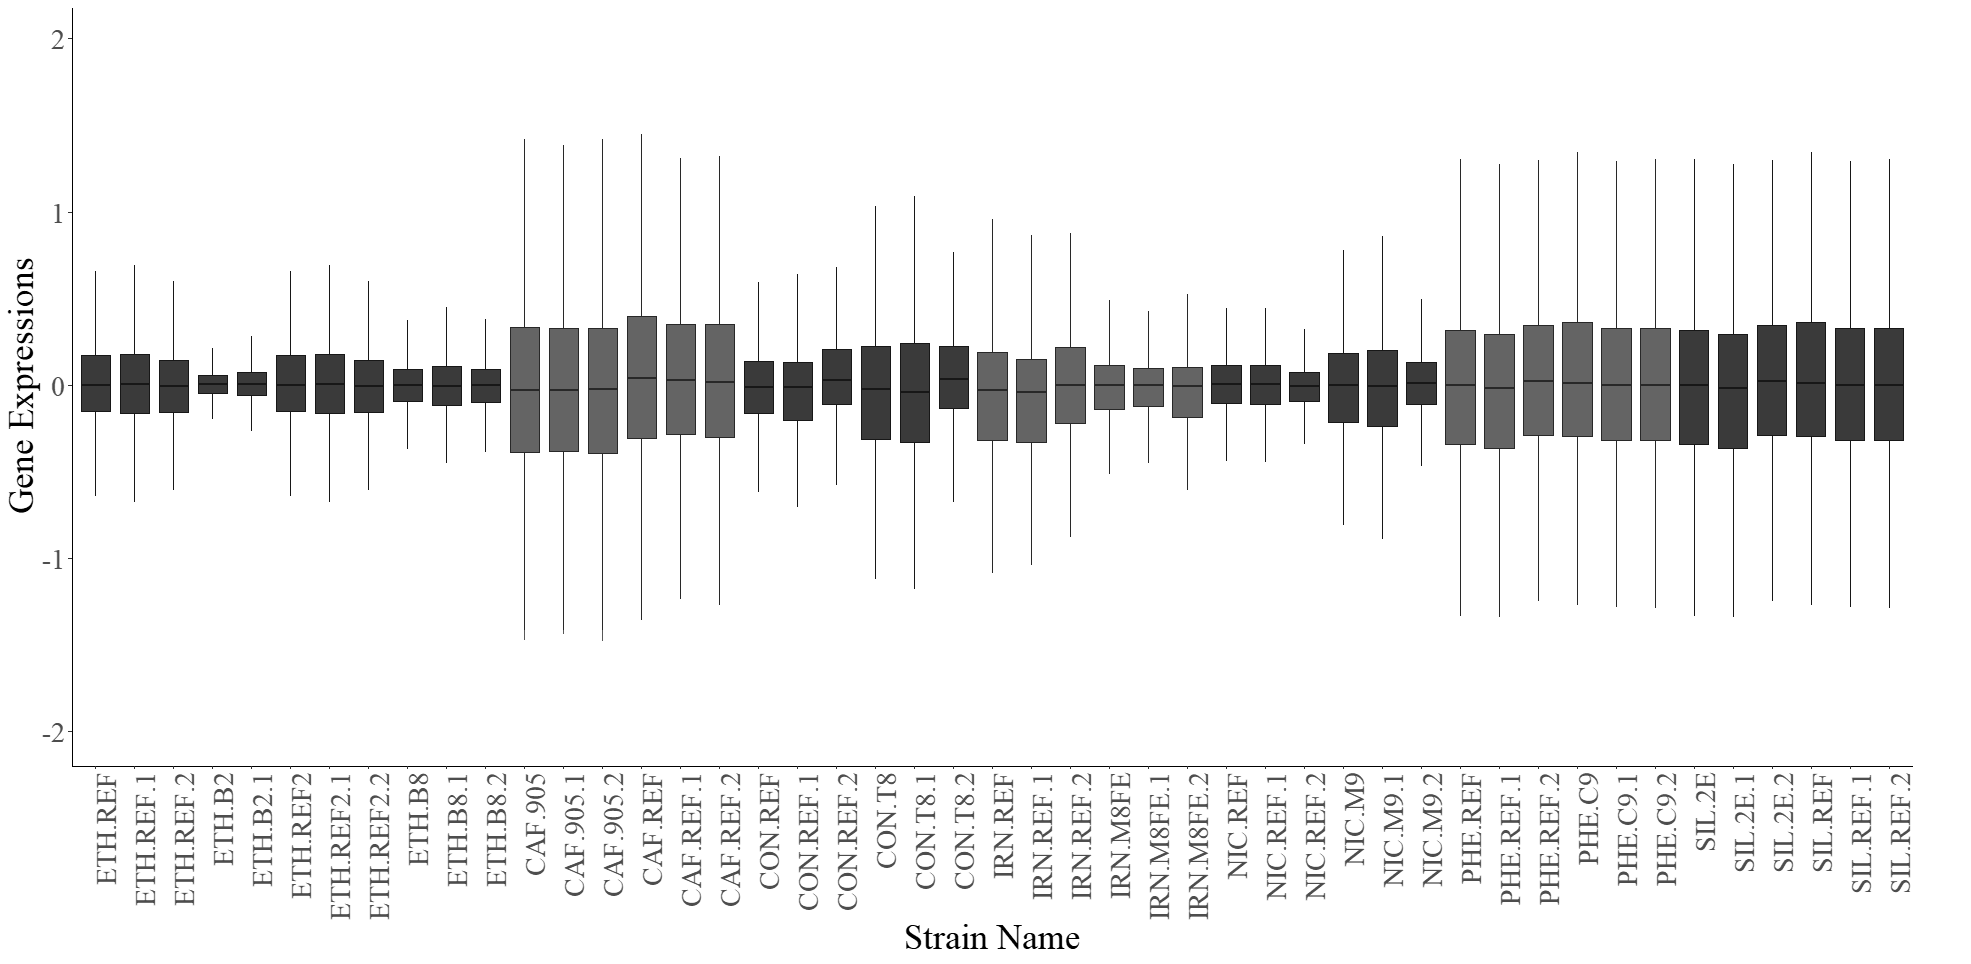
\includegraphics[width=1\columnwidth]{figures/expr_boxplots.png}
  \caption[Boxplots of the normalized gene expression levels]{Boxplots of the normalized gene expression levels obtained from Gene Expression Omnibus. Quantile normalization performance is indicated by the medians (black horizontal lines) that are almost at the same level with their reference reads.}
  \label{fig:expr_boxplot}
  \end{center}
\end{figure}

A statistical threshold (p $<$ 0.05) for the differential analysis of the normalized gene expression levels detected a total of 1606 genes in ethanol-b2, 2947 genes in ethanol-b8, 4743 genes in caffeine, 2267 genes in coniferylaldehyde, 3448 genes in iron, 152 genes in nickel, 4796 genes in phenylethanol, and 4796 genes in silver resistant strains differentially expressed. Commonly upregulated and downregulated genes frequencies across all strains can be found in the Figure \ref{fig:intersections_by_degree}.



\begin{figure}[H]
  \begin{center}
  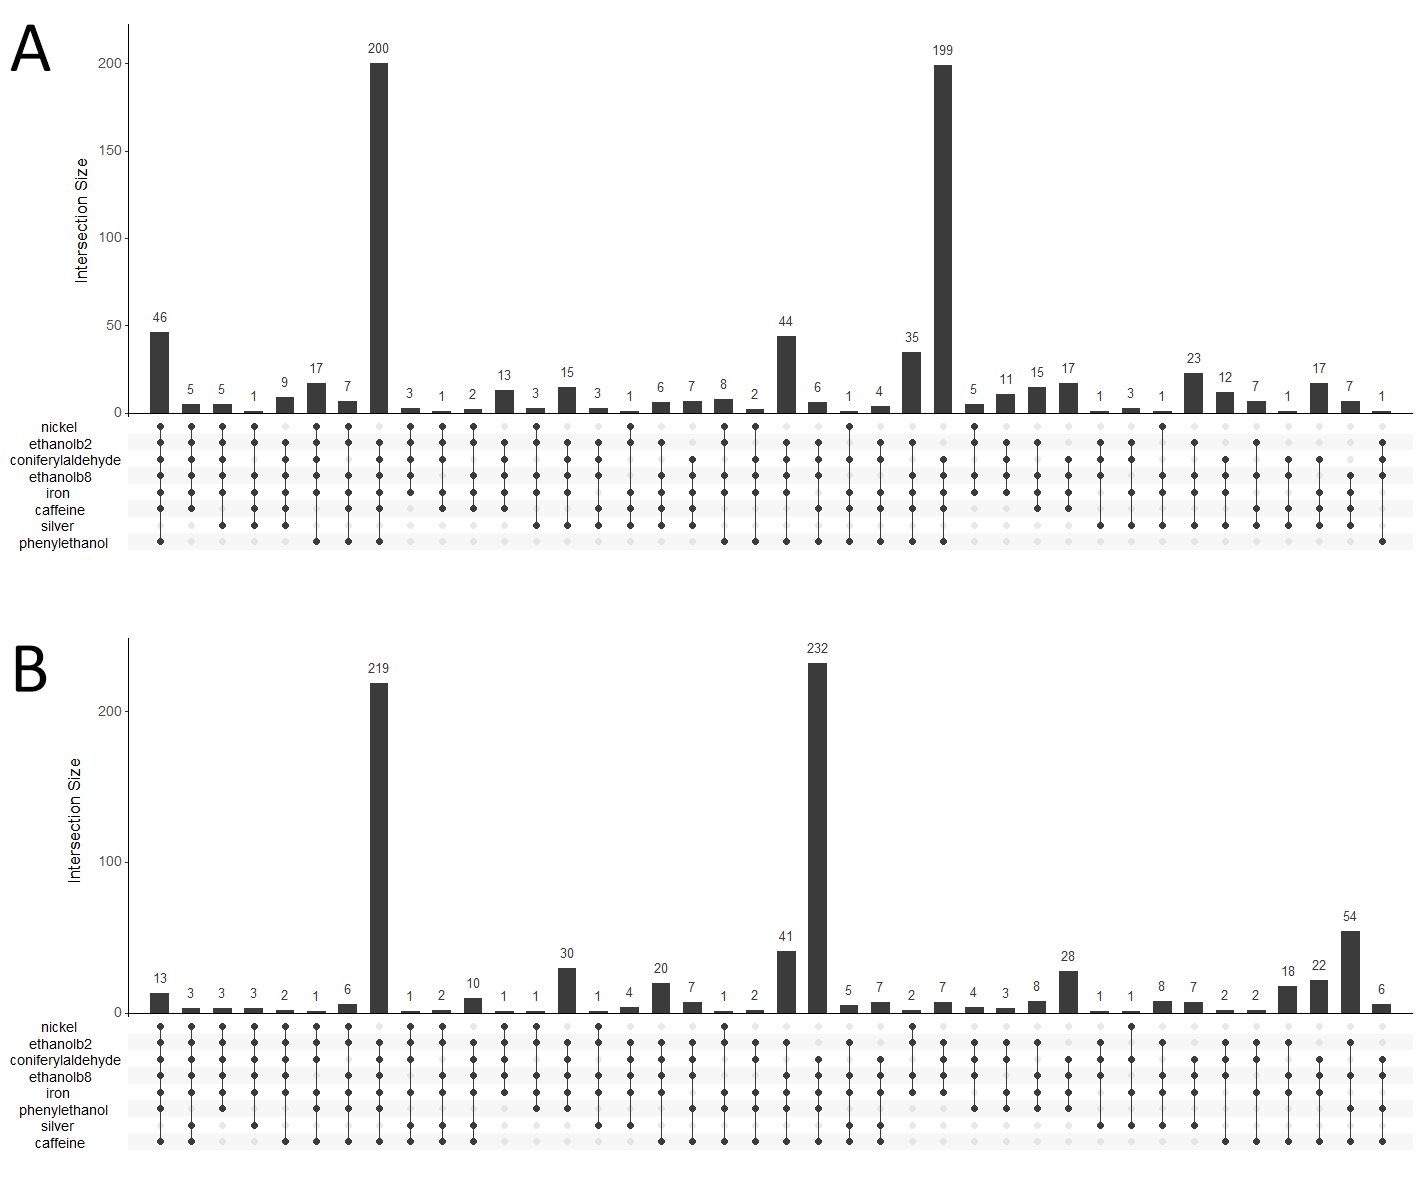
\includegraphics[width=1\columnwidth]{figures/intersections_by_degree.png}
  \caption[UpSet plot showing the number of common genes that are differentially expressed significantly]{UpSet plot showing the number of common genes that are differentially expressed significantly (p $<$ 0.05) across evolved strains. Connected black circles in the below panel's matrix represents a certain intersection between experiment strains, and the number of genes in that intersection are shown in the top bar graphs. Differentially expressed genes are plotted seperately for (A) upregulated genes, and (B) downregulated genes.}
  \label{fig:intersections_by_degree}
  \end{center}
\end{figure}

Despite the high number of differentially expressed genes in the silver resistant strain, the intersection with the most number of strains discluded it. There were not any common differentially expresssed genes considering all strains. The most common genes (as shown in the first bars in the UpSet plot) are reported in Table \ref{table:common_genes}.

\begin{table}[H]
\small
\vskip\baselineskip
  \begin{center}
  \caption[Common upregulated and downregulated genes]{The common upregulated and downregulated genes within ethanolb2, ethanolb8, caffeine, coniferylaldehyde, iron, nickel and phenylethanol resistant strains.}
    \vspace{5mm}
  \begin{tabular}{|p{4cm}|p{10cm}|}
     \hline
    \textbf{Upregulated Genes} & \textbf{Downregulated Genes}  \\
      \hline
      YDR075W, YDR492W, YGR239C, YIL118W, YLR215C, YML005W, YML125C, YNL024C, YNL188W, YNR044W, YOL002C, YOR107W, YPR052C & YBL015W, YBR132C, YBR285W, YBR299W, YCR068W, YDL238C, YDR055W, YER033C, YGL146C, YGL250W, YGR023W, YGR149W, YGR161C, YGR288W, YGR289C, YGR292W, YIL097W, YIR017C, YJL042W, YJL053W, YJL082W, YJL132W, YLR092W, YLR176C, YLR240W, YLR446W, YMR052C-A, YMR053C, YMR081C, YMR103C, YMR104C, YMR105C, YMR160W, YMR194C-A, YMR258C, YMR291W, YNL093W, YNL277W, YNR001C, YOL117W, YOR027W, YOR132W, YOR178C, YOR230W, YPR079W, YPR154W \\ \hline
  \end{tabular}

  \label{table:common_genes}
  \end{center}
\end{table}



The log2(fold-change) values of differentially expressed genes and their frequencies are plotted for each experiment in Figure \ref{fig:expr_frequencies_before}. Although the high number of differentially expressed genes are collected, due to the limited reaction number in the genome-scale metabolic models, only a part of obtained fold-change expression values were able to be integrated. Because of the limitations in the model, no further cutoff considered for the fold change values.

\begin{figure}[H]
  \begin{center}
  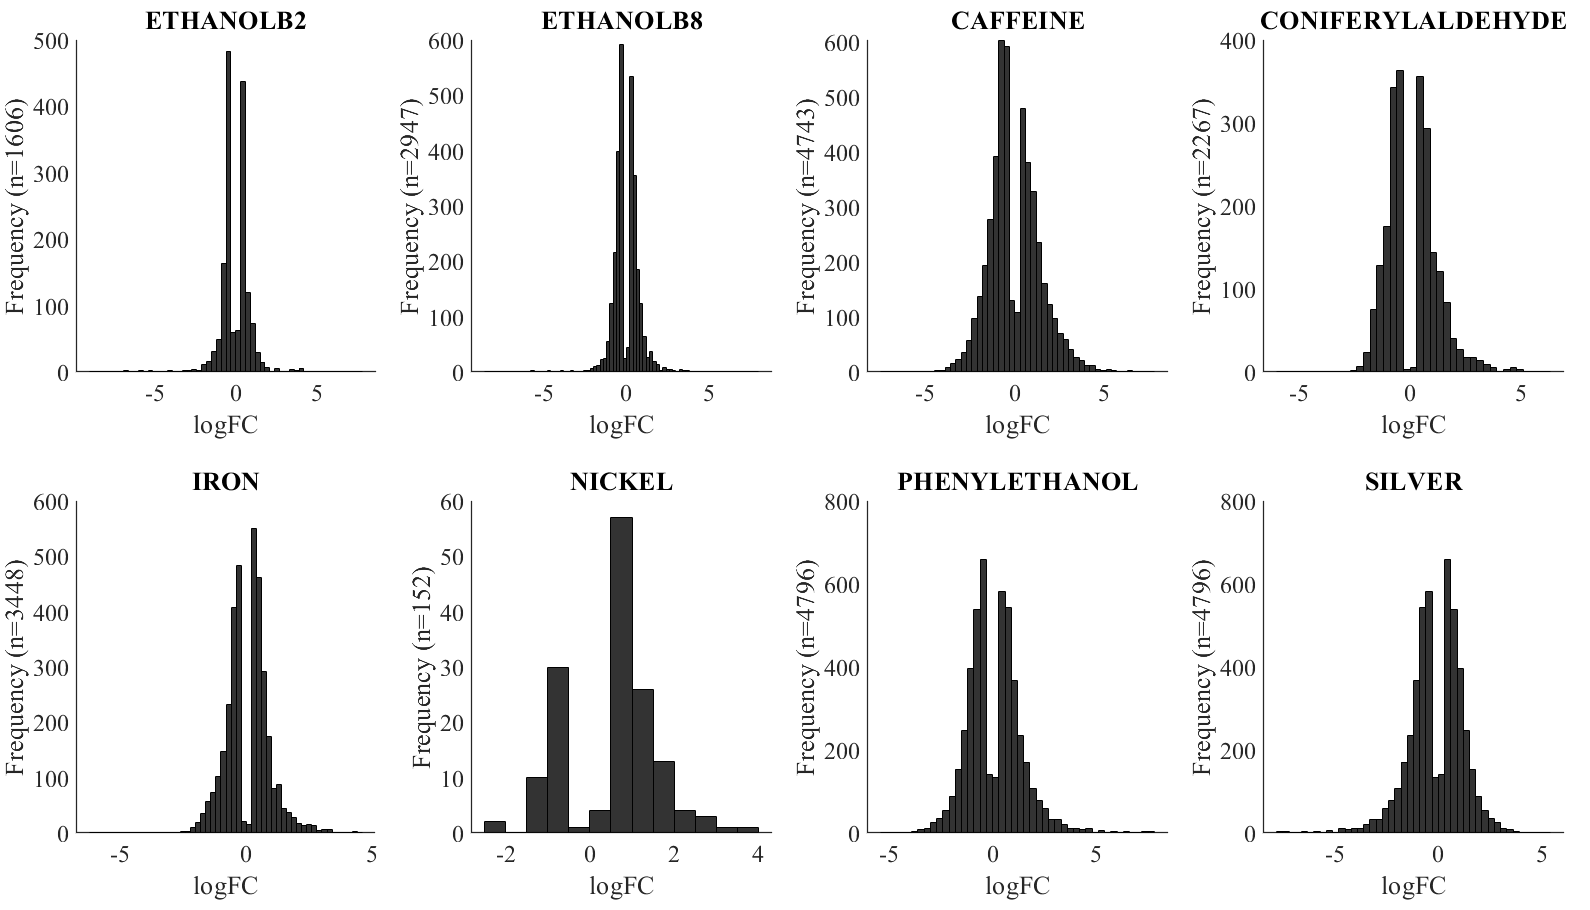
\includegraphics[width=1\columnwidth]{figures/expr_frequencies_before.png}
  \caption[Frequencies of the differentially expressed genes after the gene expression analysis]{Frequencies of the differentially expressed genes after the gene expression analysis.}
  \label{fig:expr_frequencies_before}
  \end{center}
\end{figure}

Total of 277 genes in ethanol-b2, 464 genes in ethanol-b8, 783 genes in caffeine, 374 genes in coniferylaldehyde, 552 genes in iron, 28 genes in nickel, 759 genes in phenylethanol and 759 genes in silver resistant strains were integrated into the metabolic model to generate strain-specific models (Figure \ref{fig:expr_frequencies_after}).

\begin{figure}[H]
  \begin{center}
  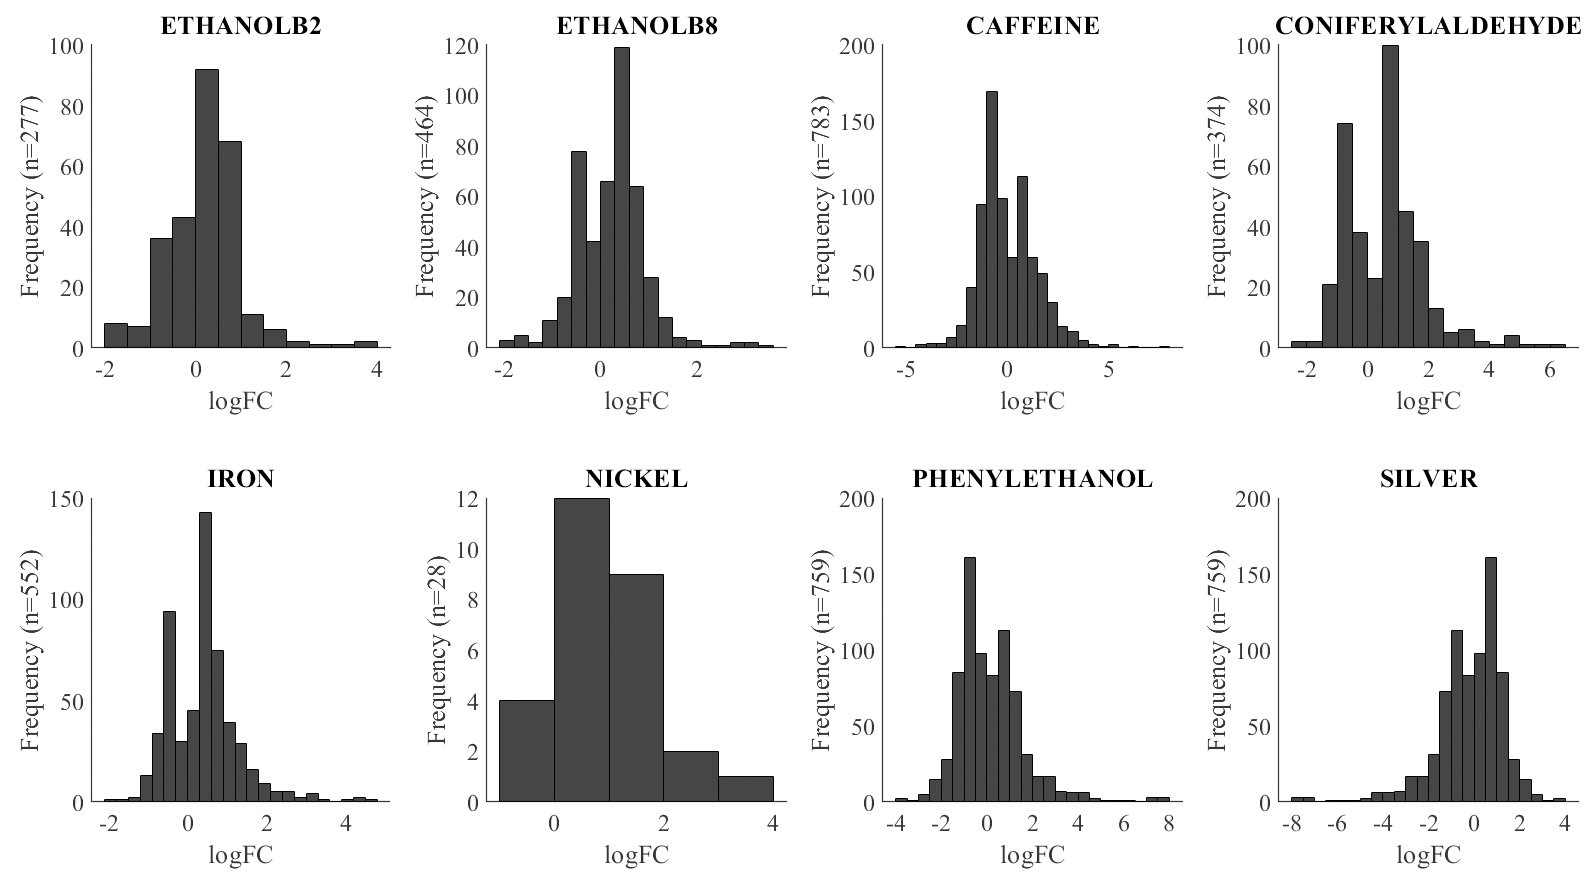
\includegraphics[width=1\columnwidth]{figures/expr_frequencies_after.png}
  \caption[Frequencies of the differentially expressed genes that are integrated into the metabolic model]{Frequencies of the differentially expressed genes that are integrated into the metabolic model.}
  \label{fig:expr_frequencies_after}
  \end{center}
\end{figure}

In comparison, 14.13\% of genes in ethanol-b2, 15.74\% of genes in ethanol-b8, 16.51\% of genes in caffeine	16.50\% of genes in coniferylaldehyde, 16.01\% of genes in iron, 18.42\% of genes	in nickel, 15.83\% of genes in phenylethanol and 15.83\%  of genes in silver resistant strains were found in the metabolic model and they are integrated.

In order to validate the expression data integration method, fluxes for each enzyme (i.e. protein flux from protein pool to reaction for each protein) is predicted by flux balance analysis on all the strain models and on the wild-type model (wild-type here is referred as the metabolic model without expression data integrated). Flux ratios between wild-type and evolved models are calculated, and linear regression analysis is fitted after elimination of the outliers by the generalized extreme studentized deviate test to compare the flux-changes with the protein fold-changes from the expression data. Results confirm a good correlation between simulations and protein fold-change values (Figure \ref{fig:expr_linear_regressions}).

\begin{figure}[H]
  \begin{center}
  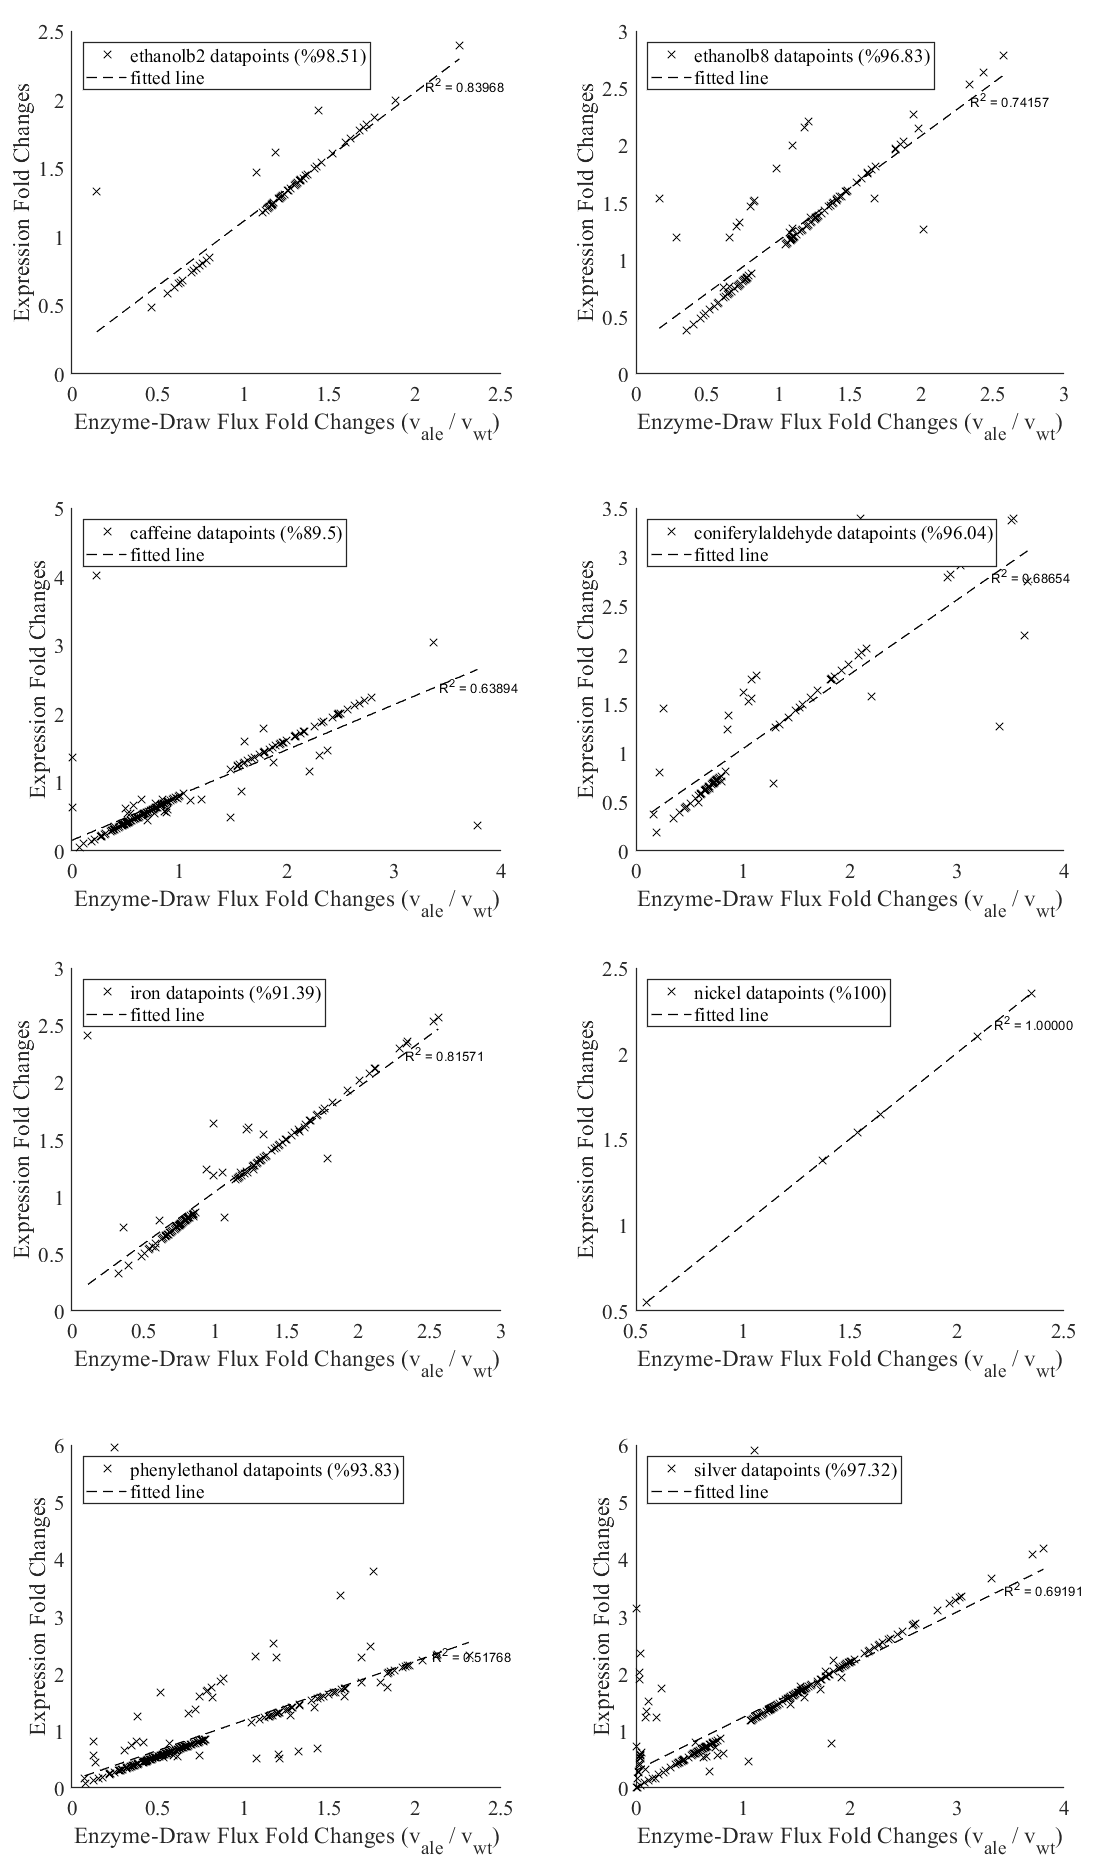
\includegraphics[width=0.8\columnwidth]{figures/expr_linear_regressions.png}
  \caption[Linear regression analyses of the fold-changes]{Linear regression analyses of the differential expression fold-changes obtained from microarray studies and the enzyme-draw flux fold-changes obtained from flux balance analysis simulations of corresponding proteins.}
  \label{fig:expr_linear_regressions}
  \end{center}
\end{figure}


\section{Flux Balance Analysis Simulations}

The metabolic model is first simulated without the integration of the expression data (this model will be referred as wild-type model). Since the model is already enzymatically constrained, the only additional constraint required is the total amout of enzymes available in the enzyme pool. All the lower bounds for reactions were set to 0, and the upper bounds were set to 1000, except for the enzyme pool reaction. By doing that, the model was set free to be able to allocate enzymes as the reactions require. Flux rates of several exchange reactions as a function of growth rate are plotted in Figure \ref{fig:wt_crabtree}.

A behavioral change is observed around the time when growth rate is approximately 0.3 h\textsuperscript{-1}. Since the model is simulated under fully areobic conditions (no constraints applied) and produces ethanol, this behavior can be explained by the Crabtree effect, where the yeast metabolism switches to perform both respiration and fermentation at the same time at a critical specific growth rate.

\begin{figure}[H]
  \begin{center}
  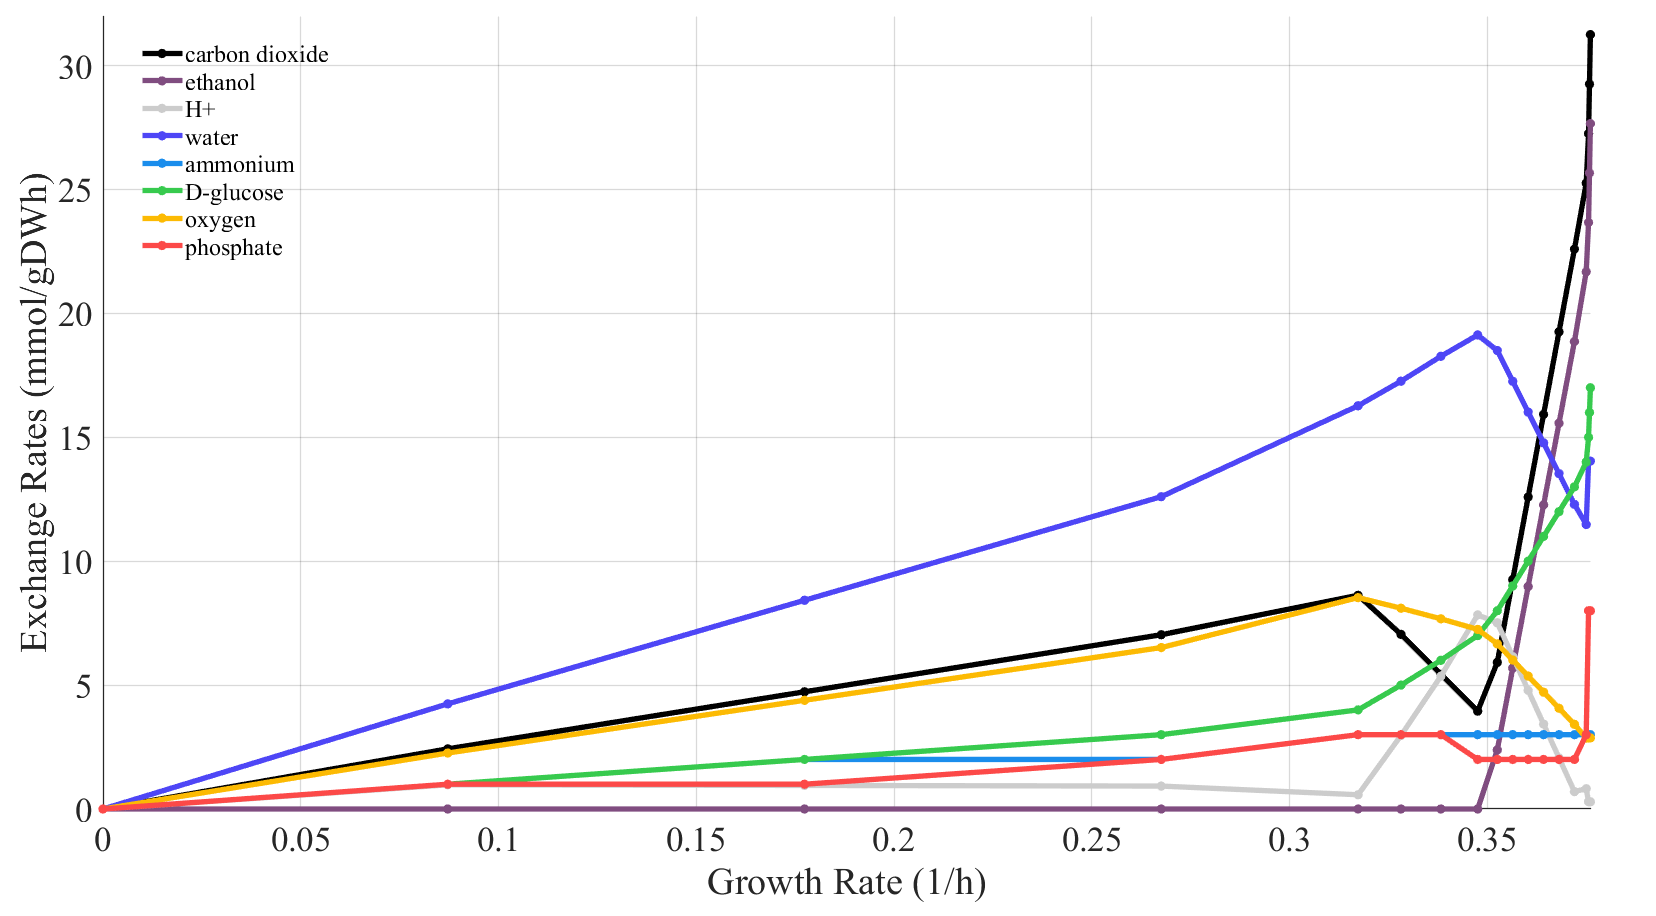
\includegraphics[width=1\columnwidth]{figures/wt_crabtree.png}
  \caption[Metabolic model shows the overflow metabolism]{Metabolic model shows the overflow metabolism (crabtree effect) under fully aerobic conditions.}
  \label{fig:wt_crabtree}
  \end{center}
\end{figure}

Robustness analysis is performed on the wild-type model for the growth rate with the varying levels of glucose uptake, oxygen uptake, acetate secretion and ethanol secretion rates (Figure \ref{fig:wt_robustness}). Unlike the traditional metabolic models, enzymatically constrained model showed non-linear graphs.

\begin{figure}[H]
  \begin{center}
  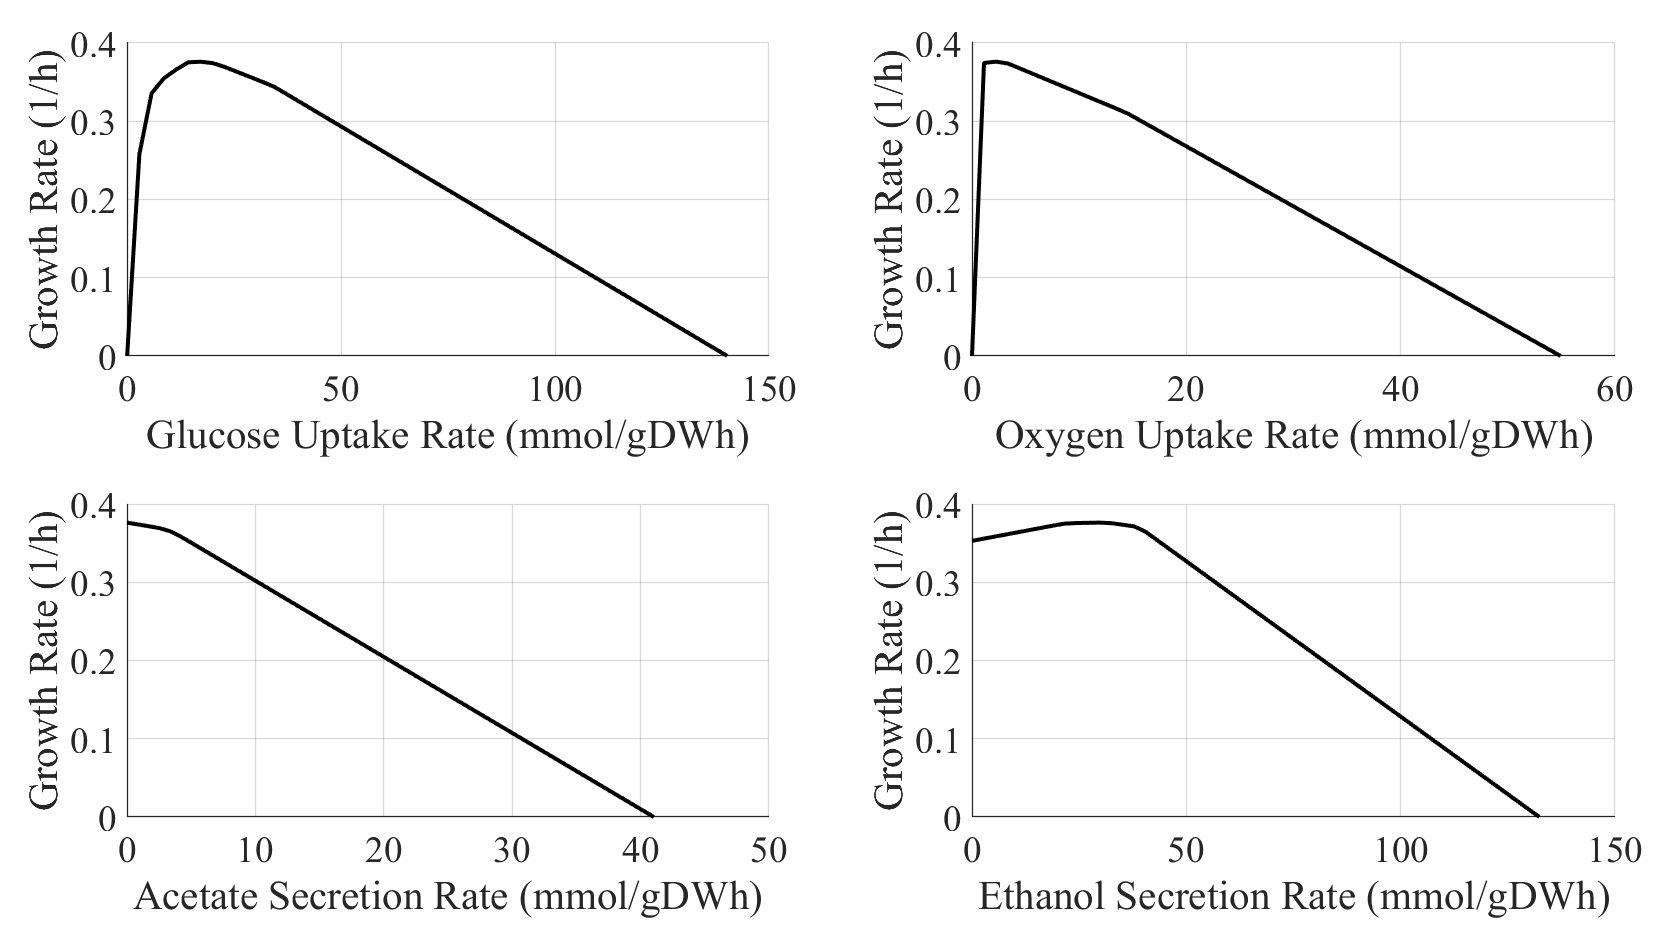
\includegraphics[width=1\columnwidth]{figures/wt_robustness.png}
  \caption[Robustness analyses on the glucose uptake, oxygen uptake, acetate secretion and ethanol secretion rates]{Robustness analyses on the glucose uptake, oxygen uptake, acetate secretion and ethanol secretion rates.}
  \label{fig:wt_robustness}
  \end{center}
\end{figure}

After the validation of the wild-type model, all models for strains are simulated for the growth rates as a function of iteratively increasing glucose uptake rates (Figure \ref{fig:growth_glucose_ales}). Models were able to grow up to the point where the protein accesibility becomes a limiting factor. It has been found that the evolution models except for the caffeine tolerant model show similar patterns on the points where the enzymes become limiting (break points in the lines). Caffeine tolerant model shows different pattern in a way that it can consume more glucose to reach higher growth rates compared to others. Also it must be noted that while only caffeine and coniferylaldehyde tolerant models can grow at higher rates than wild-type model, ethanol, iron, nickel, phenylethanol and silver models can grow at lower maximum rates. The maximum growth rates and corresponding glucose uptake rates for each model are summarized in the Table \ref{table:growth_glucose_table}.

\begin{figure}[H]
  \begin{center}
  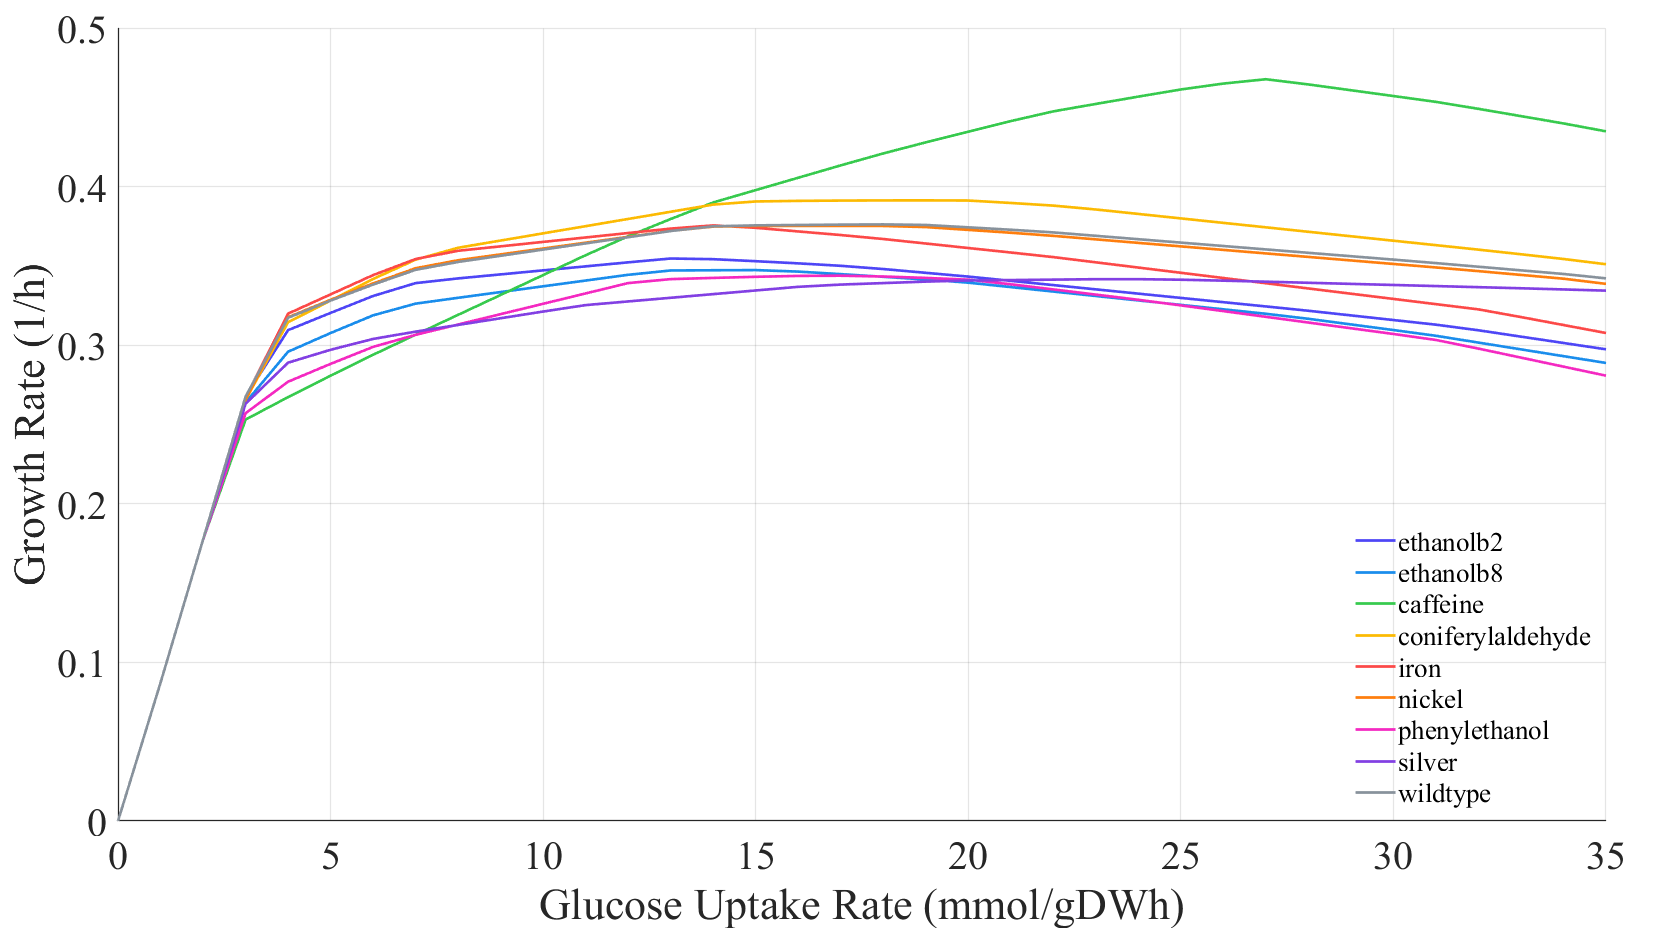
\includegraphics[width=1\columnwidth]{figures/growth_glucose_ales.png}
  \caption[Growth rates as a function of iteratively increasing glucose uptake rates]{Growth rates as a function of iteratively increasing glucose uptake rates.}
  \label{fig:growth_glucose_ales}
  \end{center}
  \end{figure}
\vspace{-1.0cm}



\begin{table}[H]
\small
\vskip\baselineskip
  \begin{center}
  \caption[Maximum growth rates obtained from flux balance analysis simulations for each strain and their maximum glucose uptake rates (GUR) required for the growth]{Maximum growth rates obtained from flux balance analysis simulations for each strain and their maximum glucose uptake rates (GUR) required for the growth.}
    \vspace{5mm}
  \begin{tabular}{|c|c|c|}
     \hline
    \textbf{Experiment} & \textbf{Growth Rate (1/h)} & \textbf{GUR (mmol/gDWh)} \\
      \hline
      ethanolb2           & 0.35466                    & 14                                       \\ \hline
      ethanolb8           & 0.34736                    & 16                                       \\ \hline
      caffeine            & 0.46769                    & 28                                       \\ \hline
      coniferylaldehyde   & 0.39132                    & 20                                       \\ \hline
      iron                & 0.37554                    & 15                                       \\ \hline
      nickel              & 0.37523                    & 18                                       \\ \hline
      phenylethanol       & 0.34382                    & 18                                       \\ \hline
      silver              & 0.34163                    & 25                                       \\ \hline
      wildtype            & 0.37618                    & 19                                       \\ \hline
  \end{tabular}
  \label{table:growth_glucose_table}
  \end{center}
\end{table}

Phenotype phase planes are obtained through double robustness analysis to see the effect of oxygen on growth while the systems are fed with the gradually increasing glucose levels. Contour plots showing different regions can be seen in the Figure \ref{fig:robustness_glu_oxy}. Minimum and maximum values of oxygen uptake rates (y-axis) and glucose uptake rates (x-axis) are kept same in all 8 plots to ne able to observe growth capacity of different resistant models clearly.

\begin{figure}[H]
  \begin{center}
  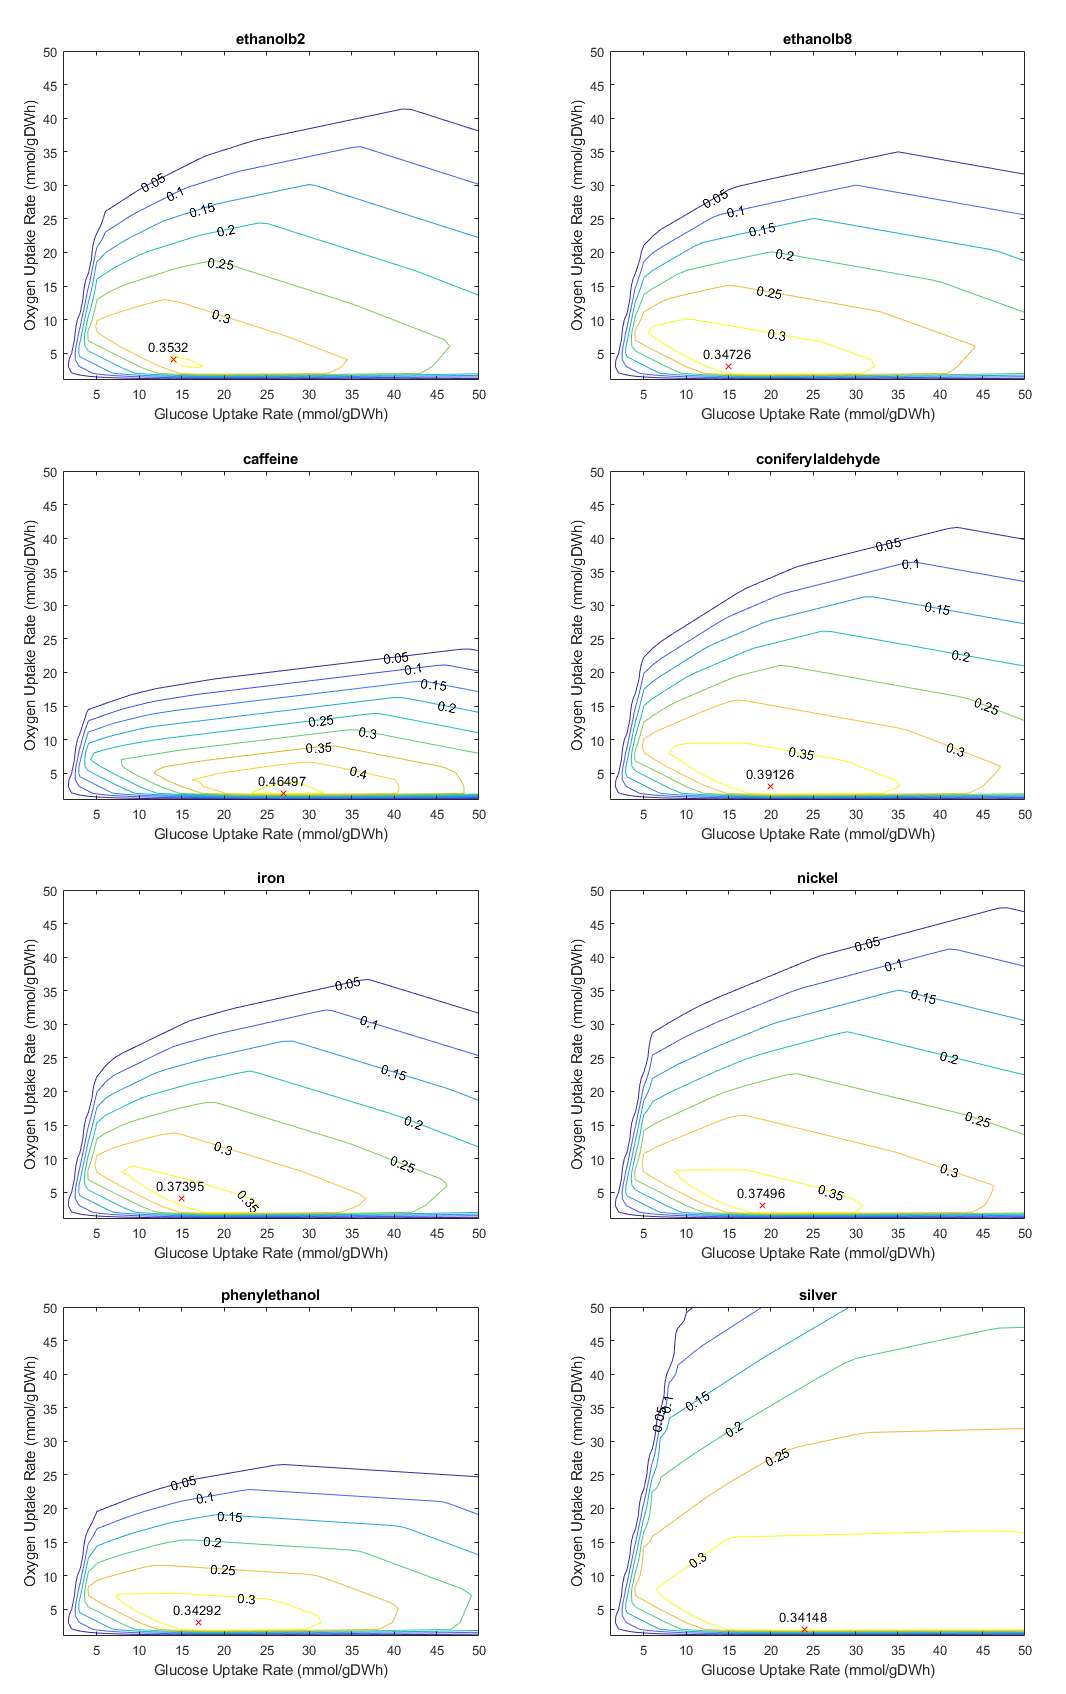
\includegraphics[width=0.85\columnwidth]{figures/robustness_glu_oxy.png}
  \caption[The glucose uptake rate (mmol/gDWh) versus oxygen uptake rate (mmol/gDWh) phenotype phase planes show the cellular growth rate as colored contours for each adapted model simulations]{The glucose uptake rate (mmol/gDWh) versus oxygen uptake rate (mmol/gDWh) phenotype phase planes show the cellular growth rate as colored contours for each adapted model simulations. Maximum points are shown as red cross.}
  \label{fig:robustness_glu_oxy}
  \end{center}
  \end{figure}
\vspace{-1.0cm}

 Since the total area of the plots are the same (x-axis and y-axis ranges), available growth of models can be compared. On the low glucose uptake rates, growth rate countours have steep slopes for all models. They reach the growth rate of 0.3 h\textsuperscript{-1} when the glucose uptake rates are varying between 5-10 mmol/gDWh. Despite having the highest possible growth rate at 0.46497 h\textsuperscript{-1}, caffeine resistant model has the smallest area to produce biomass. It cannot grow if the oxygen uptake rate is higher than 25 mmol/gDWh, making it sensitive hyperoxic conditions. Silver resistant model on the otherhand is able to grow at high rates of both oxygen and glucose uptake rates.

In order to characterize the differentiating reactions in the flux balance analysis solution vectors, cumulative flux vectors of each experiment are plotted (Figure \ref{fig:cumflux_free}). It must be remembered that at this point, the only constraint applied to the models is the level of enzymes available in the enzyme pool. In other words, the models are able to allocate enzymes as the reactions require while all other sources (carbon, nitrogen, etc.) are unlimited. Standart deviations for each reaction between strains are calculated to find most diverging points and plotted as a bar graph.

\begin{figure}[H]
  \begin{center}
  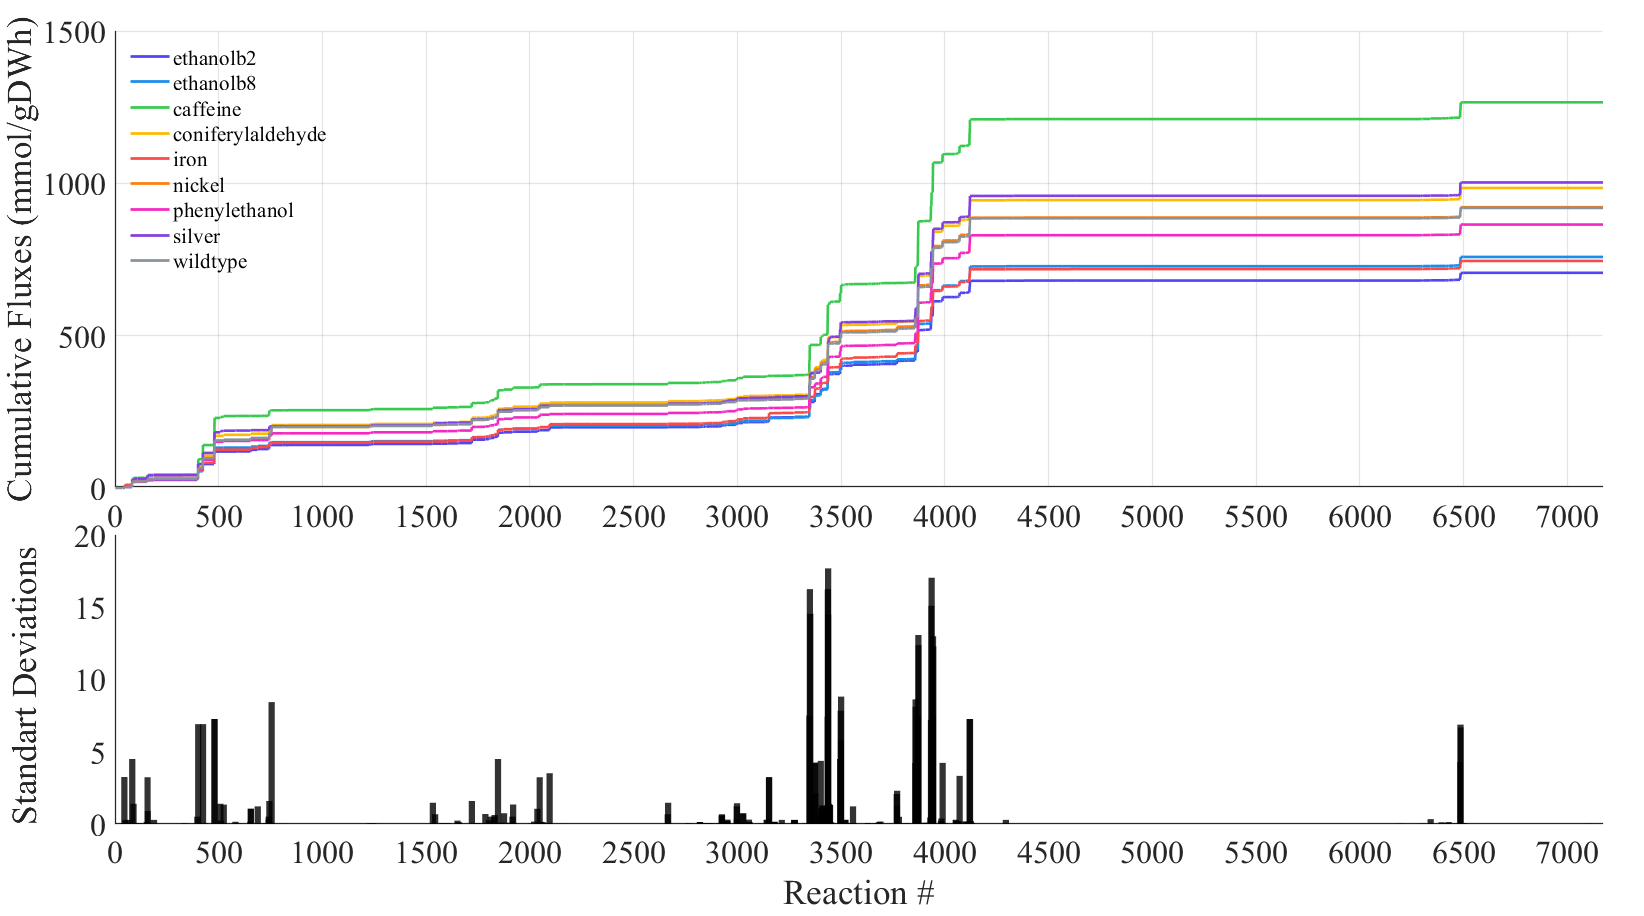
\includegraphics[width=1\columnwidth]{figures/cumflux_free.png}
  \caption[Cumulative flux vectors of each model simulations under unlimited glucose uptake constraints and the standart deviations of reactions across each adaptation]{Cumulative flux vectors of each model simulations under unlimited glucose uptake constraints and the standart deviations of reactions across each adaptation.}
  \label{fig:cumflux_free}
  \end{center}
\end{figure}

Reactions with the standart deviation values more than 10 mmol/gDWh are listed in Table \ref{table:cumulative_free_stds}. The same reactions with different numbers in their names use different enzymes. For example, glyceraldehyde-3-phosphate dehydrogenase (GADPH) reaction can be carried out in the presence of YGR192C or YJL052W or YJR009C genes' proteins, in other words, TDH1 or TDH2 or TDH3 isozymes. Therefore there are No1, No2 and No3 versions of the same reaction, using different enzymes. It must be noted that these multiple reactions carried out with isozymes in the metabolic model may not mean a significant difference if the enzymes do not catalyze any other reaction. This means that the chosen isozyme may not matter mathematically if the flux value across the isozyme reactions are the same.

\begin{table}[H]
\caption[The most divergent reactions according to their standart deviations across all strains and their flux values in mmol/gDWh.]{The most divergent reactions according to their standart deviations across all strains and their flux values in mmol/gDWh.}
\begin{center}
  \setlength{\tabcolsep}{4pt}
  \resizebox{\textwidth}{!}{
  \begin{tabular}{cclcccccccccc}
\textbf{Rank} & \textbf{Genes} & \textbf{Reaction Nams}                            & \textbf{ethanolb2} & \textbf{ethanolb8} & \textbf{caffeine} & \textbf{coniferylaldehyde} & \textbf{iron} & \textbf{nickel} & \textbf{phenylethanol} & \textbf{silver} & \textbf{wildtype} & \textbf{std} \\ \hline
1             & YJL052W        & glyceraldehyde-3-phosphate  dehydrogenase   (No2) & 24.13              & 0                  & 0                 & 36.82                      & 0             & 32.79           & 0                      & 37.4            & 32.87             & 17.69        \\
2             & YLR134W        & pyruvate decarboxylase (No3)                      & 0                  & 0                  & 44.31             & 0                          & 22.11         & 0               & 30.08                  & 0               & 0                 & 17.04        \\
3             & YGR192C        & glyceraldehyde-3-phosphate  dehydrogenase   (No1) & 0                  & 0                  & 48.77             & 0                          & 0             & 0               & 0                      & 0               & 0                 & 16.26        \\
4             & YGR254W        & enolase (No2)                                     & 23.84              & 0                  & 48.77             & 36.5                       & 25.04         & 32.49           & 32.46                  & 0               & 32.56             & 16.25        \\
5             & YLR044C        & pyruvate decarboxylase (No2)                      & 20.94              & 25.19              & 0                 & 33.69                      & 0             & 29.42           & 0                      & 35.33           & 29.49             & 15.1         \\
6             & YMR323W        & enolase (No4)                                     & 0                  & 28.03              & 0                 & 0                          & 0             & 0               & 0                      & 37.13           & 0                 & 14.55        \\
7             & YJR009C        & glyceraldehyde-3-phosphate  dehydrogenase   (No3) & 0                  & 28.31              & 0                 & 0                          & 25.34         & 0               & 32.74                  & 0               & 0                 & 14.52        \\
8             & YOR283W        & phosphoglycerate mutase (No1)                     & 23.84              & 28.03              & 48.77             & 36.5                       & 25.04         & 32.49           & 32.46                  & 0               & 32.56             & 13.08        \\
9             & YAL038W        & pyruvate kinase (No1)                             & 23.6               & 27.79              & 48.45             & 36.24                      & 24.79         & 32.23           & 32.23                  & 0               & 32.31             & 12.99        \\
10            & YKL152C        & phosphoglycerate mutase (No2)                     & 0                  & 0                  & 0                 & 0                          & 0             & 0               & 0                      & 37.13           & 0                 & 12.38        \\
11            & YOR347C        & pyruvate kinase (No2)                             & 0                  & 0                  & 0                 & 0                          & 0             & 0               & 0                      & 36.9            & 0                 & 12.3
\end{tabular}}
\label{table:cumulative_free_stds}
\end{center}
\end{table}


Because of the reason behind the differentiation is mostly caused by different uptake values of glucose, cumulative flux vectors of each experiment are plotted once more when the boundaries of the glucose uptake reaction is constrained to 10 gDWh\textsuperscript{-1} for each model (Figure \ref{fig:cumflux_gur10}). This has done to eliminate the differences caused by the free glucose uptake rates (as shown in below section, each model can uptake different maximum amount of glucose) and therefore affecting the downstream reaction fluxes.

\begin{figure}[H]
  \begin{center}
  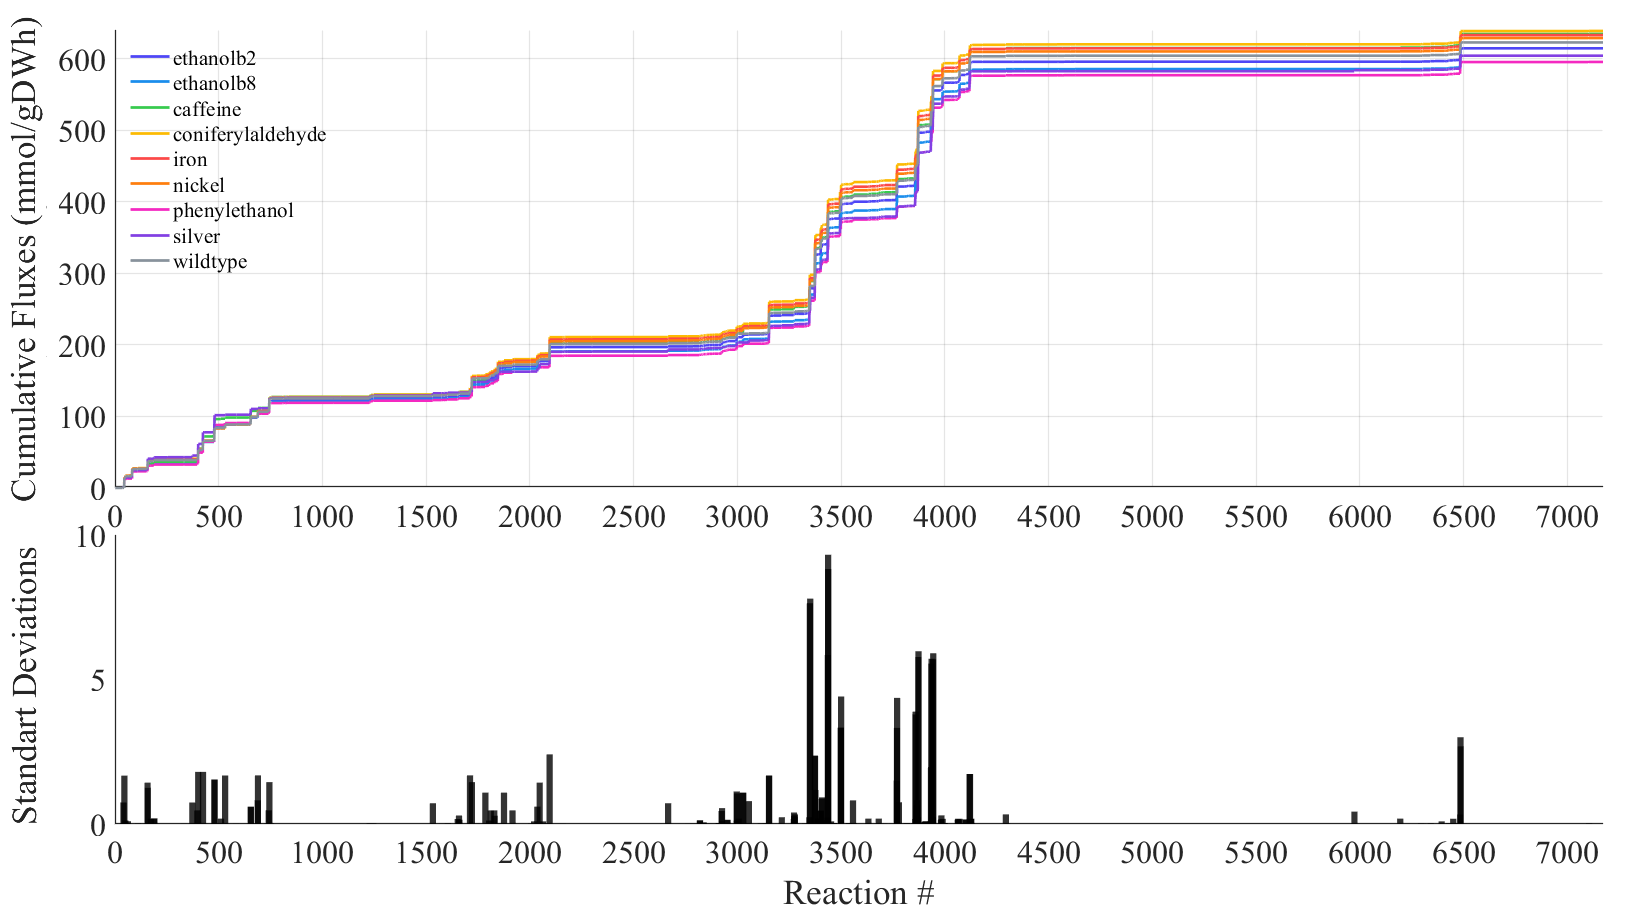
\includegraphics[width=1\columnwidth]{figures/cumflux_gur10.png}
  \caption[Cumulative flux vectors of each experiment when glucose uptake rate is constrained]{Cumulative flux vectors of each simulation and standart deviations. Glucose uptake rate is constrainted to 10 mmol/gDWh for all models. }
  \label{fig:cumflux_gur10}
  \end{center}
\end{figure}

Reactions with the standart deviation values more than 5 mmol/gDWh are listed in Table \ref{table:cumulative_free_stds}. Despite the decrease in the flux values (caused by the lower uptake rates of glucose), the top divergent reactions obtained are in agreement with the no-constraint flux balance analysis results.

\begin{table}[H]
\caption[The most divergent reactions across all strains and their flux values in mmol/gDWh when the glucose uptake rate is constrained to 10 mmol/gDWh.]{The most divergent reactions across all strains and their flux values in mmol/gDWh when the glucose uptake rate is constrained to 10 mmol/gDWh.}
\begin{center}
\setlength{\tabcolsep}{4pt}
\resizebox{\textwidth}{!}{
\begin{tabular}{|c|c|l|c|c|c|c|c|c|c|c|c|c|}
\hline
\textbf{\#} & \textbf{Gene} & \textbf{Reaction Name}                                                                     & \textbf{b2-eth} & \textbf{b8-eth} & \textbf{caff.} & \textbf{con. ald.} & \textbf{iron} & \textbf{nickel} & \textbf{phen.} & \textbf{silver} & \textbf{ref.} & \textbf{std} \\ \hline
1           & TDH1          & \begin{tabular}[c]{@{}l@{}}glyceraldehyde-\\ 3-phosphate \\ dehydrogenase (2)\end{tabular} & 17.64           & 0               & 0              & 17.48              & 0             & 17.54           & 0              & 18.18           & 17.55             & 9.32         \\ \hline
2           & TDH2          & \begin{tabular}[c]{@{}l@{}}glyceraldehyde-\\ 3-phosphate \\ dehydrogenase (3)\end{tabular} & 0               & 17.7            & 0              & 0                  & 17.51         & 0               & 17.71          & 0               & 0                 & 8.82         \\ \hline
4           & ERR3          & enolase (4)                                                                                & 0               & 17.43           & 0              & 0                  & 0             & 0               & 0              & 17.93           & 0                 & 7.8          \\ \hline
5           & ENO1          & enolase (2)                                                                                & 17.36           & 0               & 17.54          & 17.18              & 17.22         & 17.25           & 17.45          & 0               & 17.26             & 7.64         \\ \hline
6           & GPM1          & \begin{tabular}[c]{@{}l@{}}phosphoglycerate \\ mutase (2)\end{tabular}                     & 0               & 0               & 0              & 0                  & 0             & 0               & 0              & 17.93           & 0                 & 5.98         \\ \hline
8           & PYK2          & pyruvate kinase (2)                                                                        & 0               & 0               & 0              & 0                  & 0             & 0               & 0              & 17.72           & 0                 & 5.91         \\ \hline
9           & TDH3          & \begin{tabular}[c]{@{}l@{}}glyceraldehyde-\\ 3-phosphate \\ dehydrogenase (1)\end{tabular} & 0               & 0               & 17.54          & 0                  & 0             & 0               & 0              & 0               & 0                 & 5.85         \\ \hline
10          & YOR283W       & \begin{tabular}[c]{@{}l@{}}phosphoglycerate \\ mutase (1)\end{tabular}                     & 17.36           & 17.43           & 17.54          & 17.18              & 17.22         & 17.25           & 17.45          & 0               & 17.26             & 5.78         \\ \hline
11          & PDC5          & \begin{tabular}[c]{@{}l@{}}pyruvate \\ decarboxylase (3)\end{tabular}                      & 0               & 0               & 12.6           & 0                  & 9.08          & 0               & 12.15          & 0               & 0                 & 5.72         \\ \hline
12          & CDC19         & \begin{tabular}[c]{@{}l@{}}pyruvate \\ kinase (1)\end{tabular}                             & 17.12           & 17.21           & 17.31          & 16.93              & 16.97         & 17.01           & 17.23          & 0               & 17.01             & 5.7          \\ \hline
13          & PDC1          & \begin{tabular}[c]{@{}l@{}}pyruvate \\ decarboxylase (2)\end{tabular}                      & 10.36           & 11.08           & 0              & 8.69               & 0             & 9.37            & 0              & 14.54           & 9.42              & 5.55         \\ \hline
\end{tabular}}
\label{table:cumulative_gur10_stds}
\end{center}
\end{table}


Finally, only the arm reactions (where the isozyme reactions were seperated from, see Methods) when the glucose uptake rate is constrained to 10 mmol/gDWh are plotted as heatmap in Figure \ref{fig:fba_heatmap}. Arm reactions in this context refer to the combined reactions that normally have multiple sub-reactions because of isozymes catalyzing the same reaction. As it can be seen from the previous tables, most of the differences were caused by the isozymes with the flux values close to each other. By considering only arm reactions and a fixed glucose uptake rate, the reactions that actually differ because of the expression integration are found.

\begin{figure}[H]
  \begin{center}
  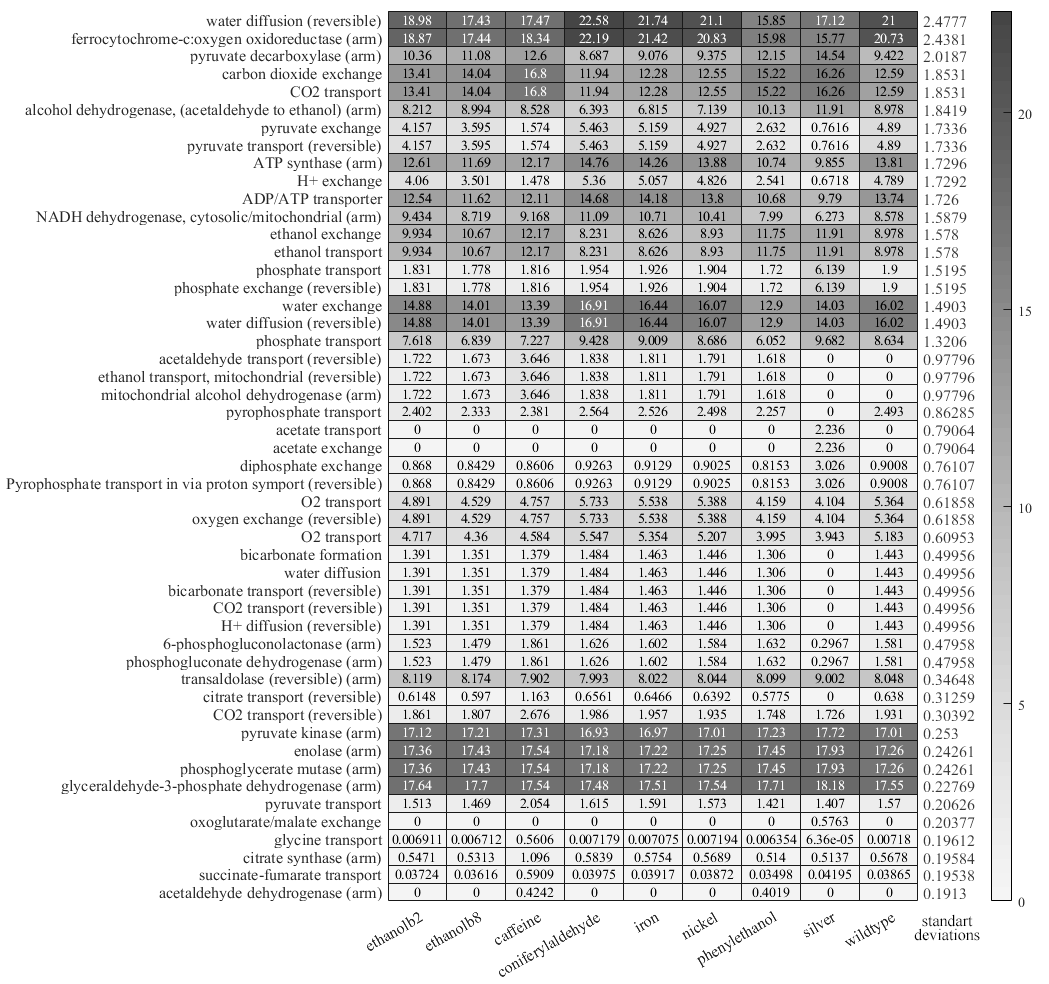
\includegraphics[width=1\columnwidth]{figures/fba_heatmap.png}
  \caption[Heatmap of the reaction fluxes where the standart deviation between models are the highest (top 50). Reversible means the intake of a substrate, arm means the flux of the reaction consists of isozyme reactions]{Heatmap of the reaction fluxes where the standart deviation between models are the highest (top 50). Reversible means the intake of a substrate, arm means the flux of the reaction consists of isozyme reactions.}
  \label{fig:fba_heatmap}
  \end{center}
\end{figure}

Overall the most divergent strain can be seen as silver resistant strain while the nickel strain has the closest values to the wildtype model as expected considering the integrated expression data. The highest deviation caused in the water diffusion from mitochondria to cytoplasm indicates that even at the same glucose feeding rates, phenylethanol resistant strain requires higher (89.5\%) water in the mitochondria. Followed with the ferrocytochrome-c:oxygen oxidoreductase, pyruvate decarboxylase reactions and different exchange reactions, the results conclude that the models of evolved strains follow different paths to produce biomass with the same environmental conditions provided.

As these different models belong to evolved strains, hierarchical relationship between models are drawn as dendrogram in Figure \ref{fig:fba_dendrogram}. Euclidean pairwise distance is calculated in MATLAB between flux balance analysis solution vectors for each model where the glucose uptake rate is constrained to 10 mmol/gDWh first and then clustered by the unweighted average distance (UPGMA) method to draw a tree. Cophenetic correlation coefficient is found as 0.9744 while theSpearman's rank correlation between the dissimilarities and the cophenetic distances is calculated as 0.9096, indicating a high-quality solution.

\begin{figure}[H]
  \begin{center}
  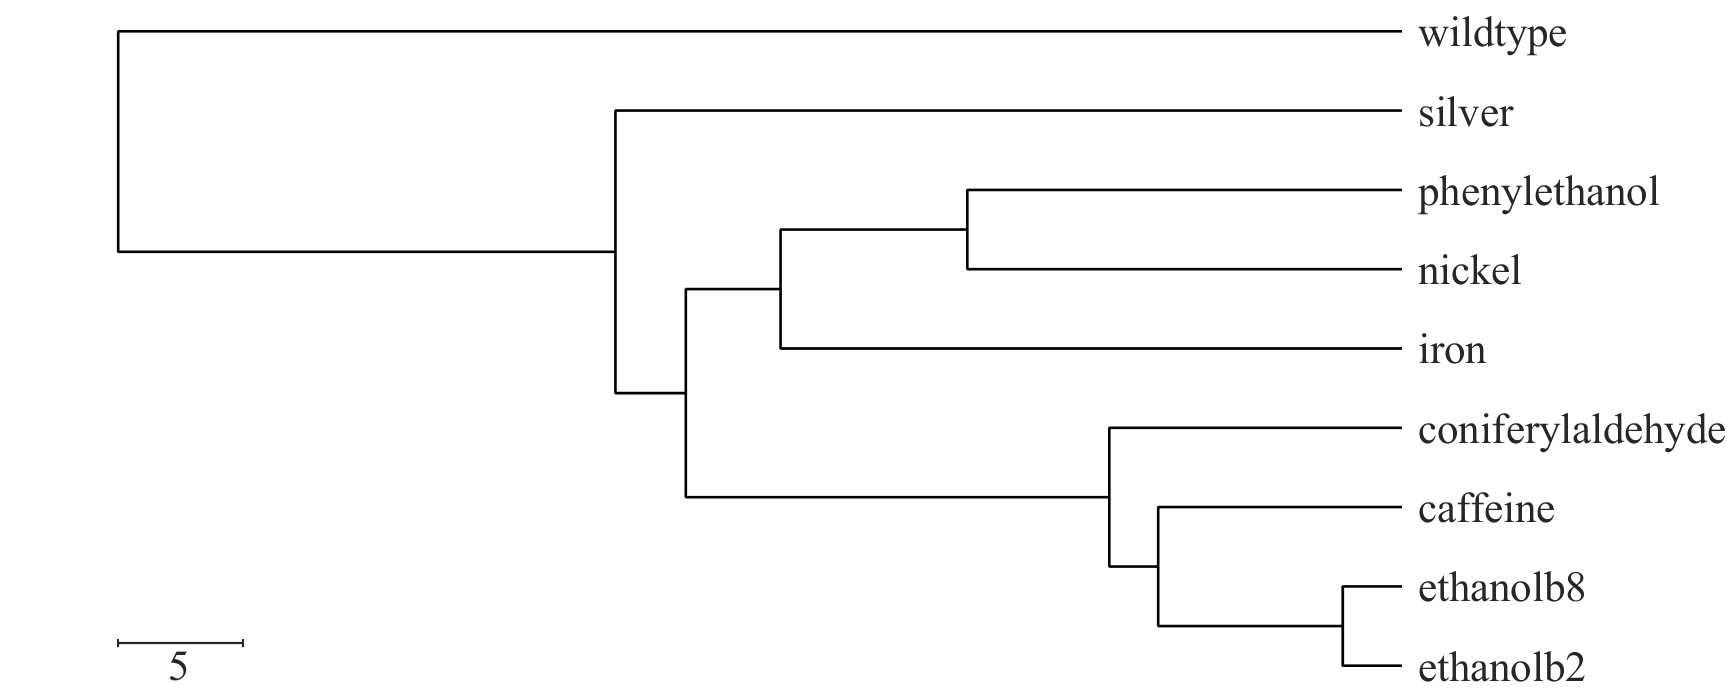
\includegraphics[width=1\columnwidth]{figures/fba_dendrogram.png}
  \caption[Hierarchical relationships between the strains drawn as a dendrogram plot. Euclidian distances are calcualted from the reaction fluxes (flux balance analysis) where the glucose uptake rate is constrained to 10 mmol/gDWh]{Hierarchical relationships between the strains drawn as a dendrogram plot. Euclidian distances are calcualted from the reaction fluxes (flux balance analysis) where the glucose uptake rate is constrained to 10 mmol/gDWh.}
  \label{fig:fba_dendrogram}
  \end{center}
\end{figure}

Despite the high correlation between the fold changes obtained from differential expression analysis and the flux balance analyses for particular enzymes, outliers must be investigated for the indirect regulation of enzymes. Three groups can be formed for these: Firstly, enzymes may show transcriptional regulation behaviors (TR) if their flux fold changes (between evolved and wildtype strain models) correlate with the differential gene expression results. Secondly, enzymes may show metabolic regulation behaviors (MR) if the flux change is observed even in the absences of the expressional changes. And lastly, enzymes may show post-transcriptional regulation behaviors (PR) if their expression levels change without showing any flux changes (Table \ref{table:regulation_table}). In the Figure \ref{fig:fba_regulation}, enzymes that have significant expressional fold changes (p $<$ 0.05) in all models are categorized for this purpose.

\vskip 1\baselineskip
\begin{table}[H]
\begin{center}
\caption[Enzymatic regulation decision table of expressional fold change (from differential analysis) and flux fold change (from flux balance analysis) comparison.]{Enzymatic regulation decision table of expressional fold change (from differential analysis) and flux fold change (from flux balance analysis) comparison.}
\vskip 0.5\baselineskip
\label{table:regulation_table}
\begin{tabular}{l|l|l|l|}
\cline{2-4}
\textbf{ExprFC \textbackslash FluxFC} & \textbf{Positive} & \textbf{Negative} & \textbf{No Change} \\ \hline
\multicolumn{1}{|l|}{\textbf{Positive}}  & Transcriptional & Metabolic       & Post-transcriptional \\ \hline
\multicolumn{1}{|l|}{\textbf{Negative}}  & Metabolic       & Transcriptional & Post-transcriptional \\ \hline
\multicolumn{1}{|l|}{\textbf{No Change}} & Metabolic       & Metabolic       &                      \\ \hline
\end{tabular}
\end{center}
\end{table}

Interestingly, most of the enzymes show post-transcriptional regulation behaviors indicating that even though the expression values are found significantly changed in the microarray analysis, their carried flux values did not differ in the \emph{in silico} simulations. Single simulation differences (such as FAS1, DFR1, CHO1 and ERG11 genes showing transcriptional regulation in all models except nickel model where they show metabolic regulation) must be investigated in order to understand the causal relationship.

\begin{figure}[H]
  \begin{center}
  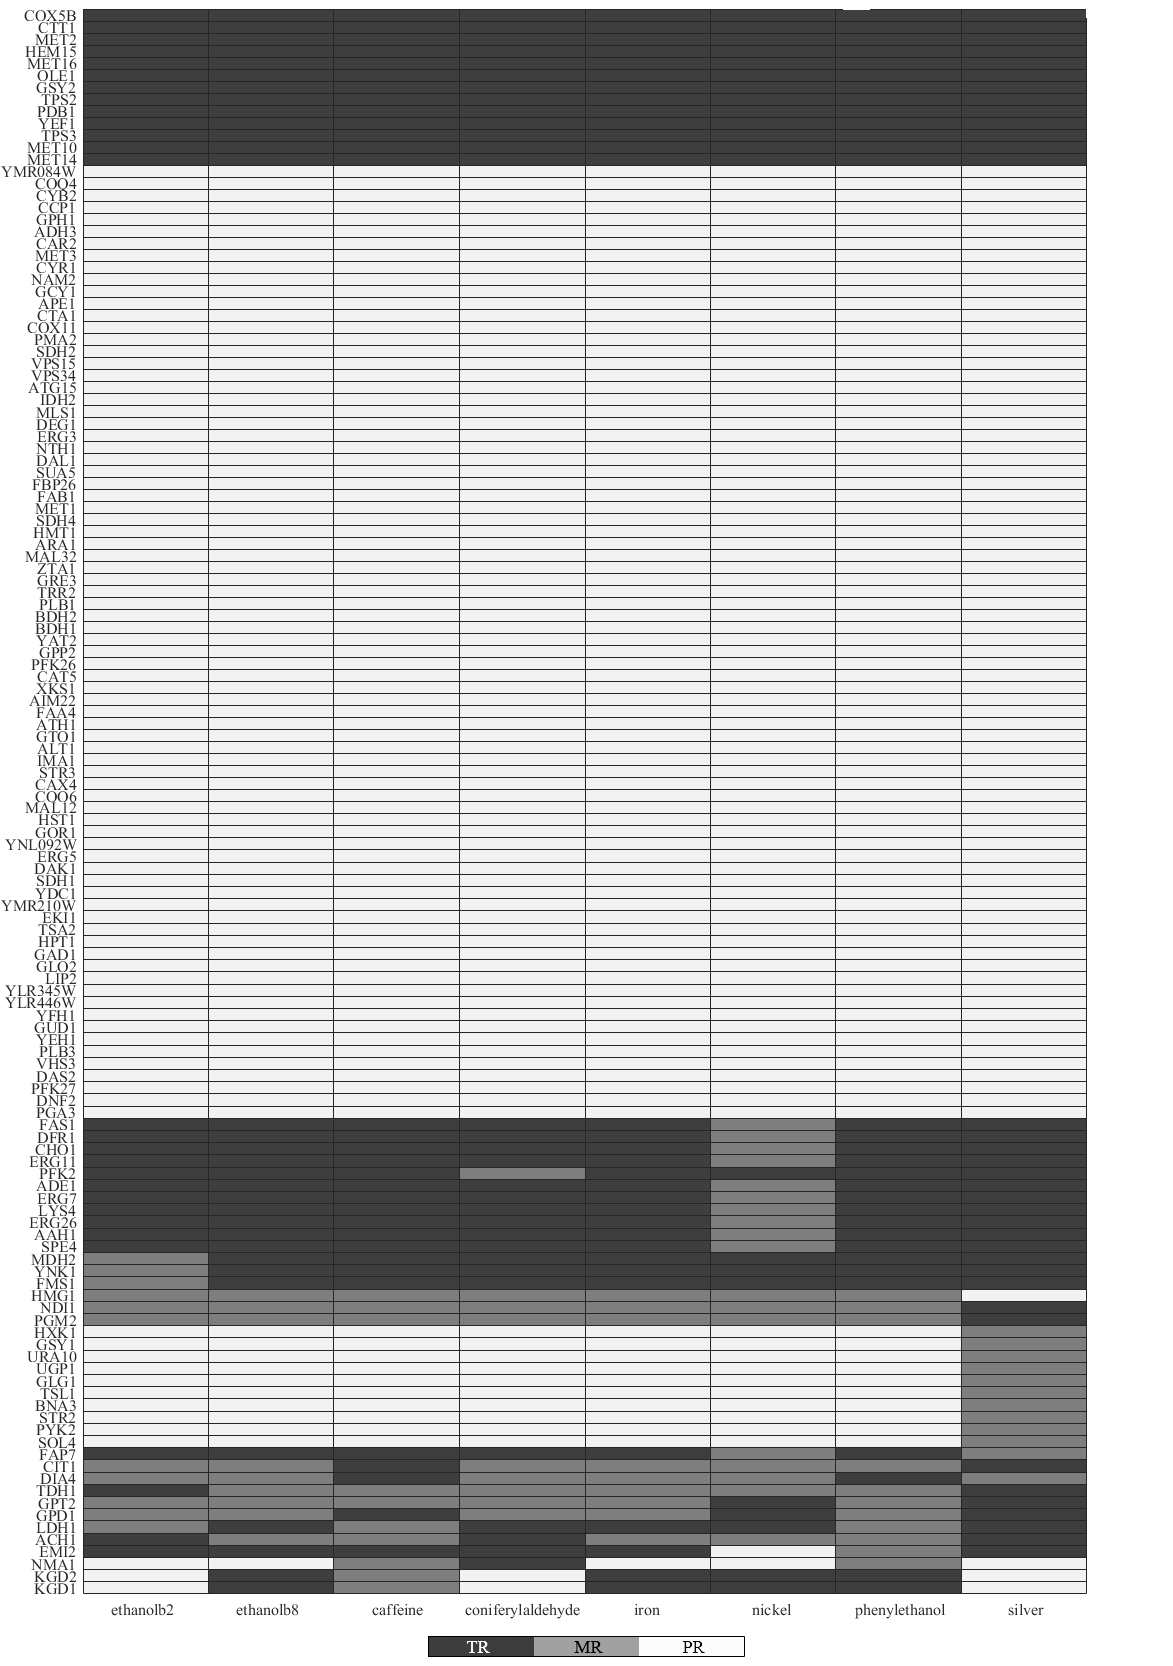
\includegraphics[width=1\columnwidth]{figures/fba_regulation2.png}
  \caption[Categorization of enzymes for regulation points for transcriptional regulation (TR), metabolic regulation (MR), post-transcriptional regulation (PR)]{Categorization of enzymes for regulation points for transcriptional regulation (TR), metabolic regulation (MR), post-transcriptional regulation (PR).}
  \label{fig:fba_regulation}
  \end{center}
\end{figure}

Shadow prices are calculated by solving the optimization problem for the objective function (growth rate) by increasing the upper constraints by one unit for all reactions. This way, the sensitivity of the reactions to the growth rate is calculated for all models. In Table \ref{table:fba_shadowprices_free_table}, the shadow prices of the reactions that limit the growth rate more than itself and their values can be seen. The values for each reaction are divided to the wild-type model's shadow price values to uncover the adaptive evolution effects and plotted in Figure \ref{fig:fba_shadowprices_free}.

\vskip 1\baselineskip
\begin{table}[H]
\caption[Shadow prices of the exchange metabolites' uptake reactions that has a value higher than the growth itself]{Shadow prices of the exchange metabolites' uptake reactions that has a value higher than the growth itself.}
\vspace{-0.3cm}
\begin{center}
\setlength{\tabcolsep}{4pt}
\resizebox{\textwidth}{!}{
\begin{tabular}{|l|c|c|c|c|c|c|c|c|c|}
\hline
\textbf{\begin{tabular}[c]{@{}l@{}}exchange \\ metabolites\end{tabular}} &   \textbf{b2-eth} &   \textbf{b8-eth} &   \textbf{caff.} &   \textbf{con. ald.} &   \textbf{iron} &   \textbf{nickel} &   \textbf{phen.} &   \textbf{silver} &   \textbf{ref.} \\ \hline
biotin                                                                            & -78.78 & -76.60 & -38.46 & -104.17 & -82.63 & -99.87 & -32.60 & -255.57 & -100.10 \\ \hline
riboflavin                                                                        & -44.24 & -44.65 & -43.65 & -47.91  & -36.10 & -46.06 & -27.84 & -65.51  & -46.16  \\ \hline
\begin{tabular}[c]{@{}l@{}}flavin mono- \\ nucleotide (FMN)\end{tabular}                                                                                & -44.24 & -44.65 & -43.65 & -47.91  & -36.10 & -46.06 & -27.84 & -65.51  & -46.16  \\ \hline
\begin{tabular}[c]{@{}l@{}}5-formyltetrahydro- \\ folic acid\end{tabular}           & -13.92 & -12.99 & -16.91 & -14.40  & -13.70 & -14.69 & -11.86 & -16.92  & -14.72  \\ \hline
4-aminobenzoate                                                                   & -6.81  & -6.68  & -7.41  & -7.50   & -7.21  & -7.19  & -5.09  & -8.69   & -7.20   \\ \hline
ergosterol                                                                        & -3.47  & -2.93  & -2.41  & -3.30   & -2.85  & -3.75  & -2.42  & -5.77   & -3.76   \\ \hline
\begin{tabular}[c]{@{}l@{}}ergosta-5,7,22,24-\\ (28)-tetraen-3beta-ol\end{tabular} & -3.38  & -2.86  & -2.35  & -3.21   & -2.76  & -3.67  & -2.37  & -5.65   & -3.67   \\ \hline
zymosterol                                                                        & -3.19  & -2.67  & -2.21  & -3.04   & -2.59  & -3.46  & -2.24  & -5.28   & -3.46   \\ \hline
14-demethyllanosterol                                                             & -2.95  & -2.47  & -2.02  & -2.79   & -2.32  & -3.14  & -1.99  & -4.94   & -3.14   \\ \hline
hexanoate                                                                         & -2.69  & -3.43  & -6.28  & -5.48   & -4.91  & -3.56  & -5.11  & -2.07   & -3.58   \\ \hline
lanosterol                                                                        & -2.13  & -1.84  & -1.60  & -1.88   & -1.67  & -2.26  & -1.57  & -3.31   & -2.26   \\ \hline
growth                                                                            & -1     & -1     & -1     & -1      & -1     & -1     & -1     & -1      & -1      \\ \hline
\end{tabular}}
\label{table:fba_shadowprices_free_table}
\end{center}
\end{table}


\begin{figure}[H]
  \begin{center}
  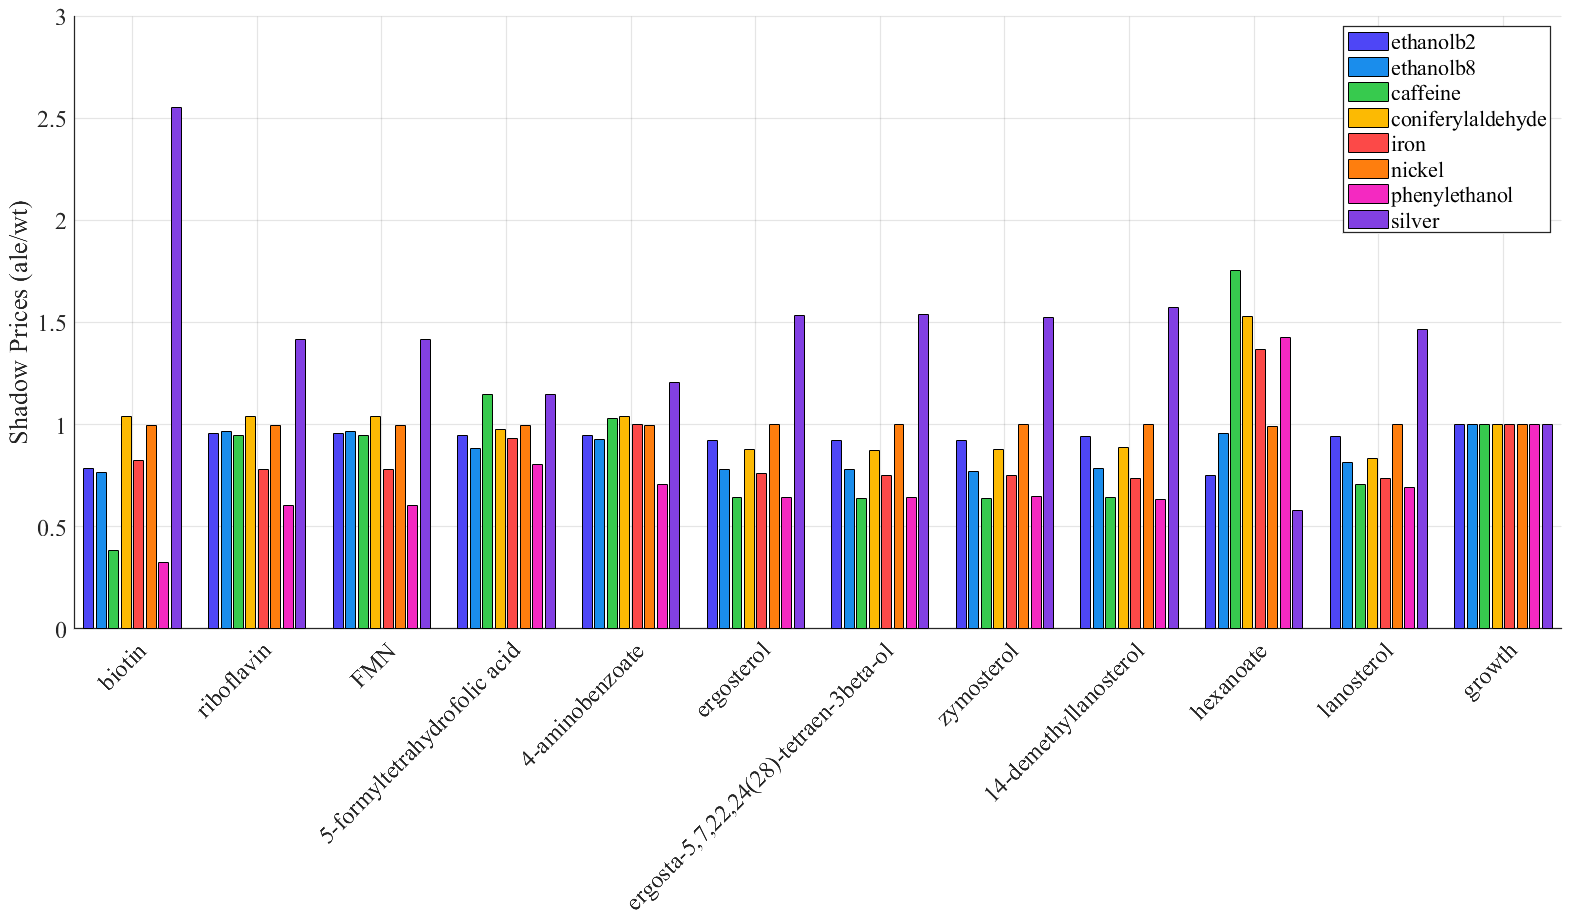
\includegraphics[width=1\columnwidth]{figures/fba_shadowprices_free.png}
  \caption[Barplots of the changes in the shadow prices of the metabolites that have contibutions higher than the biomass (growth) itself. Shadow price of each reaction for evolved models is divided by the shadow price of that reaction in the wildtype model]{Barplots of the changes in the shadow prices of the metabolites that have contibutions higher than the biomass (growth) itself. Shadow price of each reaction for evolved models is divided by the shadow price of that reaction in the wildtype model.}
  \label{fig:fba_shadowprices_free}
  \end{center}
\end{figure}

Shadow prices of metabolites show us that the metabolites zymosterol, ergosta-5,7,22,24(28)-tetraen-3beta-ol, ergosterol, lanosterol, 14-demethyllanosterol, biotin, riboflavin, flavin mononucleotide (FMN), 5-formyltetrahydrofolic acid, 4-aminobenzoate and hexanoate are the most required metabolites in the media to increase growth rate in all models, in order for their mean values across models. Although all the models would increase their biomass production with these metabolites supplied, increment amounts would differ for each model. While the silver resistant model would increase its growth rate by 250\% with biotin supplement, phenylethanol resistant model could only achieve 33\% increase.

When we look at the main ATP producing reactions in the metabolic models, wee see the pyruvate kinase reactions (Eq. \ref{eq:PK}),
\begin{align}
\label{eq:PK}
\ ADP + H^+ + phosphoenolpyruvate \xrightarrow{PK} ATP + pyruvate
\end{align}
and phosphoglycerate kinase reactions (Eq. \ref{eq:PGK1}),
\begin{align}
\begin{split}
\label{eq:PGK1}
\ 1,3-bisphospho-D-glycerate + ADP  \xrightarrow{PGK1} \\
\ 3-phosphonato-D-glycerate^{3-} + ATP
\end{split}
\end{align}
are actively used. Comparison between fluxes through these ATP producing reactions under both free system (where the only constraint is the availability of protein levels) and constrained system (where additional constraint to glucose uptake rate is applied, 10 mmol/gDWh) can be found in Table \ref{table:fba_atp_production}.

\vskip 1\baselineskip
\begin{table}[H]
\centering
\caption[Carried flux values (mmol/gDWh) through ATP producing reactions (A: the only constraint applied to the models is the maximum protein availability; B: additional constraint is applied to the glucose uptake rate as 10 mmol/gDW)]{Carried flux values (mmol/gDWh) through ATP producing reactions (A: the only constraint applied to the models is the maximum protein availability; B: additional constraint is applied to the glucose uptake rate as 10 mmol/gDW).}
\vspace{0.2cm}
\label{table:fba_atp_production}
\setlength{\tabcolsep}{4pt}
\resizebox{\textwidth}{!}{
\begin{tabular}{l|c|c|c|c|c|c|c|c|c|c|c|c|c|c|c|c|c|c|}
\cline{2-19}
 &
  \multicolumn{2}{c|}{\textbf{ethanolb2}} &
  \multicolumn{2}{c|}{\textbf{ethanolb8}} &
  \multicolumn{2}{c|}{\textbf{caffeine}} &
  \multicolumn{2}{c|}{\textbf{\begin{tabular}[c]{@{}c@{}}coniferyl\\ aldehyde\end{tabular}}} &
  \multicolumn{2}{c|}{\textbf{iron}} &
  \multicolumn{2}{c|}{\textbf{nickel}} &
  \multicolumn{2}{c|}{\textbf{\begin{tabular}[c]{@{}c@{}}phenyl\\ ethanol\end{tabular}}} &
  \multicolumn{2}{c|}{\textbf{silver}} &
  \multicolumn{2}{c|}{\textbf{wildtype}} \\ \cline{2-19}
 &
  \textbf{A} &
  \textbf{B} &
  \textbf{A} &
  \textbf{B} &
  \textbf{A} &
  \textbf{B} &
  \textbf{A} &
  \textbf{B} &
  \textbf{A} &
  \textbf{B} &
  \textbf{A} &
  \textbf{B} &
  \textbf{A} &
  \textbf{B} &
  \textbf{A} &
  \textbf{B} &
  \textbf{A} &
  \textbf{B} \\ \hline
\multicolumn{1}{|l|}{Pyruvate kinase} &
  23.6 &
  17.1 &
  27.8 &
  17.2 &
  48.5 &
  17.3 &
  36.2 &
  16.9 &
  24.8 &
  17.0 &
  32.2 &
  17.0 &
  32.2 &
  17.2 &
  36.9 &
  17.7 &
  32.3 &
  17.0 \\ \hline
\multicolumn{1}{|l|}{\begin{tabular}[l]{@{}c@{}}Phosphoglycerate\\ kinase\end{tabular}} &
  24.1 &
  17.6 &
  28.3 &
  17.7 &
  48.8 &
  17.5 &
  36.8 &
  17.5 &
  25.3 &
  17.5 &
  32.8 &
  17.5 &
  32.7 &
  17.7 &
  37.4 &
  18.2 &
  32.9 &
  17.6 \\ \hline
\multicolumn{1}{|l|}{ATP Synthase} &
  7.0	&
  12.5	&
  4.2	&
  11.6	&
  0	&
  12.1	&
  0.1	&
  14.7	&
  7.7	&
  14.2	&
  0.1	&
  13.8	&
  0	&
  10.7	&
  0.0	&
  9.8	&
  0.1	&
  13.7  \\ \hline
\multicolumn{1}{|l|}{\textbf{Total}} &
54.8	&
47.3	&
60.3	&
46.5	&
97.2	&
47.0	&
73.2	&
49.1	&
57.8	&
48.7	&
65.2	&
48.4	&
65.0	&
45.6	&
74.3	&
45.7	&
65.3	&
48.3 \\ \hline
\end{tabular}}
\end{table}


Total values of ATP production do not differ when the carbon supply is almost the same for all models. On the other hand, if we compare the simulation under free carbon source (NC columns), differences arise. We should consider maximum growth rate and glucose uptake rate for these models, therefore Figure \ref{fig:fba_gro_glu_atp} is created with the values from Table \ref{table:growth_glucose_table}.

\begin{figure}[H]
  \begin{center}
  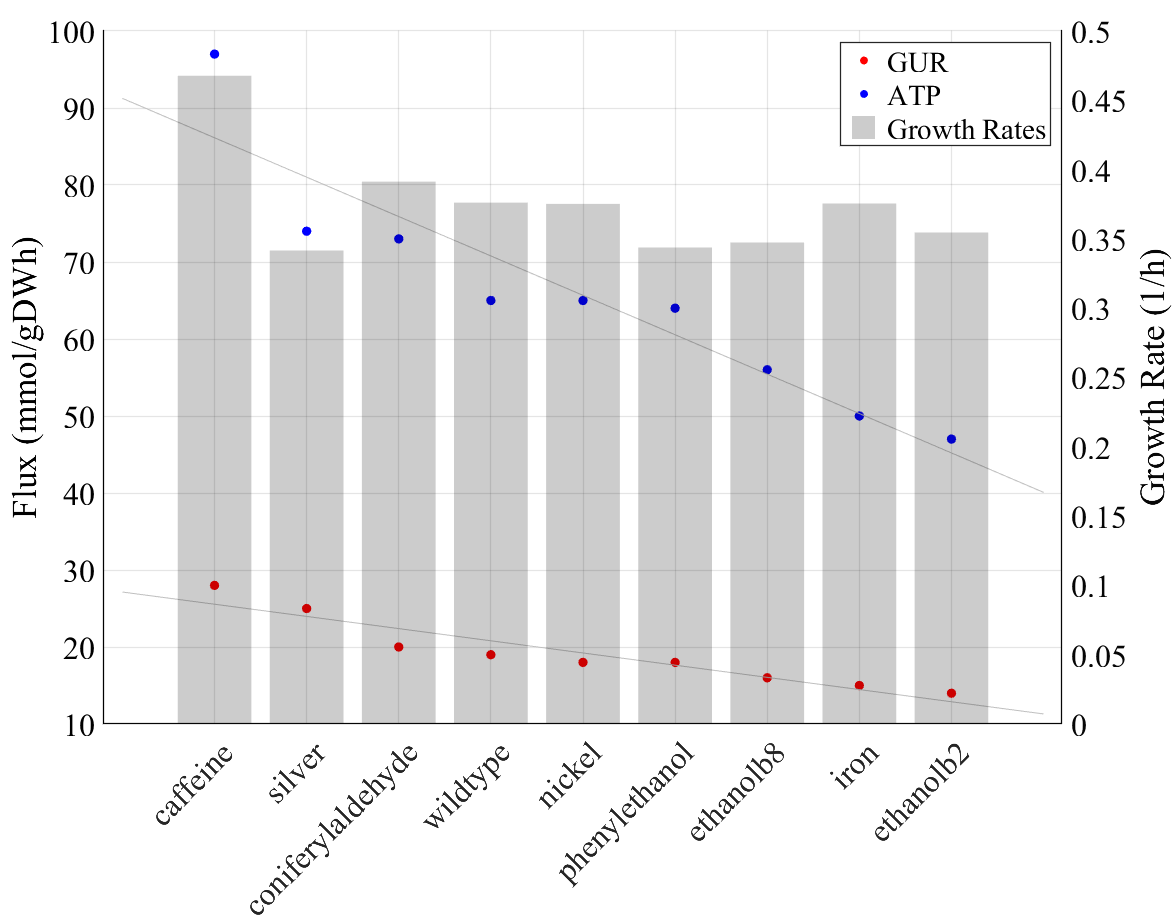
\includegraphics[width=1\columnwidth]{figures/fba_gro_glu_atp.png}
  \caption[Glucose uptake rates and total fluxes through ATP producing reactions are plotted with least-squares lines. Growth rates are shown as bar graphs.]{Glucose uptake rates and total fluxes through ATP producing reactions are plotted with least-squares lines. Growth rates are shown as bars on the secondary y-axis.}
  \label{fig:fba_gro_glu_atp}
  \end{center}
\end{figure}

As expected for the caffeine resistant model which has the highest glucose uptake rate and the total ATP production flux, it has the highest growth rate among all models. Silver resistant model however, has a lower growth rate considering having the second highest glucose uptake rate and total ATP production flux. Despite the lower fluxes on the glucose uptake and atp production, the iron resistant model shows higher growth rates. The similar values from wiltype and nickel resistant models were also expected since the lowest amount of gene expression information was integrated for the nickel resistant model, making it the least differentiated model from the wildtype.

\begin{figure}[H]
  \begin{center}
  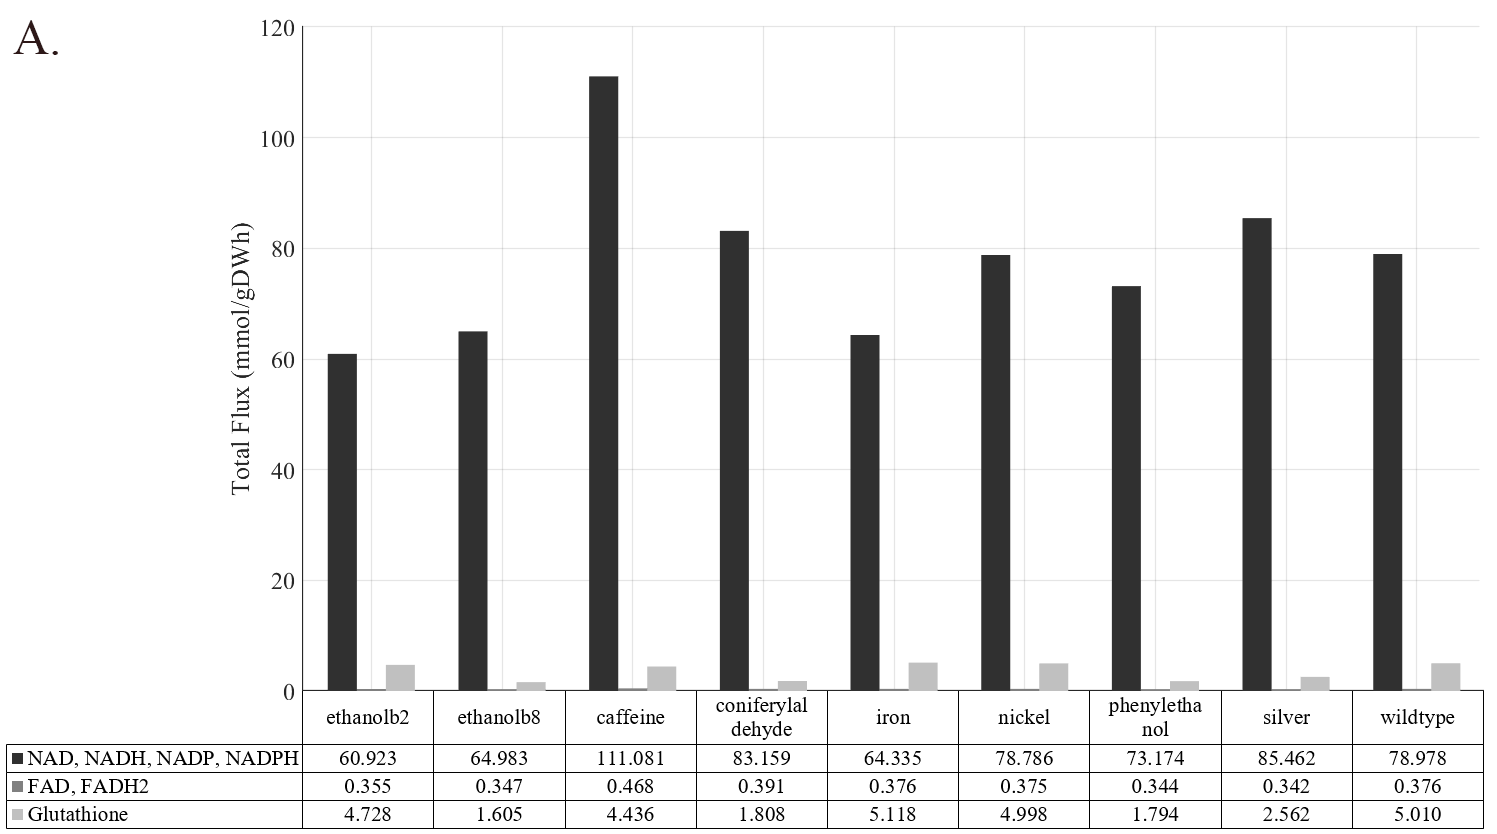
\includegraphics[width=1\columnwidth]{figures/fba_nad_fad_free_bw.png}
  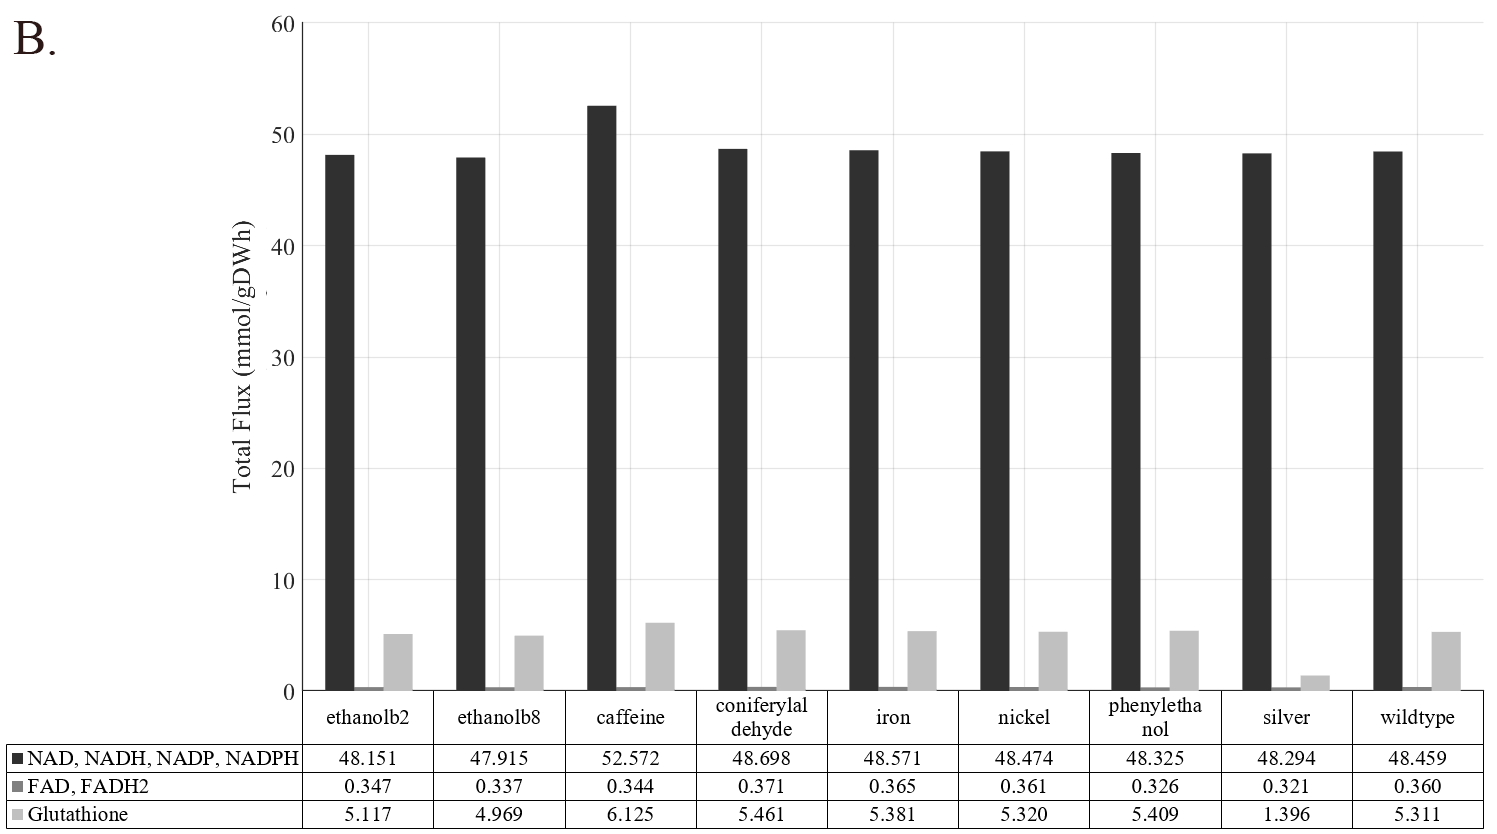
\includegraphics[width=1\columnwidth]{figures/fba_nad_fad_gur10_bw.png}
  \caption[Total flux values of NAD/NADP, FAD consumption and glutathione metabolism reactions of the simulations where  no additional constraint to uptake reactions is applied (TOP), and the glucose uptake rate is constained to 10 mmol/gDWh (BOTTOM), for each model]{Total flux values of NAD/NADP, FAD consumption and glutathione metabolism reactions of the simulations where  no additional constraint to uptake reactions is applied (TOP), and the glucose uptake rate is constained to 10 mmol/gDWh (BOTTOM), for each model.}
  \label{fig:fba_nad_fad}
  \end{center}
\end{figure}

When we look at the total coenzymes NAD, NADP, FAD consumptions and the glutathione metabolism fluxes, similar results to the ATP regulations are observed with the exception of a significant difference on the glutathione metabolism in the silver resistant model. When the glucose uptake rate is constrained same for all models, we have collected similar results from all models. Surprisingly, the silver resistant model was not able to carry high fluxes through glutathione metabolism under the same glucose uptake rate conditions. This could explain why the silver resistant model was unable to grow at high rates depite carrying high fluxes on the glucose uptake and ATP producing reactions (Figure \ref{fig:fba_gro_glu_atp}).


Flux distribution within the amino acid biosynthesis subsystem in the models are collected in the Table \ref{table:aminoacids_free}. The reactions enolase, phosphoglycerate mutase, pyruvate kinase, glyceraldehyde-3-phosphate dehydrogenase are the most active reactions in the amino acid biosynthesis. Although the most of the flux values are in parallel with the corresponding glucose uptake rates, some differences are observed. 2-isopropylmalate synthase enzyme is only used by coniferylaldehyde andiron resistant models. While caffeine resistant model chooses to use 3-deoxy-D-arabino-heptulosonate 7-phosphate synthetase enzyme, all other models carry their fluxes through 2-deoxy-D-arabino-heptulosonate 7-phosphate synthetase. The caffeine resistant model also does not carry a flux through phosphoglycerate dehydrogenase. And most interestingly, the silver resistant model carries flux in the reverse direction through transketolase 1 and transketolase 2 reactions (Eq. \ref{eq:transketolase} shows the forward directions) with lower values.
\begin{align}
\begin{split}
\label{eq:transketolase}
\ D-xylulose-5-phosphate + ribose-5-phosphate \xrightarrow{transketolase1} \\
\ glyceraldehyde-3-phosphate + sedoheptulose-7-phosphate \\
\ \\
\ D-erythrose-4-phosphate + D-xylulose-5-phosphate \xrightarrow{transketolase2} \\
\ D-fructose-6-phosphate + glyceraldehyde-3-phosphate
\end{split}
\end{align}

\vskip 1\baselineskip
\begin{table}[H]
  \small
  \centering
  \caption[Fluxes through the reactions in the amino acids biosynthesis subsystem]{Fluxes through the reactions in the amino acids biosynthesis subsystem.}
  \label{table:aminoacids_free}
  \setlength{\tabcolsep}{4pt}
  \resizebox{\textwidth}{!}{

  \begin{tabular}{|l|c|c|c|c|c|c|c|c|c|}
  \hline
  \textbf{Reactions}                                                                                   & \textbf{b2-eth.} & \textbf{b8-eth.} & \textbf{caff.} & \textbf{con. ald.} & \textbf{iron} & \textbf{nickel} & \textbf{phen.} & \textbf{silver} & \textbf{ref.} \\ \hline
  \begin{tabular}[c]{@{}l@{}}2-aceto-2-hydroxy-\\ butanoate synthase\end{tabular}                      & 0.085              & 0.084              & 0.113             & 0.094                                                                  & 0.090         & 0.090           & 0.083                  & 0.082           & 0.091             \\
  \begin{tabular}[c]{@{}l@{}}2-aminoadipate \\ transaminase\end{tabular}                               & 0.127              & 0.124              & 0.167             & 0.140                                                                  & 0.134         & 0.134           & 0.123                  & 0.122           & 0.134             \\
  \begin{tabular}[c]{@{}l@{}}2-deoxy-D-arabino-\\ heptulosonate-7-\\ phosphate synthetase\end{tabular} & 0.119              & 0.117              & 0                 & 0.132                                                                  & 0.126         & 0.126           & 0.116                  & 0.115           & 0.126             \\
2-isopropylmalate synthase                                & 0                  & 0                  & 0                 & 0.145                                                                  & 0.139         & 0               & 0                      & 0               & 0                 \\
  \begin{tabular}[c]{@{}l@{}}3-deoxy-D-arabino-\\ heptulosonate-7-\\ phosphate synthetase\end{tabular} & 0                  & 0                  & 0.157             & 0                                                                      & 0             & 0               & 0                      & 0               & 0                 \\
  acetolactate synthase                                                                                & 0.249              & 0.243              & 0.328             & 0.274                                                                  & 0.263         & 0.263           & 0.241                  & 0.239           & 0.264             \\
  citrate synthase                                                                                     & 0.559              & 0.547              & 0.595             & 0.617                                                                  & 0.592         & 0.591           & 0.437                  & 0.539           & 0.593             \\
  enolase                                                                                              & 23.842             & 28.028             & 48.769            & 36.501                                                                 & 25.038        & 32.485          & 32.463                 & 37.133          & 32.564            \\
  \begin{tabular}[c]{@{}l@{}}glyceraldehyde-\\ 3-phosphate\\  dehydrogenase\end{tabular}               & 24.128             & 28.308             & 48.769            & 36.816                                                                 & 25.341        & 32.787          & 32.740                 & 37.397          & 32.867            \\
  homoacontinate hydratase                         & 0.127              & 0.124              & 0.167             & 0.140                                                                  & 0.134         & 0.134           & 0.123                  & 0.122           & 0.134             \\
  \begin{tabular}[c]{@{}l@{}}methionine \\ adenosyltransferase\end{tabular}                            & 0.046              & 0.045              & 0.061             & 0.051                                                                  & 0.049         & 0.049           & 0.045                  & 0.045           & 0.049             \\
  \begin{tabular}[c]{@{}l@{}}O-succinylhomoserine \\ lyase (reverse)\end{tabular}                      & 0.003              & 0.003              & 0.004             & 0.003                                                                  & 0.003         & 0.003           & 0.003                  & 0.003           & 0.003             \\
  phosphofructokinase                                                                                  & 11.896             & 14.158             & 25.467            & 18.412                                                                 & 12.486        & 16.216          & 16.356                 & 20.641          & 16.256            \\
  \begin{tabular}[c]{@{}l@{}}phosphoglycerate \\ dehydrogenase\end{tabular}                            & 0.286              & 0.280              & 0                 & 0.315                                                                  & 0.302         & 0.302           & 0.277                  & 0.264           & 0.303             \\
  \begin{tabular}[c]{@{}l@{}}phosphoglycerate \\ mutase\end{tabular}                                   & 23.842             & 28.028             & 48.769            & 36.501                                                                 & 25.038        & 32.485          & 32.463                 & 37.133          & 32.564            \\
  \begin{tabular}[c]{@{}l@{}}phosphoribosylpyro-\\ phosphate synthetase\end{tabular}                   & 0.121              & 0.118              & 0.159             & 0.133                                                                  & 0.128         & 0.128           & 0.117                  & 0.116           & 0.128             \\
  pyruvate carboxylase                                                                                 & 1.264              & 1.237              & 2.450             & 1.394                                                                  & 1.121         & 1.337           & 0.899                  & 0.902           & 1.340             \\
  pyruvate kinase                                                                                      & 23.603             & 27.795             & 48.454            & 36.238                                                                 & 24.786        & 32.233          & 32.232                 & 36.903          & 32.311            \\
  transaldolase (rev.)                                                                              & 11.434             & 14.041             & 25.041            & 18.281                                                                 & 11.984        & 15.728          & 16.206                 & 20.642          & 15.766            \\
  transketolase 1                                                                                      & 0.462              & 0.117              & 0.426             & 0.132                                                                  & 0.502         & 0.489           & 0.150                  & 0               & 0.490             \\
  transketolase 1 (rev.)                                                                            & 0                  & 0                  & 0                 & 0                                                                      & 0             & 0               & 0                      & 0.001           & 0                 \\
  transketolase 2                                                                                      & 0.343              & 0                  & 0.268             & 0                                                                      & 0.376         & 0.363           & 0.034                  & 0               & 0.364             \\
  transketolase 2 (rev.)                                                                            & 0                  & 0                  & 0                 & 0                                                                      & 0             & 0               & 0                      & 0.116           & 0                 \\ \hline
  \end{tabular}}
\end{table}


In the metabolic model, there are 12 branchpoint metabolites that considered the precursor metabolites for the central carbon metabolism in the network. Producing and consuming reactions of these 12 precursor metabolites (Table \ref{table:12precursors}) are investigated individually for all models.

\begin{table}[H]
\caption[The 12 precursor (branchpoint) metabolites for biomass production]{The 12 precursor (branchpoint) metabolites for biomass production.}
\setlength{\tabcolsep}{4pt}
\resizebox{\textwidth}{!}{\begin{tabular}{|c|l|c|l|}
\hline
\textbf{\#} & \textbf{Metabolite}           & \textbf{Abbreviation} & \textbf{Building Blocks Produced}         \\ \hline
1               & D-glucose-6-phosphate         & G6P                   & glycogen, LPS                             \\ \hline
2               & D-fructose-6-phosphate        & F6P                   & cell wall                                 \\ \hline
3               & D-ribose-5-phosphate          & R5P                   & His, Phe, Trp, nucleotides                \\ \hline
4               & D-erythrose-4-phosphate       & E4P                   & Phe, Trp, Tyr                             \\ \hline
5               & D-glyceraldehyde-3- phosphate & GAP                   & lipids                                    \\ \hline
6               & glycerate-3-phosphate         & 3PG                   & Cys, Gly, Ser                             \\ \hline
7               & phosphoenolpyruvate           & PEP                   & Tyr, Trp                                  \\ \hline
8               & pyruvate                      & PYR                   & Ala, Ile, Lys, Leu, Va                    \\ \hline
9               & acetyl-CoA                    & ACA                   & Leu, lipids                               \\ \hline
10              & 2-ketoglutarate               & 2KG                   & Glu, Gln, Arg, Pro                        \\ \hline
11              & succinyl-CoA                  & SCA                   & Met, Lys, tetrapyrroles (e.g., heme)      \\ \hline
12              & oxaloacetate                  & OXA                   & Asn, Asp, Ile, Lys, Met, Thr, nucleotides \\ \hline
\end{tabular}}
\label{table:12precursors}
\end{table}

For the start, hexokinase reaction is the only producing reaction for the first precursor metabolite D-glucose-6-phosphate (Eq. \ref{eq:12hexokinase}),
\begin{align}
\label{eq:12hexokinase}
\ ATP + \text{D-glucose} \xrightarrow{hexokinase} ADP + \text{D-glucose 6-phosphate} + \text{H+}
\end{align}
and the flux values for all models is the same as the provided glucose upate rate (in this case, 10 mmol/gDWh). The main difference is the active gene for the enzymes. While the silver resistant model prefers to use the nenzyme HXK1 (YFR053C), phenylethanol resistant model uses the enzyme HXK2 (YGL253W), while all the other models use EMI2 (YDR516C).

Consuming reactions for the for the G6P are the glucose-6-phosphate isomerase, glucose 6-phosphate dehydrogenase, phosphoglucomutase, alpha,alpha-trehalose-phosphate synthase (UDP-forming), and myo-inositol-1-phosphate synthase reaction. Sum of all the consuming reactions are the same as the production rate, 10 mmol/gDWh, as expected. The only emerging result is observed for the silver resistant model, where all models are carries flux through the isomerase reaction by 78.5\% and through dehydrogenase reaction by 16.2\% of total G6P consumption fluxes, the silver model carries 92.2\% through the isomerase reaction and 2.9\% for the dehydrogenase reaction.

Producing and consuming reaction fluxes for the metabolite D-fructose-6-phosphate (F6P) can be seen in the Table \ref{table:12F6P}. Similar to the G6P results, the only difference noticable arises from the silver resistant model.

\begin{table}[H]
\vspace{0.5cm}
\caption[Producing and consuming reaction fluxes for the metabolite D-fructose-6-phosphate (F6P).]{Producing and consuming reaction fluxes for the metabolite D-fructose-6-phosphate (F6P).}
\setlength{\tabcolsep}{4pt}
\resizebox{\textwidth}{!}{
\begin{tabular}{cllccccccccc}
\hline
\multicolumn{1}{l}{F6P} & Reaction Name                      & Genes                                                       & ethanolb2 & ethanolb8 & caffeine & \begin{tabular}[c]{@{}c@{}}coniferyl-\\ aldehyde\end{tabular} & iron & nickel & \begin{tabular}[c]{@{}c@{}}phenyl-\\ ethanol\end{tabular} & silver & wildtype \\ \hline
\multirow{2}{*}{\rotatebox[origin=c]{90}{Prod.}}    & glucose-6-phosphate isomerase & YBR196C                                                     & 7.95      & 8.01      & 7.62     & 7.82                                                          & 7.85 & 7.87   & 7.88                                                      & 9.22   & 7.88     \\
                        & transketolase 2               & YPR074C                                                     & 0.39      & 0.38      & 0.50     & 0.42                                                          & 0.41 & 0.41   & 0.43                                                      & 0      & 0.41     \\ \hline
\multirow{3}{*}{\rotatebox[origin=c]{90}{Consuming}}    & transaldolase                 & \begin{tabular}[c]{@{}l@{}}YLR354C, \\ YGR043C\end{tabular} & 8.12      & 8.17      & 7.90     & 7.99                                                          & 8.02 & 8.04   & 8.10                                                      & 9.00   & 8.05     \\
                        & mannose-6-phosphate isomerase & YER003C                                                     & 0.23      & 0.22      & 0.22     & 0.24                                                          & 0.24 & 0.23   & 0.21                                                      & 0.21   & 0.23     \\
                        & transketolase 2               & \begin{tabular}[c]{@{}l@{}}YBR117C,\\ YPR074C\end{tabular}  & 0         & 0         & 0        & 0                                                             & 0    & 0      & 0                                                         & 0.01   & 0        \\ \hline
\end{tabular}}
\label{table:12F6P}
\end{table}

The only reaction produces the metabolite d-ribulose-5-phosphate (R5P) in the network is the phosphogluconate dehydrogenase that has two isozymes GND1 (YHR183W) and GND2 (YGR256W). From the evolved model simulations, caffeine, coniferylaldehyde, iron, nickel and phenylethanol resistant models use the GND1 isozyme while ethanolb2, ethanolb8 and silver resistant models use the GND2 isozyme.

Ribulose 5-phosphate 3-epimerase and ribose-5-phosphate isomerase reactions are the only active reactions for the consumption of the R5P. Flux values of both production and consumption rates can be found in the Table \ref{table:12R5P}.

\begin{table}[H]
\vspace{0.5cm}
\caption[Producing and consuming reaction fluxes for the metabolite d-ribulose-5-phosphate (R5P).]{Producing and consuming reaction fluxes for the metabolite d-ribulose-5-phosphate (R5P).}
\setlength{\tabcolsep}{4pt}
\resizebox{\textwidth}{!}{
\begin{tabular}{clcccccccccc}
\hline
\multicolumn{1}{l}{R5P} & Reaction                                                                                 & Genes   & ethanolb2 & ethanolb8 & caffeine & \begin{tabular}[c]{@{}c@{}}coniferyl-\\ aldehyde\end{tabular} & iron & nickel & \begin{tabular}[c]{@{}c@{}}phenyl-\\ ethanol\end{tabular} & silver & wildtype \\ \hline
\multirow{2}{*}{\rotatebox[origin=c]{90}{Prod.}}    & phosphogluconate dehydrogenase                                                           & YHR183W & 0         & 0         & 1.86     & 1.63                                                          & 1.60 & 1.58   & 1.63                                                      & 0      & 1.58     \\
                        & phosphogluconate dehydrogenase                                                           & YGR256W & 1.52      & 1.48      & 0        & 0                                                             & 0    & 0      & 0                                                         & 0.30   & 0        \\ \hline
\multirow{3}{*}{\rotatebox[origin=c]{90}{Consuming}}    & ribulose 5-phosphate 3-epimerase                                                         & YJL121C & 0.90      & 0.87      & 1.12     & 0.96                                                          & 0.94 & 0.93   & 0.98                                                      & 0.09   & 0.93     \\
                        & ribose-5-phosphate isomerase                                                             & YOR095C & 0.63      & 0.61      & 0.74     & 0.67                                                          & 0.66 & 0.65   & 0.65                                                      & 0.21   & 0.65     \\
                        & \begin{tabular}[c]{@{}l@{}}3,4-dihydroxy-2-butanone-\\ 4-phosphate synthase\end{tabular} & YDR487C & 0.00      & 0.00      & 0.00     & 0.00                                                          & 0.00 & 0.00   & 0.00                                                      & 0.00   & 0.00     \\ \hline
\end{tabular}}
\label{table:12R5P}
\end{table}

D-erythrose-4-phosphate producing and consuming reactions are collected in Table \ref{table:12E4P}. Interestingly, the reversible transketolase 2 reaction (Eq. \ref{eq:12transketolase2}) shows activity in the opposite direction with the flux value that is close to 0 for the silver resistant model only.
\begin{align}
\begin{split}
\label{eq:12transketolase2}
\ \text{D-erythrose 4-phosphate} + \text{D-xylulose 5-phosphate} \xrightarrow{transketolase 2} \\
\ \text{D-fructose 6-phosphate} + \text{glyceraldehyde 3-phosphate}
\end{split}
\end{align}
\begin{table}[H]
\vspace{0.5cm}
\caption[Producing and consuming reaction fluxes for the metabolite d-ribulose-5-phosphate (R5P).]{Producing and consuming reaction fluxes for the metabolite d-ribulose-5-phosphate (R5P).}
\setlength{\tabcolsep}{4pt}
\resizebox{\textwidth}{!}{
\begin{tabular}{clcccccccccc}
\hline
\multicolumn{1}{l}{E4P} & Reaction                                                                                                     & Genes                                                     & ethanolb2 & ethanolb8 & caffeine & \begin{tabular}[c]{@{}c@{}}coniferyl-\\ aldehyde\end{tabular} & iron & nickel & \begin{tabular}[c]{@{}c@{}}phenyl-\\ ethanol\end{tabular} & silver & wildtype \\ \hline
\multirow{2}{*}{\rotatebox[origin=l]{90}{Prod.}}    & \begin{tabular}[c]{@{}l@{}}sedoheptulose 1,7-bisphosphate \\ D-glyceraldehyde-3-phosphate-lyase\end{tabular} & YKL060C                                                   & 8.63      & 8.67      & 8.52     & 8.53                                                          & 8.56 & 8.57   & 8.64                                                      & 9.10   & 8.57     \\
                        & transketolase 2 (reverse)                                                                                    & YBR117C                                                   & 0         & 0         & 0        & 0                                                             & 0    & 0      & 0                                                         & 0.01   & 0        \\ \hline
\multirow{3}{*}{\rotatebox[origin=l]{90}{Consuming}}    & transaldolase (reverse)                                                                                      & \begin{tabular}[c]{@{}c@{}}YLR354C\\ YGR043C\end{tabular} & 8.12      & 8.17      & 7.90     & 7.99                                                          & 8.02 & 8.04   & 8.10                                                      & 9.00   & 8.05     \\
                        & transketolase 2                                                                                              & \begin{tabular}[c]{@{}c@{}}YBR117C\\ YPR074C\end{tabular} & 0.39      & 0.38      & 0.50     & 0.42                                                          & 0.41 & 0.41   & 0.43                                                      & 0      & 0.41     \\
                        & D-erythrose 4-phosphate transport                                                                            &                                                           & 0.12      & 0.11      & 0.12     & 0.12                                                          & 0.12 & 0.12   & 0.11                                                      & 0.11   & 0.12     \\ \hline
\end{tabular}}
\label{table:12E4P}
\end{table}

Similar pattern for the transketolase reaction in the silver resistant model can also be seen for the glyceraldehyde-3-phosphate consuming reactions (Table \ref{table:12GAP}). Although in all models except the silver resistant model, transaldolase reaction uses the TAL1 (YLR354C) enzyme. However in the silver resistant model, the activity of NQM1 (YGR043C) enzyme is achieved.

\begin{table}[H]
\vspace{0.5cm}
\caption[Producing and consuming reaction fluxes for the metabolite glyceraldehyde-3-phosphate (GAP).]{Producing and consuming reaction fluxes for the metabolite glyceraldehyde-3-phosphate (GAP).}
\setlength{\tabcolsep}{4pt}
\resizebox{\textwidth}{!}{
\begin{tabular}{clcccccccccc}
\hline
\multicolumn{1}{l}{GAP}    & Reaction Name                                    & Genes                                                                         & ethanolb2             & ethanolb8             & caffeine              & \begin{tabular}[c]{@{}c@{}}coniferyl-\\ aldehyde\end{tabular} & iron                  & nickel                & \begin{tabular}[c]{@{}c@{}}phenyl-\\ ethanol\end{tabular} & silver                   & wildtype              \\ \hline
\multirow{7}{*}{\rotatebox[origin=l]{90}{Producing}} & transaldolase (reverse)                          & YGR043C                                                                       & 0                     & 0                     & 0                     & 0                                                             & 0                     & 0                     & 0                                                         & 9.00                     & 0                     \\
                           & transaldolase (reverse)                          & YLR354C                                                                       & 8.12                  & 8.17                  & 7.90                  & 7.99                                                          & 8.02                  & 8.04                  & 8.10                                                      & 0                        & 8.05                  \\
                           & transketolase 1                                  & YPR074C                                                                       & 0.51                  & 0.49                  & 0.62                  & 0.54                                                          & 0.53                  & 0.53                  & 0.54                                                      & 0                        & 0.53                  \\
                           & triose-phosphate isomerase                       & YDR050C                                                                       & 8.60                  & 8.64                  & 8.50                  & 8.51                                                          & 8.53                  & 8.55                  & 8.62                                                      & 9.08                     & 8.55                  \\
                           & transketolase 2                                  & YPR074C                                                                       & 0.39                  & 0.38                  & 0.50                  & 0.42                                                          & 0.41                  & 0.41                  & 0.43                                                      & 0                        & 0.41                  \\
                           & transketolase 1                                  & YBR117C                                                                       & 0                     & 0                     & 0                     & 0                                                             & 0                     & 0                     & 0                                                         & 0.10                     & 0                     \\
                           & tryptophan synthase (indoleglycerol   phosphate) & YGL026C                                                                       & 0.01                  & 0.01                  & 0.01                  & 0.02                                                          & 0.02                  & 0.01                  & 0.01                                                      & 0.01                     & 0.01                  \\ \hline
\multirow{2}{*}{\rotatebox[origin=l]{90}{Consuming}} & glyceraldehyde-3-phosphate dehydrogenase         & \begin{tabular}[c]{@{}c@{}}YGR192C\\ YJL052W\\ YJR009C\end{tabular}           & 17.64                 & 17.70                 & 17.54                 & 17.48                                                         & 17.51                 & 17.54                 & 17.71                                                     & 18.18                    & 17.55                 \\
                           & transketolase 2 (reverse)                        & \multicolumn{1}{l}{\begin{tabular}[c]{@{}l@{}}YBR117C\\ YPR074C\end{tabular}} & \multicolumn{1}{l}{0} & \multicolumn{1}{l}{0} & \multicolumn{1}{l}{0} & \multicolumn{1}{l}{0}                                         & \multicolumn{1}{l}{0} & \multicolumn{1}{l}{0} & \multicolumn{1}{l}{0}                                     & \multicolumn{1}{l}{0.01} & \multicolumn{1}{l}{0} \\ \hline
\end{tabular}}
\label{table:12GAP}
\end{table}

All the flux for the producing and consuming reactions of the metabolite 3-phosphonato-D-glycerate (3PG) is close values as it is listed in the Table \ref{table:123PG}. Only difference is observed in the caffeine resistant model by the inactivity of the phosphoglycerate dehydrogenase reaction in the consumption of 3PG, it can consume the metabolite with only mutase reaction.

\begin{table}[H]
\vspace{0.5cm}
\caption[Producing and consuming reaction fluxes for the metabolite 3-phosphonato-D-glycerate (3PG).]{Producing and consuming reaction fluxes for the metabolite 3-phosphonato-D-glycerate (3PG).}
\setlength{\tabcolsep}{4pt}
\resizebox{\textwidth}{!}{
\begin{tabular}{clcccccccccc}
\hline
3PG                                      & Reaction Name                  & Genes                                                     & ethanolb2 & ethanolb8 & caffeine & \begin{tabular}[c]{@{}c@{}}coniferyl-\\ aldehyde\end{tabular} & iron  & nickel & \begin{tabular}[c]{@{}c@{}}phenyl-\\ ethanol\end{tabular} & silver & wildtype \\ \hline
{\rotatebox[origin=l]{90}{Pro.}}                                    & phosphoglycerate kinase        & YCR012W                                                   & 17.64     & 17.70     & 17.54    & 17.48                                                         & 17.51 & 17.54  & 17.71                                                     & 18.18  & 17.55    \\ \hline
\multicolumn{1}{c}{\multirow{2}{*}{\rotatebox[origin=l]{90}{Con.}}} & phosphoglycerate mutase        & \begin{tabular}[c]{@{}c@{}}YKL152C\\ YOR283W\end{tabular} & 17.36     & 17.43     & 17.54    & 17.18                                                         & 17.22 & 17.25  & 17.45                                                     & 17.93  & 17.26    \\
\multicolumn{1}{c}{}                     & phosphoglycerate dehydrogenase & \begin{tabular}[c]{@{}c@{}}YER081W\\ YIL074C\end{tabular} & 0.28      & 0.27      & 0        & 0.30                                                          & 0.29  & 0.29   & 0.26                                                      & 0.25   & 0.29     \\ \hline
\end{tabular}}
\label{table:123PG}
\end{table}


phosphoenolpyruvate reactions are collected in the Table \ref{table:12PEP}. Since the reactions are the same as 3-phosphonato-D-glycerate (3PG) reactions, results only adds the activity of 3-phosphoshikimate-1-carboxyvinyltransferase reaction to the table.


\begin{table}[H]
\vspace{0.5cm}
\caption[Producing and consuming reaction fluxes for the metabolite phosphoenolpyruvate (PEP).]{Producing and consuming reaction fluxes for the metabolite phosphoenolpyruvate (PEP).}
\setlength{\tabcolsep}{4pt}
\resizebox{\textwidth}{!}{
\begin{tabular}{clcccccccccc}
\hline
\multicolumn{1}{l}{PEP} & Reaction Name                                                                           & Genes                                                     & ethanolb2 & ethanolb8 & caffeine & \begin{tabular}[c]{@{}c@{}}coniferyl-\\ aldehyde\end{tabular} & iron  & nickel & \begin{tabular}[c]{@{}c@{}}phenyl-\\ ethanol\end{tabular} & silver & wildtype \\ \hline
\multirow{2}{*}{\rotatebox[origin=l]{90}{Producing}}    & phosphoglycerate mutase                                                                 & \begin{tabular}[c]{@{}c@{}}YKL152C\\ YOR283W\end{tabular} & 17.36     & 17.43     & 17.54    & 17.18                                                         & 17.22 & 17.25  & 17.45                                                     & 17.93  & 17.26    \\
                        & phosphoglycerate dehydrogenase                                                          & \begin{tabular}[c]{@{}c@{}}YER081W\\ YIL074C\end{tabular} & 0.28      & 0.27      & 0        & 0.30                                                          & 0.29  & 0.29   & 0.26                                                      & 0.25   & 0.29     \\ \hline
\multirow{3}{*}{\rotatebox[origin=l]{90}{Consuming}}    & pyruvate kinase                                                                         & \begin{tabular}[c]{@{}c@{}}YAL038W\\ YOR347C\end{tabular} & 17.12     & 17.21     & 17.31    & 16.93                                                         & 16.97 & 17.01  & 17.23                                                     & 17.72  & 17.01    \\
                        & citrate transport (reverse)                                                             & YBR291C                                                   & 0.12      & 0.11      & 0.12     & 0.12                                                          & 0.12  & 0.12   & 0.11                                                      & 0.11   & 0.12     \\
                        & \begin{tabular}[c]{@{}l@{}}3-phosphoshikimate-1-\\ carboxyvinyltransferase\end{tabular} & YDR127W                                                   & 0.12      & 0.11      & 0.12     & 0.12                                                          & 0.12  & 0.12   & 0.11                                                      & 0.11   & 0.12     \\ \hline
\end{tabular}}
\label{table:12PEP}
\end{table}

As one of the most important branchpoint metabolites, pyruvate, reactions for production and consumption of this metabolite do not show big differences. As collected in the Table \ref{table:12PYR}, it can be seen that main distinction is caused by the caffeine and silver resistant models when they use the alanine glyoxylate aminotransferase reaction for the production of pyruvate. Although the values are small, this difference must be noted for future analyses. Choosing a different isozyme for the pyruvate kinase in the silver resistant model (PYK2, YOR347C; instead of PYK1 YAL038W) is observed as previous results. Flux value in the caffeine resistant model through the phenylalanine transaminase (ARO9, YHR137W) almost triples the fluxes for the other models.

\begin{table}[H]
\vspace{0.5cm}
\caption[Producing and consuming reaction fluxes for the metabolite pyruvate (PYR).]{Producing and consuming reaction fluxes for the metabolite pyruvate (PYR).}
\setlength{\tabcolsep}{4pt}
\resizebox{\textwidth}{!}{
\begin{tabular}{clcccccccccc}
\hline
\multicolumn{1}{l}{PYR} & Reaction Name                       & Genes                                                               & ethanolb2 & ethanolb8 & caffeine & \begin{tabular}[c]{@{}c@{}}coniferyl-\\ aldehyde\end{tabular} & iron  & nickel & \begin{tabular}[c]{@{}c@{}}phenyl-\\ ethanol\end{tabular} & silver & wildtype \\ \hline
\multirow{4}{*}{\rotatebox[origin=l]{90}{Producing}}    & pyruvate kinase                     & YOR347C                                                             & 0         & 0         & 0        & 0                                                             & 0     & 0      & 0                                                         & 17.72  & 0        \\
                        & pyruvate kinase                     & YAL038W                                                             & 17.12     & 17.21     & 17.31    & 16.93                                                         & 16.97 & 17.01  & 17.23                                                     & 0      & 17.01    \\
                        & alanine glyoxylate aminotransferase & YFL030W                                                             & 0         & 0         & 0.55     & 0                                                             & 0     & 0      & 0                                                         & 0.01   & 0        \\
                        & anthranilate synthase               & \begin{tabular}[c]{@{}c@{}}YER090W\\ YKL211C\end{tabular}           & 0.01      & 0.01      & 0.01     & 0.02                                                          & 0.02  & 0.01   & 0.01                                                      & 0.01   & 0.01     \\ \hline
\multirow{5}{*}{\rotatebox[origin=l]{90}{Consuming}}    & pyruvate decarboxylase              & \begin{tabular}[c]{@{}c@{}}YGR087C\\ YLR044C\\ YLR134W\end{tabular} & 10.36     & 11.08     & 12.60    & 8.69                                                          & 9.08  & 9.37   & 12.15                                                     & 14.54  & 9.42     \\
                        & pyruvate transport (reverse)        & YKL217W                                                             & 4.16      & 3.60      & 1.57     & 5.46                                                          & 5.16  & 4.93   & 2.63                                                      & 0.76   & 4.89     \\
                        & pyruvate transport                  & \begin{tabular}[c]{@{}c@{}}YGL080W\\ YGR243W\\ YHR162W\end{tabular} & 1.51      & 1.47      & 2.05     & 1.61                                                          & 1.59  & 1.57   & 1.42                                                      & 1.41   & 1.57     \\
                        & phenylalanine transaminase          & YHR137W                                                             & 0.20      & 0.19      & 0.75     & 0.21                                                          & 0.21  & 0.20   & 0.18                                                      & 0.19   & 0.20     \\
                        & pyruvate carboxylase                & \begin{tabular}[c]{@{}c@{}}YBR218C\\ YGL062W\end{tabular}           & 0.91      & 0.88      & 0.90     & 0.97                                                          & 0.96  & 0.94   & 0.85                                                      & 0.84   & 0.94     \\ \hline
\end{tabular}}
\label{table:12PYR}
\end{table}

In the network, acetyl-CoA production is done by acetyl-coa synthetase reaction with two isozymes ACS1 (YAL054C) and ACS2 (YLR153C). As it can be seen from the Table \ref{table:12ACA}, only the phenylethanol resistan model chooses to carry flux through ACS1 isozyme and all other models uses the ACS2 isozyme.

\begin{table}[H]
\vspace{0.5cm}
\caption[Producing and consuming reaction fluxes for the metabolite acetyl-CoA (ACA).]{Producing and consuming reaction fluxes for the metabolite acetyl-CoA (ACA).}
\setlength{\tabcolsep}{4pt}
\resizebox{\textwidth}{!}{
\begin{tabular}{clcccccccccc}
\hline
\multicolumn{1}{l}{ACA} & Reaction Name                        & Genes                                                     & ethanolb2 & ethanolb8 & caffeine & \begin{tabular}[c]{@{}c@{}}coniferyl-\\ aldehyde\end{tabular} & iron & nickel & \begin{tabular}[c]{@{}c@{}}phenyl-\\ ethanol\end{tabular} & silver & wildtype \\ \hline
\multirow{2}{*}{\rotatebox[origin=l]{90}{Pro.}}    & acetyl-CoA synthetase                & YLR153C                                                   & 0.43      & 0.42      & 0.42     & 0.46                                                          & 0.45 & 0.44   & 0                                                         & 0.40   & 0.44     \\
                        & acetyl-CoA synthetase                & YAL054C                                                   & 0         & 0         & 0        & 0                                                             & 0    & 0      & 0.40                                                      & 0      & 0        \\ \hline
\multirow{3}{*}{\rotatebox[origin=l]{90}{Consuming}}    & acetyl-CoA carboxylase, reaction     & \begin{tabular}[c]{@{}c@{}}YDL141W\\ YNR016C\end{tabular} & 0.38      & 0.37      & 0.37     & 0.40                                                          & 0.40 & 0.39   & 0.35                                                      & 0.35   & 0.39     \\
                        & fatty-acyl-CoA synthase (n-C16:0CoA) & \begin{tabular}[c]{@{}c@{}}YKL182W\\ YPL231W\end{tabular} & 0.04      & 0.04      & 0.04     & 0.04                                                          & 0.04 & 0.04   & 0.04                                                      & 0.04   & 0.04     \\
                        & fatty-acyl-CoA synthase (n-C18:0CoA) & \begin{tabular}[c]{@{}c@{}}YKL182W\\ YPL231W\end{tabular} & 0.01      & 0.01      & 0.01     & 0.01                                                          & 0.01 & 0.01   & 0.01                                                      & 0.01   & 0.01     \\ \hline
\end{tabular}}
\label{table:12ACA}
\end{table}

As an intersection metabolite between central carbon and nitrogen metabolisms, producing and consuming reactions for the 2-oxoglutarate (2KG) is collected in Table \ref{table:122KG}. Activity of the oxoglutarate/malate exchange between mitochondria and cytoplasm is only observed in the silver resistant model. As opposed to that, AKG transporter (mitochondrial) which exchanges citrate instead of malate is active in the reverse direction. Isozyme differences on 2-aminoadipate transaminase reactions for the phenylethanol and silver resistant models also observed.

\begin{table}[H]
\vspace{0.5cm}
\caption[Producing and consuming reaction fluxes for the metabolite 2-oxoglutarate (2KG).]{Producing and consuming reaction fluxes for the metabolite 2-oxoglutarate (2KG).}
\setlength{\tabcolsep}{4pt}
\resizebox{\textwidth}{!}{
\begin{tabular}{clcccccccccc}
\hline
\multicolumn{1}{l}{2KG} & Reaction Name                                                                                 & Genes                                                     & ethanolb2 & ethanolb8 & caffeine & \begin{tabular}[c]{@{}c@{}}coniferyl-\\ aldehyde\end{tabular} & iron & nickel & \begin{tabular}[c]{@{}c@{}}phenyl-\\ ethanol\end{tabular} & silver & wildtype \\ \hline
\multirow{14}{*}{\rotatebox[origin=l]{90}{Producing}}   & oxoglutarate/malate exchange                                                                  & \begin{tabular}[c]{@{}c@{}}YOR222W\\ YPL134C\end{tabular} & 0         & 0         & 0        & 0                                                             & 0    & 0      & 0                                                         & 0.58   & 0        \\
                        & phenylalanine transaminase (reverse)                                                          & YGL202W                                                   & 0.25      & 0.25      & 0.81     & 0.27                                                          & 0.27 & 0.26   & 0.24                                                      & 0.24   & 0.26     \\
                        & AKG transporter, mitochonrial (reverse)                                                       & YMR241W                                                   & 0.51      & 0.50      & 0.51     & 0.55                                                          & 0.54 & 0.53   & 0.48                                                      & 0      & 0.53     \\
                        & phosphoserine transaminase                                                                    & YOR184W                                                   & 0.28      & 0.27      & 0.00     & 0.30                                                          & 0.29 & 0.29   & 0.26                                                      & 0.25   & 0.29     \\
                        & 2-aminoadipate transaminase                                                                   & YER152C                                                   & 0.12      & 0.12      & 0.12     & 0.13                                                          & 0.13 & 0.13   & 0                                                         & 0      & 0.13     \\
                        & 2-aminoadipate transaminase                                                                   & YGL202W                                                   & 0         & 0         & 0        & 0                                                             & 0    & 0      & 0.12                                                      & 0      & 0        \\
                        & 2-aminoadipate transaminase                                                                   & YJL060W                                                   & 0         & 0         & 0        & 0                                                             & 0    & 0      & 0                                                         & 0.11   & 0        \\
                        & aspartate transaminase (reverse)                                                              & YLR027C                                                   & 0.45      & 0.43      & 0.44     & 0.48                                                          & 0.47 & 0.46   & 0.42                                                      & 0.41   & 0.46     \\
                        & isocitrate dehydrogenase (NADP)                                                               & YLR174W                                                   & 0.22      & 0.21      & 0.22     & 0.23                                                          & 0.23 & 0.23   & 0.21                                                      & 0.20   & 0.23     \\
                        & leucine transaminase (reverse)                                                                & YJR148W                                                   & 0.13      & 0.12      & 0.13     & 0.14                                                          & 0.14 & 0.13   & 0.12                                                      & 0.12   & 0.13     \\
                        & \begin{tabular}[c]{@{}l@{}}saccharopine dehydrogenase \\ (NAD, L-lysine forming)\end{tabular} & YIR034C                                                   & 0.12      & 0.12      & 0.12     & 0.13                                                          & 0.13 & 0.13   & 0.12                                                      & 0.11   & 0.13     \\
                        & isoleucine transaminase (reverse)                                                             & YJR148W                                                   & 0.08      & 0.08      & 0.08     & 0.09                                                          & 0.09 & 0.09   & 0.08                                                      & 0.08   & 0.09     \\
                        & tyrosine transaminase                                                                         & YGL202W                                                   & 0.04      & 0.04      & 0.04     & 0.05                                                          & 0.05 & 0.05   & 0.04                                                      & 0.04   & 0.05     \\
                        & histidinol-phosphate transaminase                                                             & YIL116W                                                   & 0.03      & 0.03      & 0.03     & 0.03                                                          & 0.03 & 0.03   & 0.03                                                      & 0.03   & 0.03     \\ \hline
\multirow{5}{*}{\rotatebox[origin=l]{90}{Consuming}}    & glutamate dehydrogenase (NADP)                                                                & \begin{tabular}[c]{@{}c@{}}YAL062W\\ YOR375C\end{tabular} & 2.02      & 1.96      & 2.28     & 2.15                                                          & 2.12 & 2.10   & 1.89                                                      & 1.86   & 2.09     \\
                        & AKG transporter, mitochonrial                                                                 & YMR241W                                                   & 0         & 0         & 0        & 0                                                             & 0    & 0      & 0                                                         & 0.10   & 0        \\
                        & 2-oxoadipate and 2-oxoglutarate transport                                                     & \begin{tabular}[c]{@{}c@{}}YOR222W\\ YPL134C\end{tabular} & 0.12      & 0.12      & 0.12     & 0.13                                                          & 0.13 & 0.13   & 0.12                                                      & 0.11   & 0.13     \\
                        & phosphoglycerate dehydrogenase (reverse)                                                      &                                                           & 0.11      & 0.10      & 0.10     & 0.11                                                          & 0.11 & 0.11   & 0.10                                                      & 0.10   & 0.11     \\
                        & 4-aminobutyrate transaminase                                                                  & YGR019W                                                   & 0.00      & 0.00      & 0.00     & 0.00                                                          & 0.00 & 0.00   & 0.00                                                      & 0.00   & 0.00     \\ \hline
\end{tabular}}
\label{table:122KG}
\end{table}

Intermediate metabolite of the TCA cycle, oxaloacetate (OXA), is only produced from the pyrucate carboylase reaction and consumed by the malate dehydrogenase and aspartate transaminase reactions as collected in Table \ref{table:12OXA}. All the flux values through these reactions are in close range with each other for all the models.

\begin{table}[H]
\vspace{0.5cm}
\caption[Producing and consuming reaction fluxes for the metabolite oxaloacetate (OXA).]{Producing and consuming reaction fluxes for the metabolite oxaloacetate (OXA).}
\setlength{\tabcolsep}{4pt}
\resizebox{\textwidth}{!}{
\begin{tabular}{llcccccccccc}
\hline
OXA                                      & Reaction Name                               & Genes   & ethanolb2 & ethanolb8 & caffeine & \begin{tabular}[c]{@{}c@{}}coniferyl-\\ aldehyde\end{tabular} & iron & nickel & \begin{tabular}[c]{@{}c@{}}phenyl-\\ ethanol\end{tabular} & silver & wildtype \\ \hline
\rotatebox[origin=l]{90}{Pro.}                                      & pyruvate carboxylase                        & YGL062W & 0.91      & 0.88      & 0.90     & 0.97                                                          & 0.96 & 0.94   & 0.85                                                      & 0.84   & 0.94     \\ \hline
\multicolumn{1}{c}{\multirow{2}{*}{\rotatebox[origin=l]{90}{Con.}} } & malate dehydrogenase, cytoplasmic (reverse) & YOL126C & 0.46      & 0.45      & 0.46     & 0.49                                                          & 0.49 & 0.48   & 0.43                                                      & 0.43   & 0.48     \\
\multicolumn{1}{c}{}                     & aspartate transaminase (reverse)            & YLR027C & 0.45      & 0.43      & 0.44     & 0.48                                                          & 0.47 & 0.46   & 0.42                                                      & 0.41   & 0.46
\end{tabular}}
\label{table:12OXA}
\end{table}

\section{Flux Variability Analysis}
Flux ranges of each enzyme to find used enzymes and pathways on models are analyzed by the linear problem in the Flux Variability Analysis method where the objective functions to minimize and maximize all reactions iteratively with growth rate as the objective function kept at 90\% of its maximum value. Minimum and maximum available fluxes are collected in the iterative process for each reaction, and results are plotted in Figure \ref{fig:fva_enzymes}). Standart deviations on flux ranges for each reaction are also plotted to find most divergent targets.

\begin{figure}[H]
  \begin{center}
  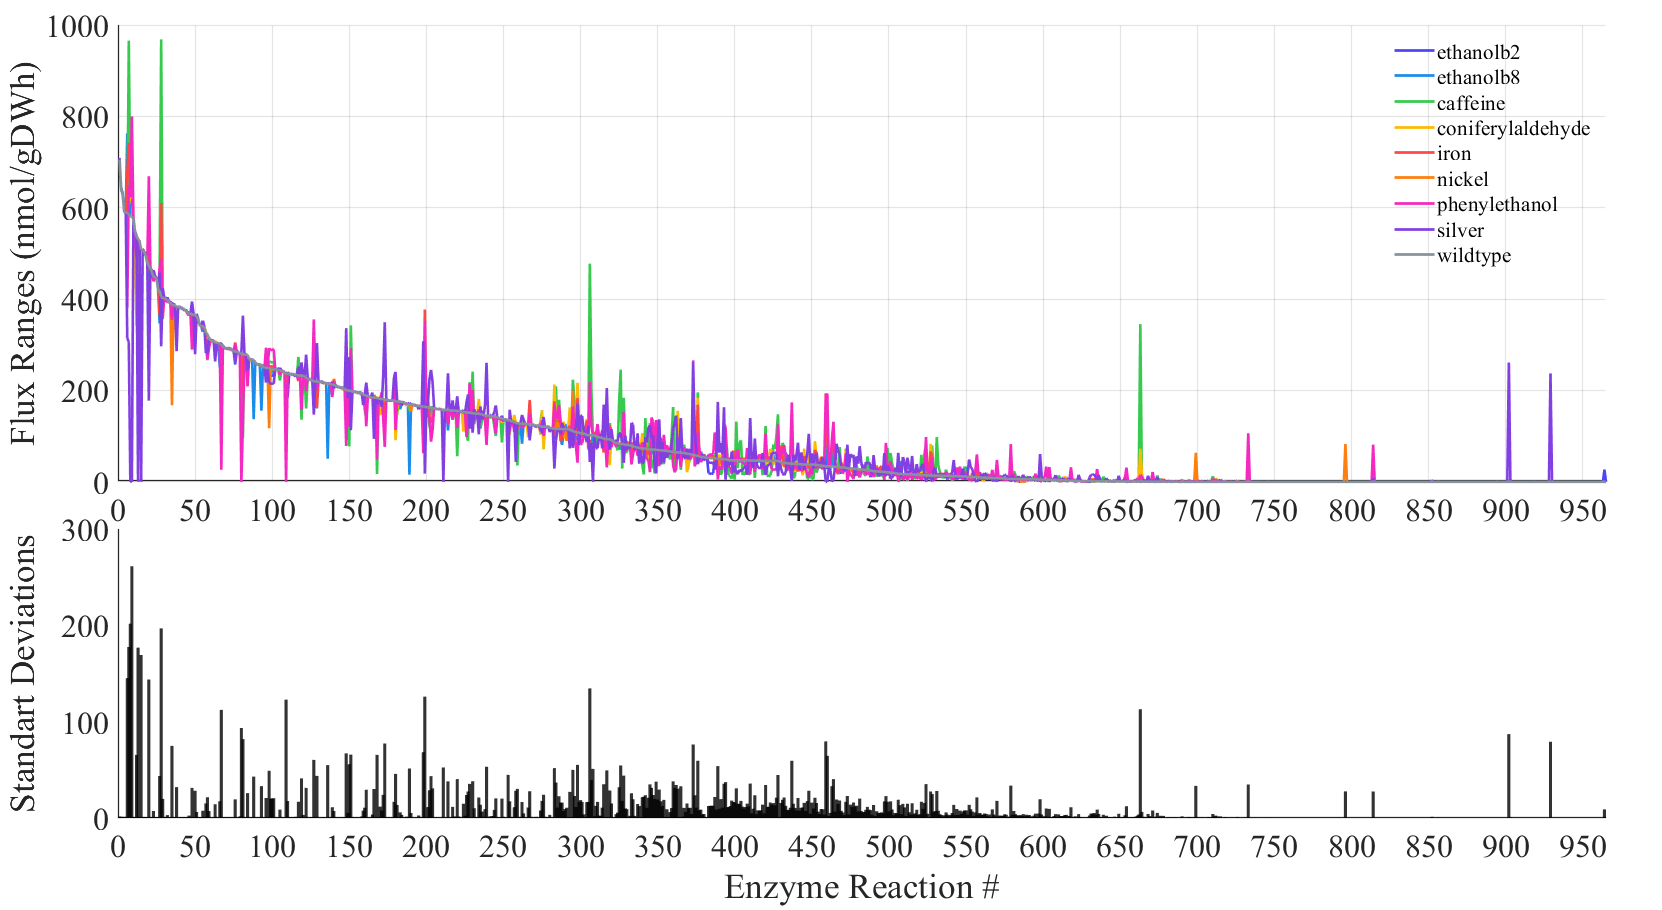
\includegraphics[width=1\columnwidth]{figures/fva_enzymes.png}
  \caption[Flux variability analysis results as flux ranges per enzyme usage reaction, sorted by the wild-type flux ranges]{Flux variability analysis results as flux ranges per enzyme usage reaction, sorted by the wild-type flux ranges.}
  \end{center}
  \label{fig:fva_enzymes}
  \end{figure}

As it can be seen in the Table \ref{table:fva_results} where the most divergent proteins (std $>$ 50) across all experiments are listed, paralog components of the glutathione system namely glutaredoxin-1 (GRX1) and glutaredoxin-2 (GRX2) shows the highest divergence across strains, followed by the glyceraldehyde-3-phosphate dehydrogenase (GAPDH) isozymes, triose-phosphate dehydrogenase 2 and 3 (TDH3 and TDH2).

\begin{table}[H]
\footnotesize
\caption[The most (std $>$ 55 nmol/gDWh) divergent proteins across all experiments and their flux variabilities as ranges (max - min flux) in nmol/gDWh]{The most (std $>$ 55 nmol/gDWh) divergent proteins across all experiments and their flux variabilities as ranges (max - min flux) in nmol/gDWh.}
\vspace{0.3cm}
\begin{center}
  \setlength{\tabcolsep}{4pt}
  \resizebox{\textwidth}{!}{
  \begin{tabular}{|c|c|c|c|c|c|c|c|c|c|c|}
    \hline
\textbf{Enzyme} & \textbf{b2-ethanol} & \textbf{b8-ethanol} & \textbf{caffeine} & \textbf{\begin{tabular}[c]{@{}l@{}}coniferyl \\ aldehyde\end{tabular}} & \textbf{iron} & \textbf{nickel} & \textbf{\begin{tabular}[c]{@{}l@{}}phenyl \\ ethanol\end{tabular}} & \textbf{silver} & \textbf{reference} & \textbf{std} \\ \hline

%
GRX1            & 580.52             & 798.71             & 796.91            & 799.92                     & 799.02        & 580.52          & 799.86                 & 0               & 580.52            & 261.34       \\ \hline
GRX2            & 580.52             & 580.52             & 622.01            & 624.36                     & 623.65        & 580.52          & 622.86                 & 0.08            & 580.52            & 201.73       \\ \hline
TDH3            & 561.29             & 609.88             & 968.54            & 403.74                     & 610.11        & 404.14          & 488.51                 & 296.71          & 403.66            & 196.83       \\ \hline
TDH2            & 702.15             & 760.74             & 965.83            & 607.13                     & 742.34        & 584.58          & 649.07                 & 305.09          & 586.70            & 177.49       \\ \hline
HYR1            & 530.62             & 530.44             & 529.25            & 531.24                     & 530.65        & 531.78          & 529.97                 & 0               & 531.14            & 176.88       \\ \hline
GPX1            & 507.66             & 507.49             & 506.35            & 508.26                     & 507.69        & 508.74          & 507.04                 & 0               & 508.16            & 169.23       \\ \hline
TDH1            & 704.05             & 762.80             & 542.42            & 606.64                     & 672.41        & 586.16          & 381.54                 & 315.49          & 588.29            & 145.14       \\ \hline
OLI1            & 498.12             & 447.32             & 256.85            & 462.14                     & 503.37        & 480.46          & 668.93                 & 177.89          & 471.85            & 143.72       \\ \hline
TRX2            & 83.56              & 76.81              & 477.59            & 85.43                      & 91.79         & 101.72          & 218.84                 & 43.53           & 102.17            & 134.54       \\ \hline
SOL4            & 239.80             & 324.14             & 363.99            & 365.53                     & 377.35        & 156.46          & 351.92                 & 18.15           & 164.11            & 126.02       \\ \hline
ERG10           & 237.06             & 236.98             & 0.01              & 0.02                       & 0.02          & 214.75          & 0.01                   & 238.31          & 237.27            & 122.94       \\ \hline
CYC7            & 3.07               & 6.00               & 345.15            & 72.74                      & 10.38         & 1.24            & 15.25                  & 0.07            & 0.55              & 112.84       \\ \hline
AYR1            & 274.31             & 301.45             & 301.68            & 63.66                      & 301.41        & 301.16          & 26.45                  & 302.96          & 301.69            & 112.20       \\ \hline
PGA3            & 280.31             & 280.22             & 279.59            & 280.28                     & 280.33        & 280.16          & 0                      & 281.75          & 280.59            & 93.47        \\ \hline
SNO3            & 0                  & 0                  & 0                 & 0                          & 0             & 0               & 0                      & 261.32          & 0                 & 87.11        \\ \hline
DAS2            & 259.51             & 224.29             & 96.71             & 211.09                     & 191.35        & 276.99          & 126.60                 & 363.82          & 279.13            & 81.82        \\ \hline
HXK1            & 82.23              & 146.33             & 188.50            & 189.24                     & 193.89        & 33.59           & 186.56                 & 0.01            & 34.44             & 79.54        \\ \hline
SNO2            & 0                  & 0                  & 0                 & 0                          & 0             & 0               & 0                      & 237.53          & 0                 & 79.18        \\ \hline
URA6            & 153.11             & 148.21             & 113.37            & 133.15                     & 123.92        & 175.63          & 76.48                  & 349.32          & 179.93            & 77.32        \\ \hline
YDC1            & 265.82             & 137.27             & 265.96            & 265.85                     & 265.50        & 265.13          & 265.98                 & 261.85          & 58.55             & 76.34        \\ \hline
YOR283W         & 385.25             & 284.27             & 374.59            & 386.44                     & 383.88        & 167.70          & 354.85                 & 391.22          & 387.67            & 74.91        \\ \hline
SOL3            & 173.27             & 160.34             & 102.97            & 127.45                     & 116.01        & 161.25          & 62.84                  & 307.74          & 165.03            & 68.26        \\ \hline
CDC8            & 180.45             & 172.85             & 222.25            & 182.36                     & 168.37        & 198.14          & 78.50                  & 336.56          & 201.04            & 67.03        \\ \hline
ALG13           & 222.59             & 233.87             & 342.51            & 266.53                     & 268.81        & 198.78          & 292.49                 & 113.05          & 199.23            & 65.73        \\ \hline
GPX2            & 537.40             & 537.23             & 536.02            & 341.26                     & 537.43        & 538.58          & 488.86                 & 540.21          & 537.93            & 65.52        \\ \hline
PDC5            & 157.75             & 161.29             & 17.12             & 185.99                     & 76.60         & 181.67          & 48.37                  & 169.86          & 183.92            & 65.47        \\ \hline
GLK1            & 27.76              & 50.03              & 133.67            & 135.09                     & 92.54         & 33.06           & 193.48                 & 0               & 34.35             & 64.44        \\ \hline
GPP2            & 204.17             & 215.88             & 261.44            & 299.76                     & 230.49        & 212.94          & 355.61                 & 147.19          & 219.99            & 60.29        \\ \hline
ALD4            & 44.53              & 37.53              & 140.64            & 138.00                     & 78.24         & 40.30           & 174.06                 & 1.32            & 39.86             & 59.43        \\ \hline
PYK2            & 91.09              & 88.38              & 195.97            & 183.93                     & 169.19        & 55.15           & 108.01                 & 38.43           & 56.16             & 59.39        \\ \hline
ALG14           & 179.10             & 169.99             & 77.84             & 142.43                     & 140.31        & 198.78          & 120.83                 & 273.04          & 199.23            & 55.73        \\ \hline
MHT1            & 107.29             & 91.30              & 170.34            & 216.78                     & 183.08        & 108.03          & 41.78                  & 171.04          & 108.32            & 55.14        \\ \hline

\end{tabular}}
\label{table:fva_results}
\end{center}
\end{table}


Pathway-wise investigation is carried out from the flux variability analysis results. First, the reactions that have subsystem annotations are collected for each seperately. It must be noted that some reactions can exist in multiple subsystems, for example, phosphoenolpyruvate carboxykinase reaction exists in all gluconeogenesis, glycolysis, citrate cycle (TCA cycle), pyruvate metabolism, biosynthesis of secondary metabolites, biosynthesis of antibiotics, and carbon metabolism subsystems. Secondly, the mean flux values for each subsystem for all models in flux variability analysis are collected. These flux values for the most common subsystems are plotted as stacked bars in Figure \ref{fig:fva_subsystem_spans} to distinguish subsystem activity for each model after the normalization arised from the assumption of the total flux value for each model should be equal in order to allow comparison.

\begin{figure}[H]
  \begin{center}
  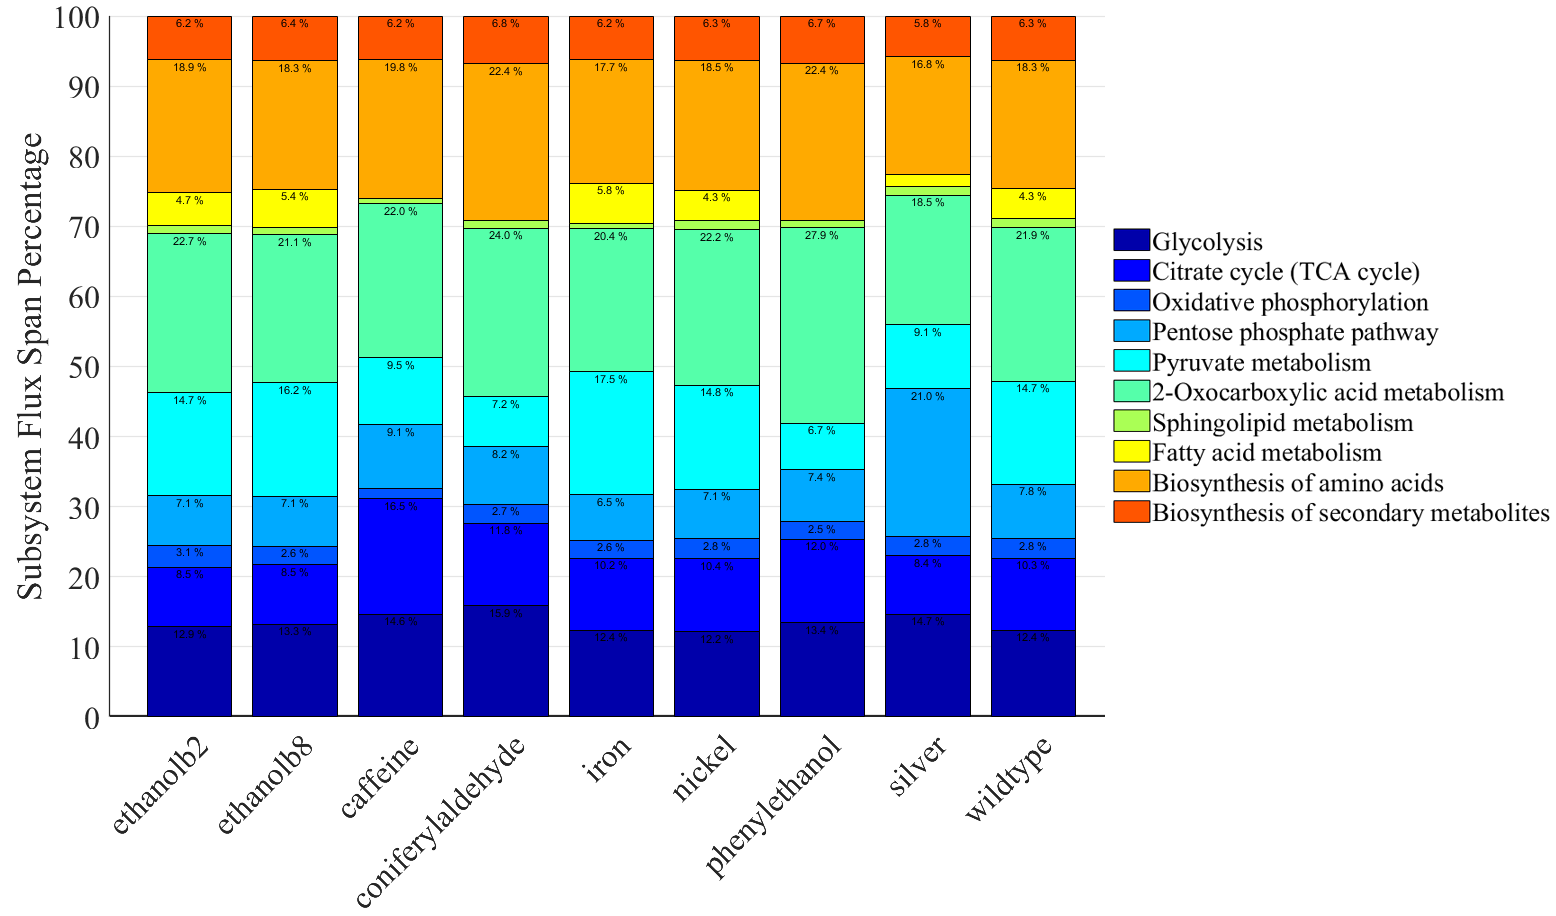
\includegraphics[width=1\columnwidth]{figures/fva_subsystem_spans.png}
  \caption[Mean carried fluxes through the ubsystems are shown as stacked bars for strain-wise comparison. Sum of fluxes are normalized to a hundred percent to be able to distinguish flux distribution]{Mean carried fluxes through the ubsystems are shown as stacked bars for strain-wise comparison. Sum of fluxes are normalized to a hundred percent to be able to distinguish flux distribution.}
  \label{fig:fva_subsystem_spans}
  \end{center}
\end{figure}

Despite the similarities in the flux values some of the subsystems, interesting results are observed. The most distinguished models are observed as caffeine, coniferylaldehyde and phenylethanol strains as they do not carry fluxes through fatty acid metabolism reactions. Instead, the caffeine model shows higher activity in the TCA cycle reactions, compared to coniferylaldehyde and phenylethanol strains where the activity increases in the 2-oxocarboxylic acid metabolism.

\section{Survivability Analysis: Knock-out Simulations}
To calculate the essentiality of the reactions and the proteins on the growth, \emph{in-silico} single deletion analyses are done on all the reactions for each model. Growth rate ratios between deletion applied models and the prior models are collected as percentages for each strain. The reactions that have the same value for each experiment are discarded from the results considering they do not differ after evolution. To be able to catch the most important proteins, only the reactions with the minimum of \%95 growth rate decreases are reported here. The impacts of the deleted reactions are seperately shown as heatmaps in Figure \ref{fig:deletion_survivability_rxns} for metabolic reactions and in Figure \ref{fig:deletion_survivability_prots} proteins.

\begin{figure}[H]
  \begin{center}
  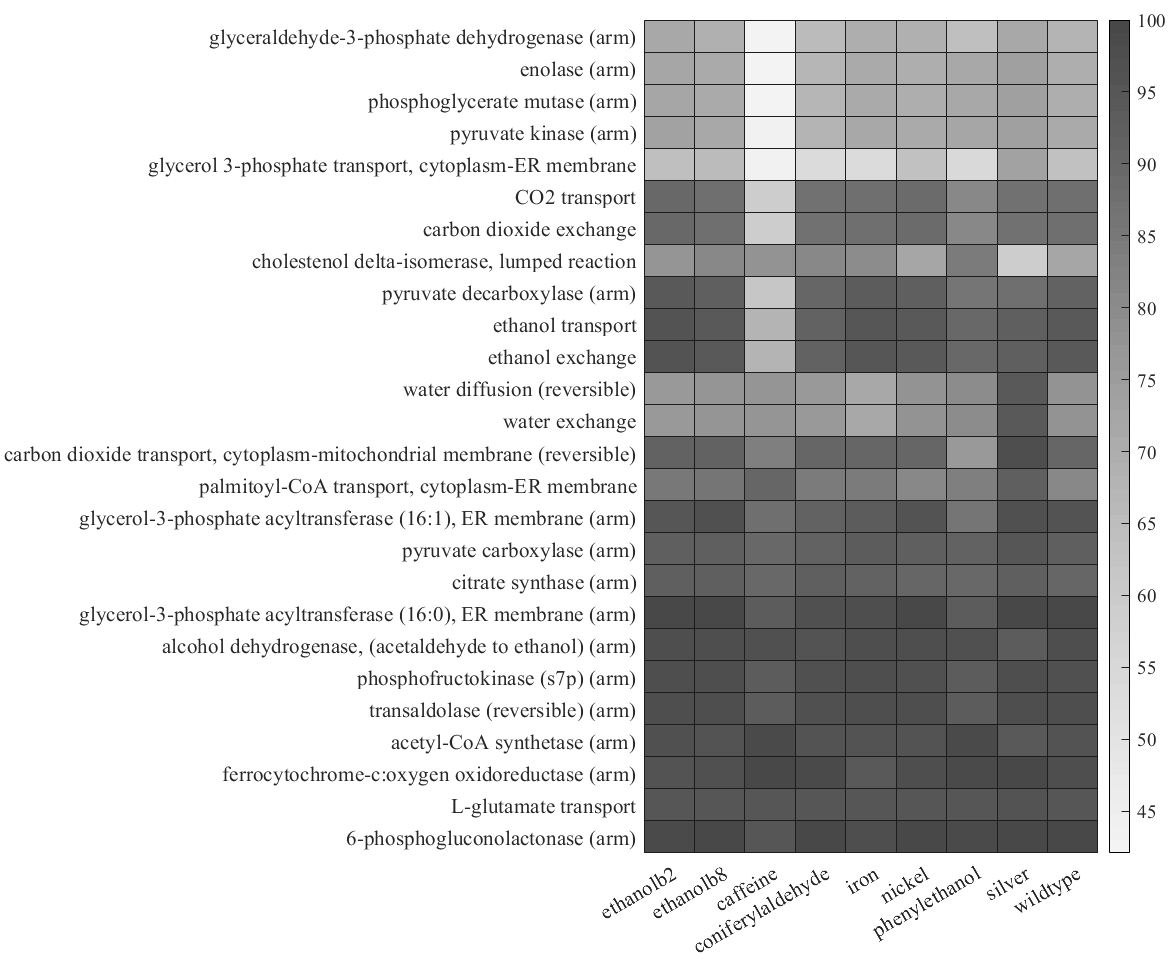
\includegraphics[width=1\columnwidth]{figures/deletion_survivability_rxns.png}
  \caption[Heatmaps of the growth rate ratios between deletion strains for each experiment. The knocked-out reactions that cause a decrease higher than \%95 are reported.]{Heatmaps of the growth rate ratios between deletion strains for each experiment. The knocked-out reactions that cause a decrease higher than \%95 are reported.}
  \label{fig:deletion_survivability_rxns}
  \end{center}
\end{figure}

\begin{figure}[H]
  \begin{center}
  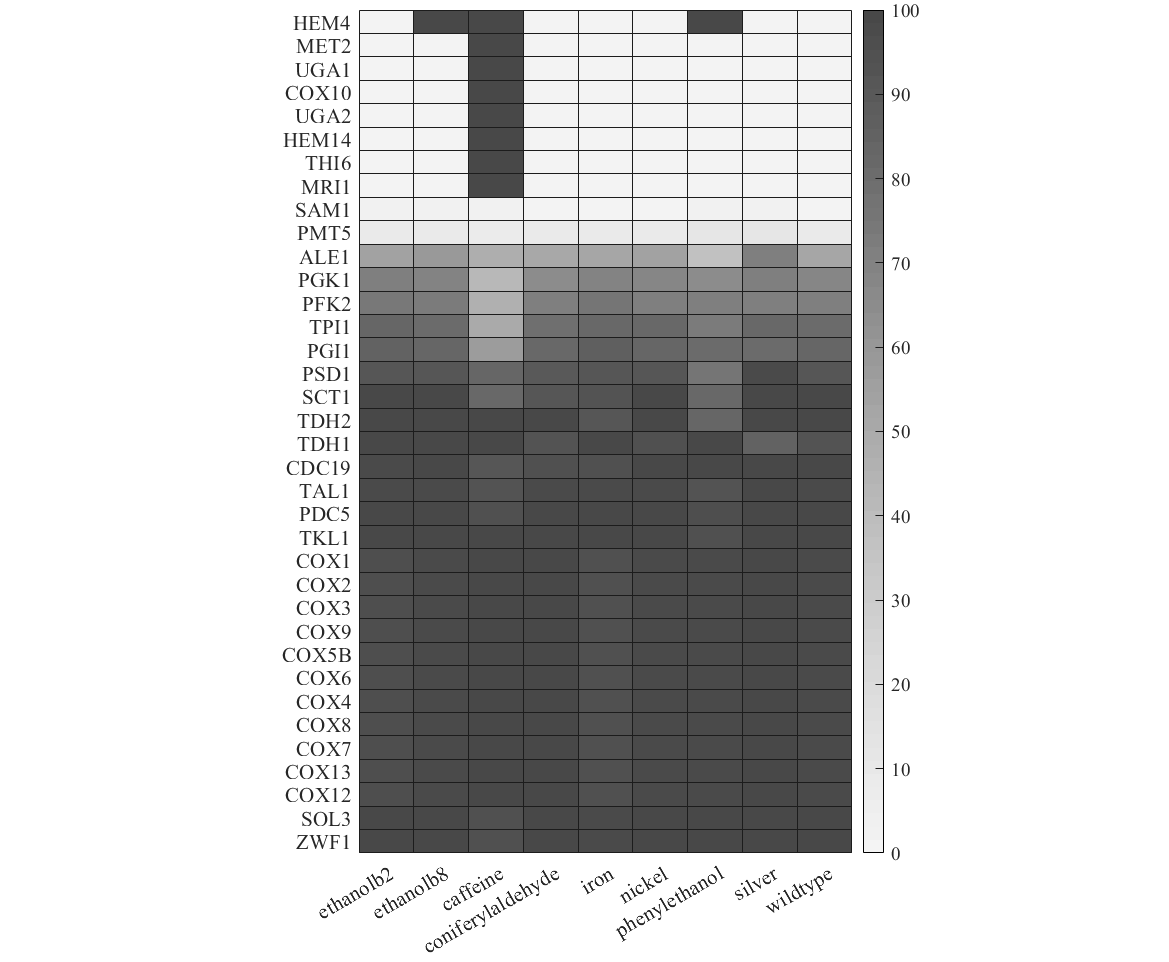
\includegraphics[width=1\columnwidth]{figures/deletion_survivability_prots.png}
  \caption[Heatmaps of the growth rate ratios between deletion strains for each experiment. The knocked-out proteins that cause a decrease higher than \%95 are reported.]{Heatmaps of the growth rate ratios between deletion strains for each experiment. The knocked-out proteins that cause a decrease higher than \%95 are reported.}
  \label{fig:deletion_survivability_prots}
  \end{center}
\end{figure}

Although all the models were able to grow in any single deletion on the reactions (with the minimum 45\% lower growth rate from the non-deletion models), 2 enzymes (SAM1 and PMT5) are found essential for all models. Interestingly, MET2, UGA1, COX10, UGA2, HEMI4, THI6 and MRI1 enzymes were essential for all models except the caffeine-resistant model. On the other hand, the deletion of the PGK1, PFK2, TPI1 and PFI1 enzymes decreases the caffeine-resistant model's growth ability higher than other models.

\section{Minimization of Metabolic Adjustment}

Minimization of metabolic adjustment (MOMA) analysis is applied to evolved models to find the closest points to wild-type model simulations (in terms of the Euclidean distances). Analysis is done with the objective of maximization of the growth rate and no constraints applied to the models except for the total protein amount availability. Results are collected for the metabolic reactions and the proteins (as enzyme-draw reactions) seperately. The sum of the distances from the wildtype simulations is used as a ranking system to find most distant reactions and proteins. Individual fluxes through reactions can be seen in Figure \ref{fig:moma_cumdist}.


 The most distant reactions in the evolved models from the wild type model found as palmitoyl-CoA hydrolase, followed by the long chain fatty acid CoA ligase, deoxyuridine kinase, methylglyoxal synthase, 5' nucleotidases, glutathione metabolism reactions. On the other hand, the enzymes TDH1 (glyceraldehyde-3-phosphate dehydrogenase isozyme 1), OLI1 (F0 ATP synthase subunit c), GPT2 (glycerol-3-phosphate/dihydroxyacetone phosphate sn-1 acyltransferase), RIB7 (Diamino-hydroxy-phoshoribosyl-amino-pyrimidine deaminase), SCT1 (glycerol 3-phosphate/dihydroxyacetone phosphate sn-1 acyltransferase) and COB (cytochrome b) were the top distant enzymes in terms of enzyme-draw reaction fluxes.

\begin{figure}[H]
  \begin{center}
  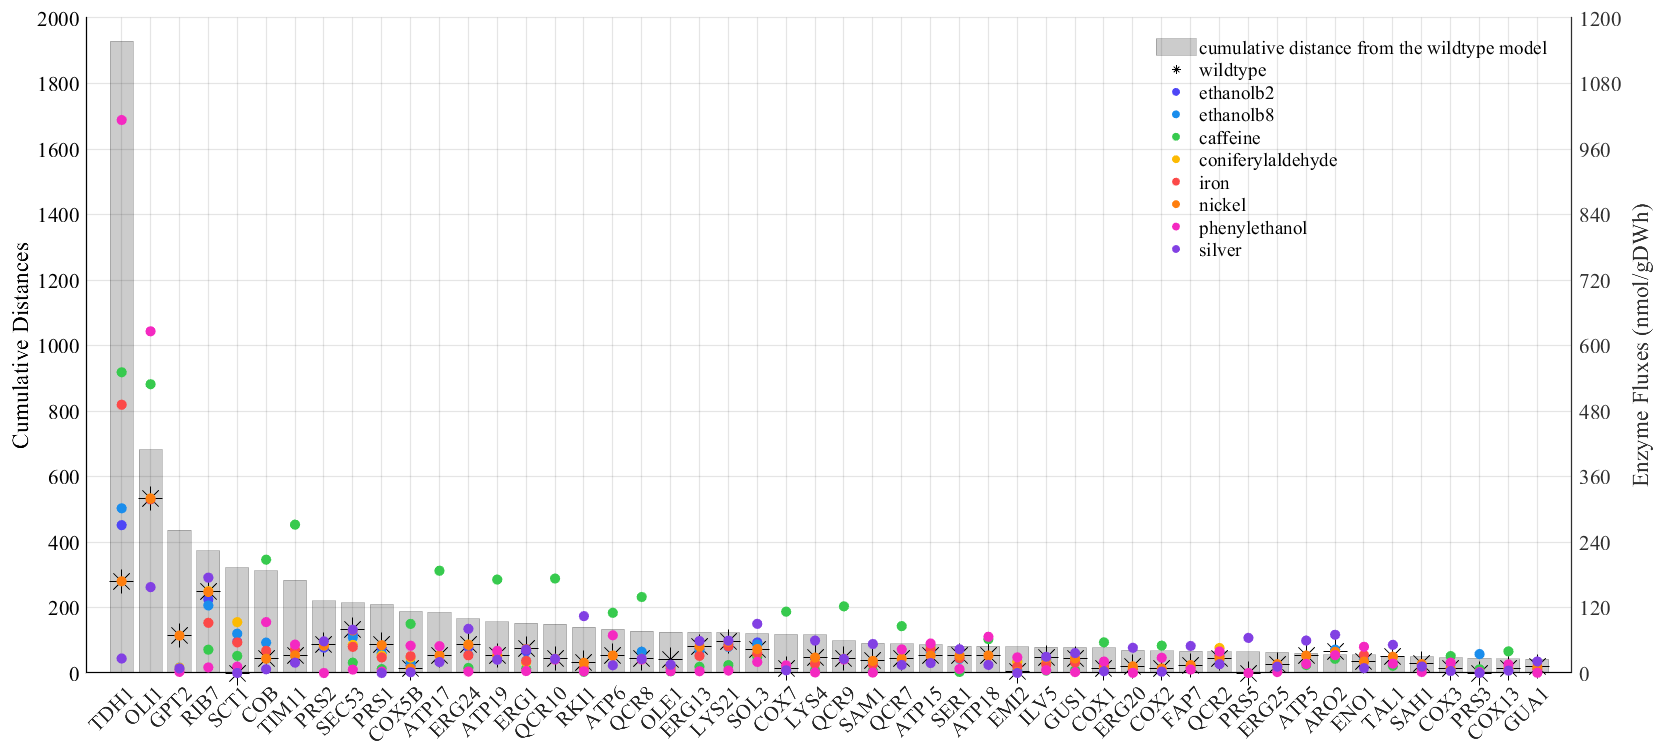
\includegraphics[width=1\columnwidth]{figures/moma_cumdist.png}
  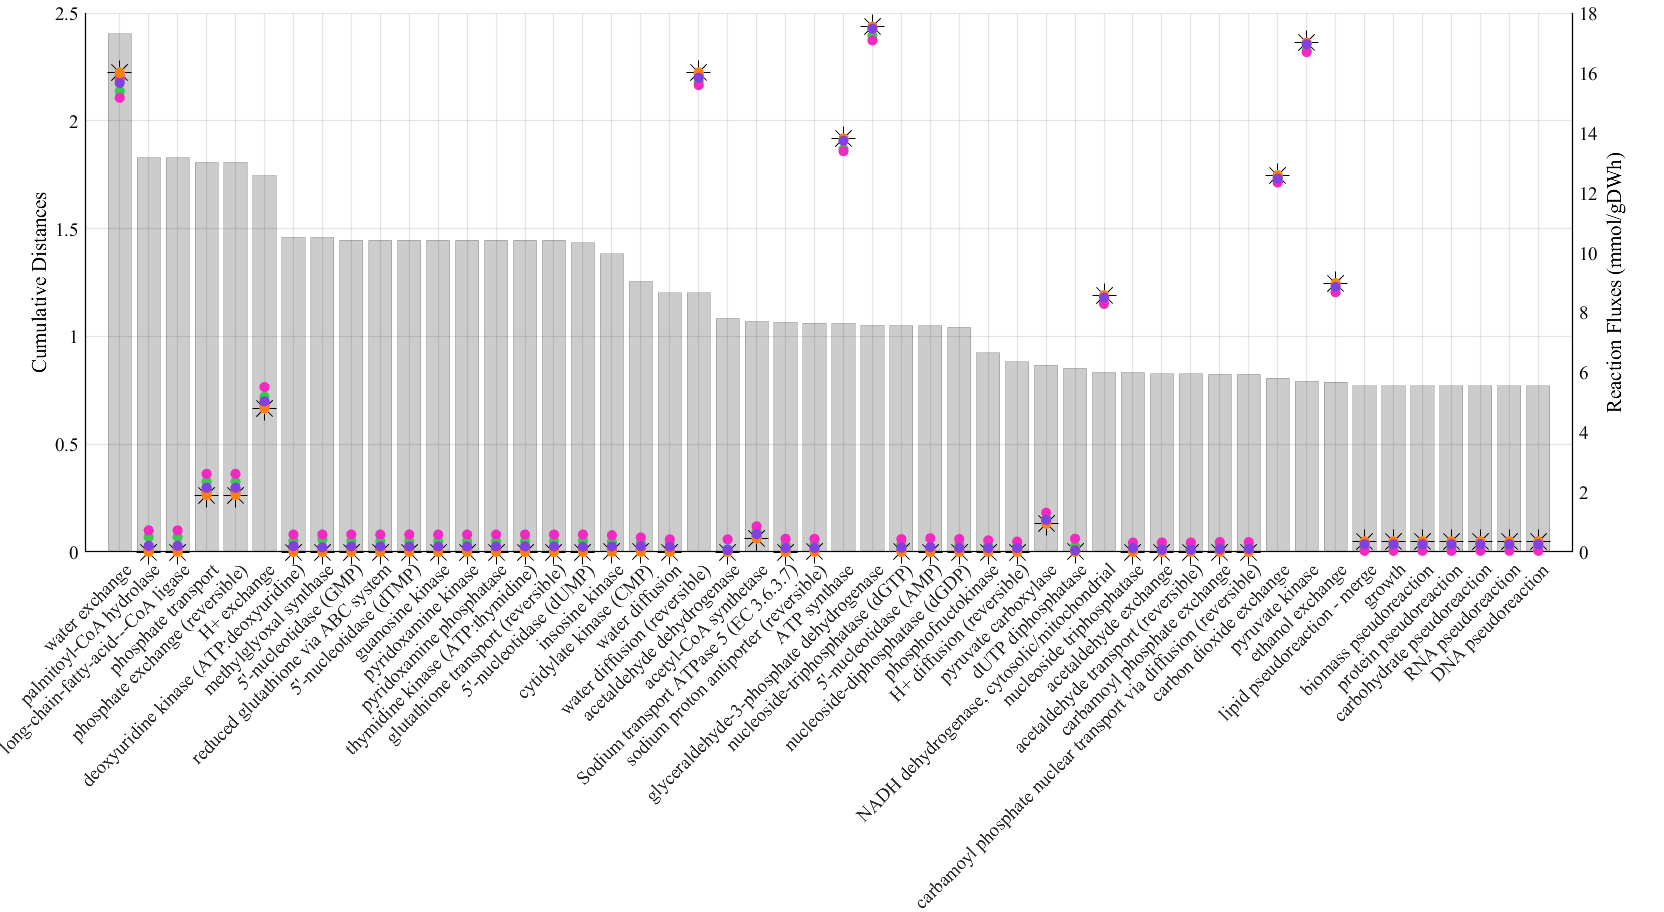
\includegraphics[width=1\columnwidth]{figures/moma_cumdist_rxns.png}
  \caption[Enzymes that have MOMA flux values the most distant from the wild-type flux values in nmol/gDWh]{Enzymes that have MOMA flux values the most distant from the wild-type flux values in nmol/gDWh.}
  \label{fig:moma_cumdist}
  \end{center}
\end{figure}

\section{Sampling Results}

The random solutions for each metabolic models are obtained by maximizing  for a random set of three reactions with random weights. Total of 10,000 solutions for each model are generated after the boundaries on growth rate as an objective function is set to minimum of 90\% and maximum of 100\% growth rate of the flux balance analysis results. The solution spaces for these reactions are plotted as histogram plots where the bin counts, N, are normalized so that the sum(N) is 1 for each analysis.

The most divergent reactions excluding diffusion, transport and exchange reactions from FBA results are plotted in Figure \ref{fig:sampling_fba_top12}, the most divergent enzymes from FVA results are plotted in Figure \ref{fig:sampling_fva_top12}, followed by the MOMA hits in Figure \ref{fig:sampling_moma_top12}.

\begin{figure}[H]
  \begin{center}
  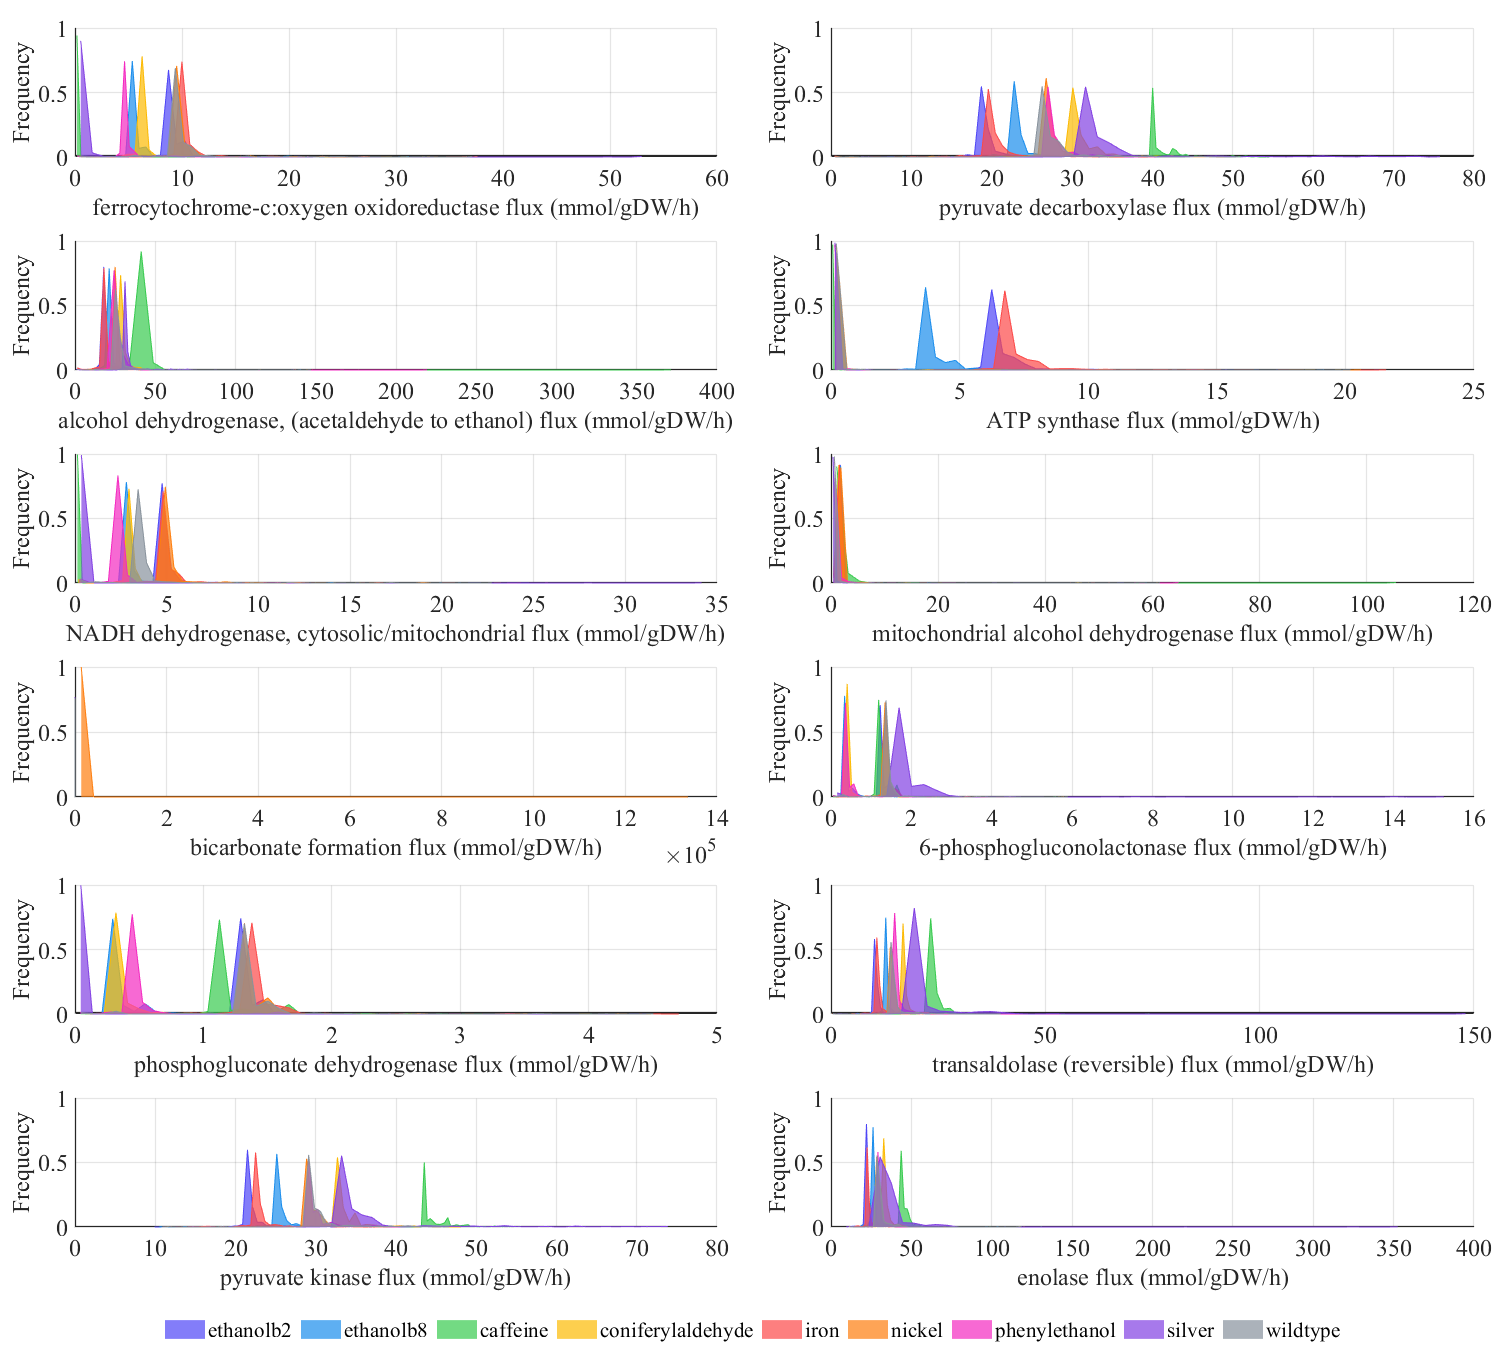
\includegraphics[width=1\columnwidth]{figures/sampling_fba_top12.png}
  \caption[Flux distributions of the reactions that diverge the most in flux balance analysis, obtained from the random sampling of solution spaces for each model shown as histogram plots]{Flux distributions of the reactions that diverge the most in flux balance analysis, obtained from the random sampling of solution spaces for each model shown as histogram plots.}
  \label{fig:sampling_fba_top12}
  \end{center}
\end{figure}

Ferrocytochrome-c:oxygen oxidoreductase reaction shows a great divergence across all models despite having the 0 flux on the caffeine resistant model. This 0 flux on the caffeine model explains the higher fluxes through alcohol dehydrogenase reaction, meaning thet the oxidative phosphorylation rates are lower in the caffeine resistant model compared to ethanol producing pathways. Pyruvate decarboxylase reaction shows almost the pattern with the pyruvate kinase reaction indicating a chain reaction. Remember that the although the models are fed with the same amount of carbon sources, small differences in their reaction fluxes comes from the adaptive evolution expression analyses. That reminded, the small flux values on the 6-phosphogluconolactonase reaction biologically may not mean a big difference, however the different behavior of the silver resistant model (having a wider range over other models) could mean the availability of the althernative pathways for the same biological objective.


\begin{figure}[H]
  \begin{center}
  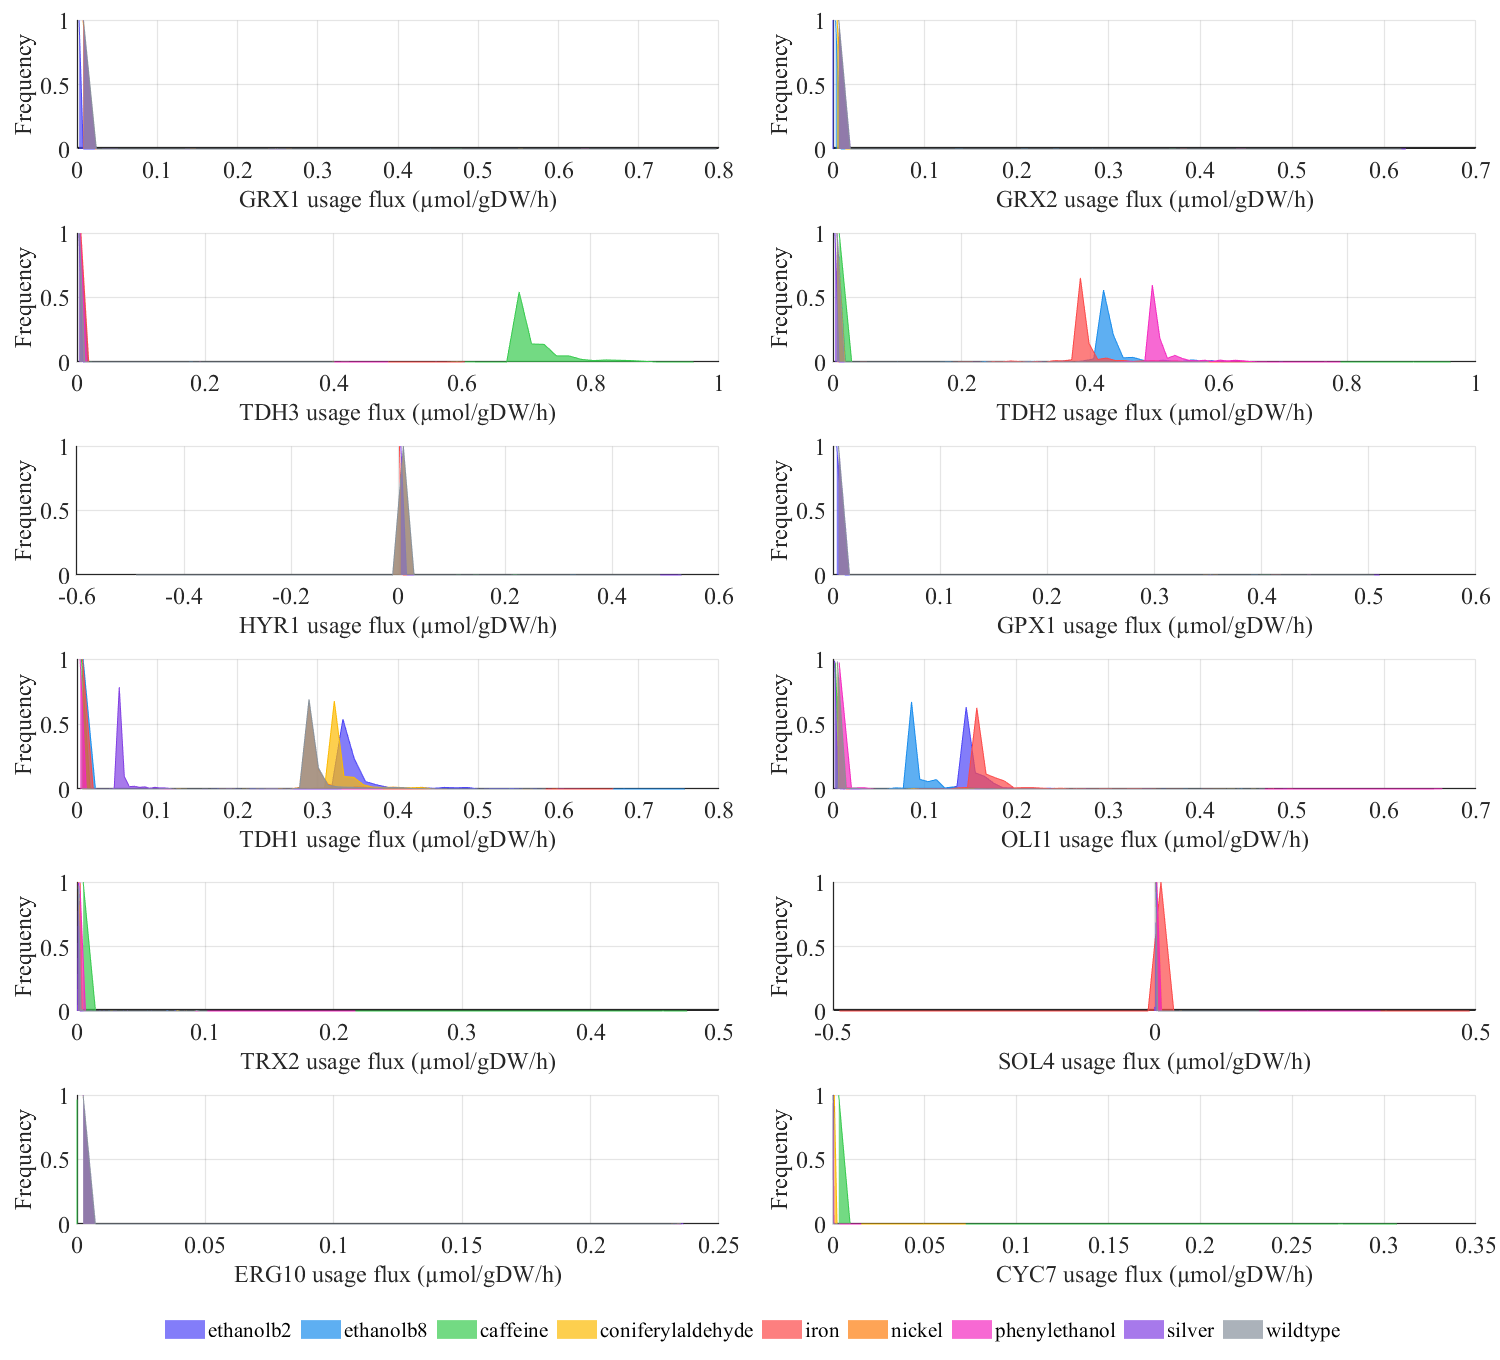
\includegraphics[width=1\columnwidth]{figures/sampling_fva_top12.png}
  \caption[Flux distributions of the reactions that diverge the most in flux variability analysis, obtained from the random sampling of solution spaces for each model shown as histogram plots]{Flux distributions of the reactions that diverge the most in flux variability analysis, obtained from the random sampling of solution spaces for each model shown as histogram plots.}
  \label{fig:sampling_fva_top12}
  \end{center}
\end{figure}

Enzyme fluxes are numerically hard to distinguish in histogram plots because of the lower magnitude of the enzyme kinetics. The main target enzymes from the flux variability analysis are found as the glutaredoxin paralogs (GRX1 and GRX2) mostly did not show a very different behaviors on the sampled solution spaces. Glyceraldehyde-3-phosphate dehydrogenase isozymes (TDH1, TDH2 and TDH3) on the other hand show the different preferences between models.

In order to investigate enzyme relationships, correlation coefficients for each enzyme is calculated from the solution spaces for all models. Considering only the correlation values higher than R $>$ 0.5, GRX enzymes are found to be positively correlated with the phospholipid hydroperoxide glutathione peroxidase (GPX) enzymes (Figure \ref{fig:sampling_correlation_grx}).

\begin{figure}[H]
  \begin{center}
  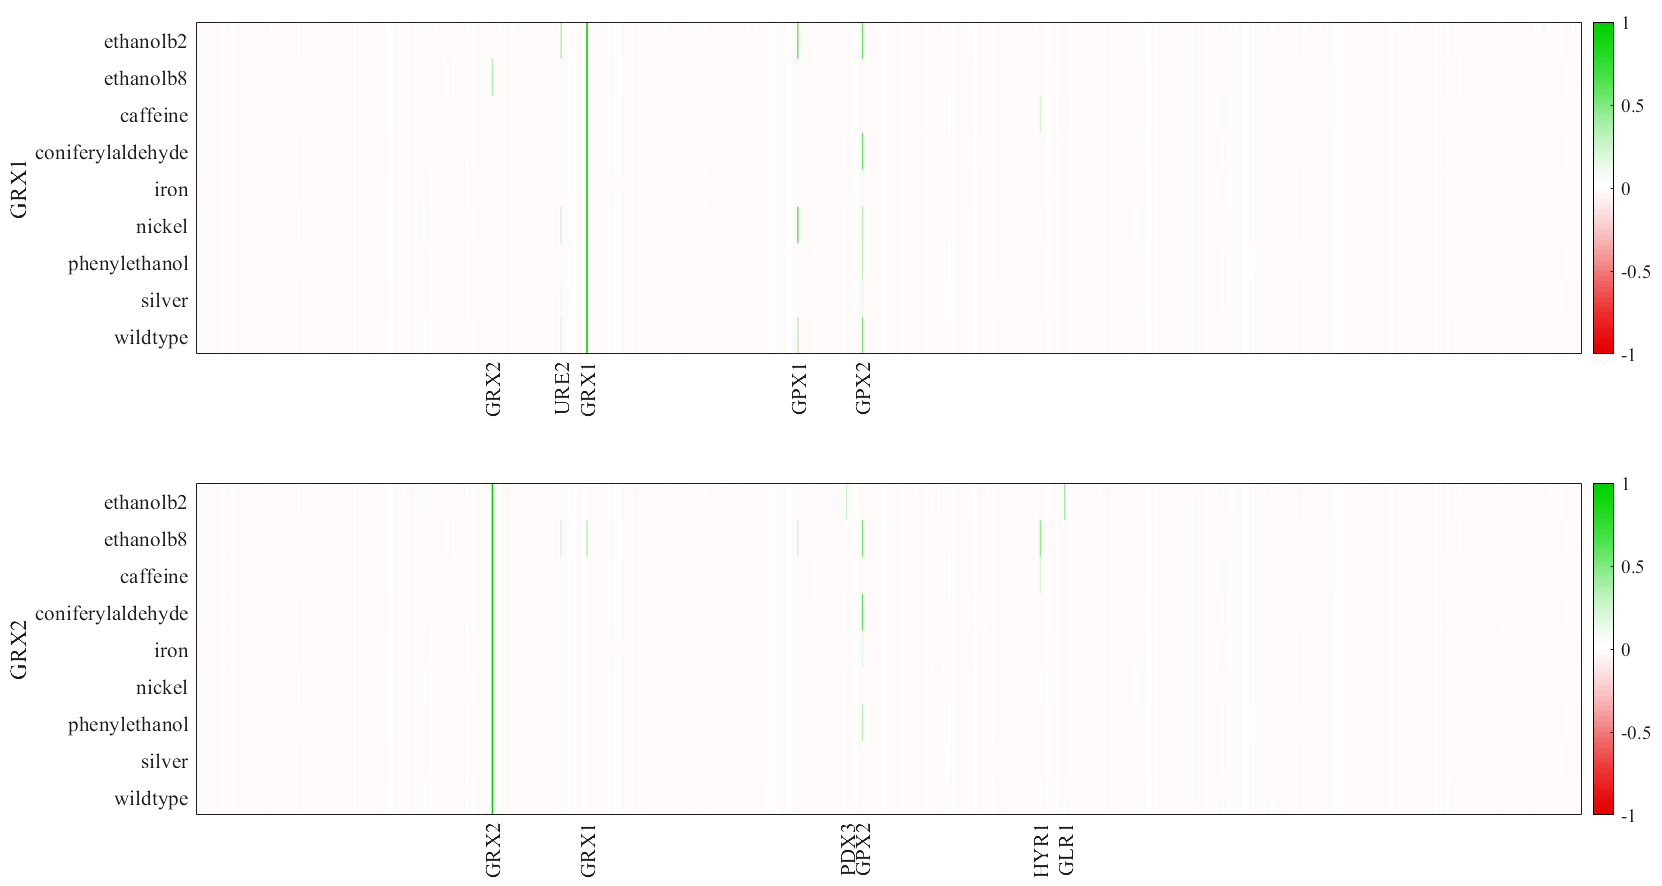
\includegraphics[width=1\columnwidth]{figures/sampling_correlation_grx.png}
  \caption[Correlations of GRX1 (top) and GRX2 (bottom) enzymes to other enzymes calculated from the random sampling of solution spaces. Only the name of enzymes with the correlation value c$>$0.8 are shown in the y-axes]{Correlations of GRX1 (top) and GRX2 (bottom) enzymes to other enzymes calculated from the random sampling of solution spaces. Only the name of enzymes with the correlation value c$>$0.3 are shown in the y-axes}
  \label{fig:sampling_correlation_grx}
  \end{center}
\end{figure}

TDH3 enzyme shows positive correlation only in the caffeine resistant model to 4 enzymes: An enzyme responsible for the regulation of telomerase (CDC13), minor isoform of pyruvate decarboxylase (PDC5), subunit of phosphofructokinase (PFK2), and to a protein of unknown function (EMI2). TDH1 and TDH3 enzymes on the other hand show both positive and negative correlations to multiple enzymes (Figure \ref{fig:sampling_correlation_tdh}).

\begin{figure}[H]
  \begin{center}
  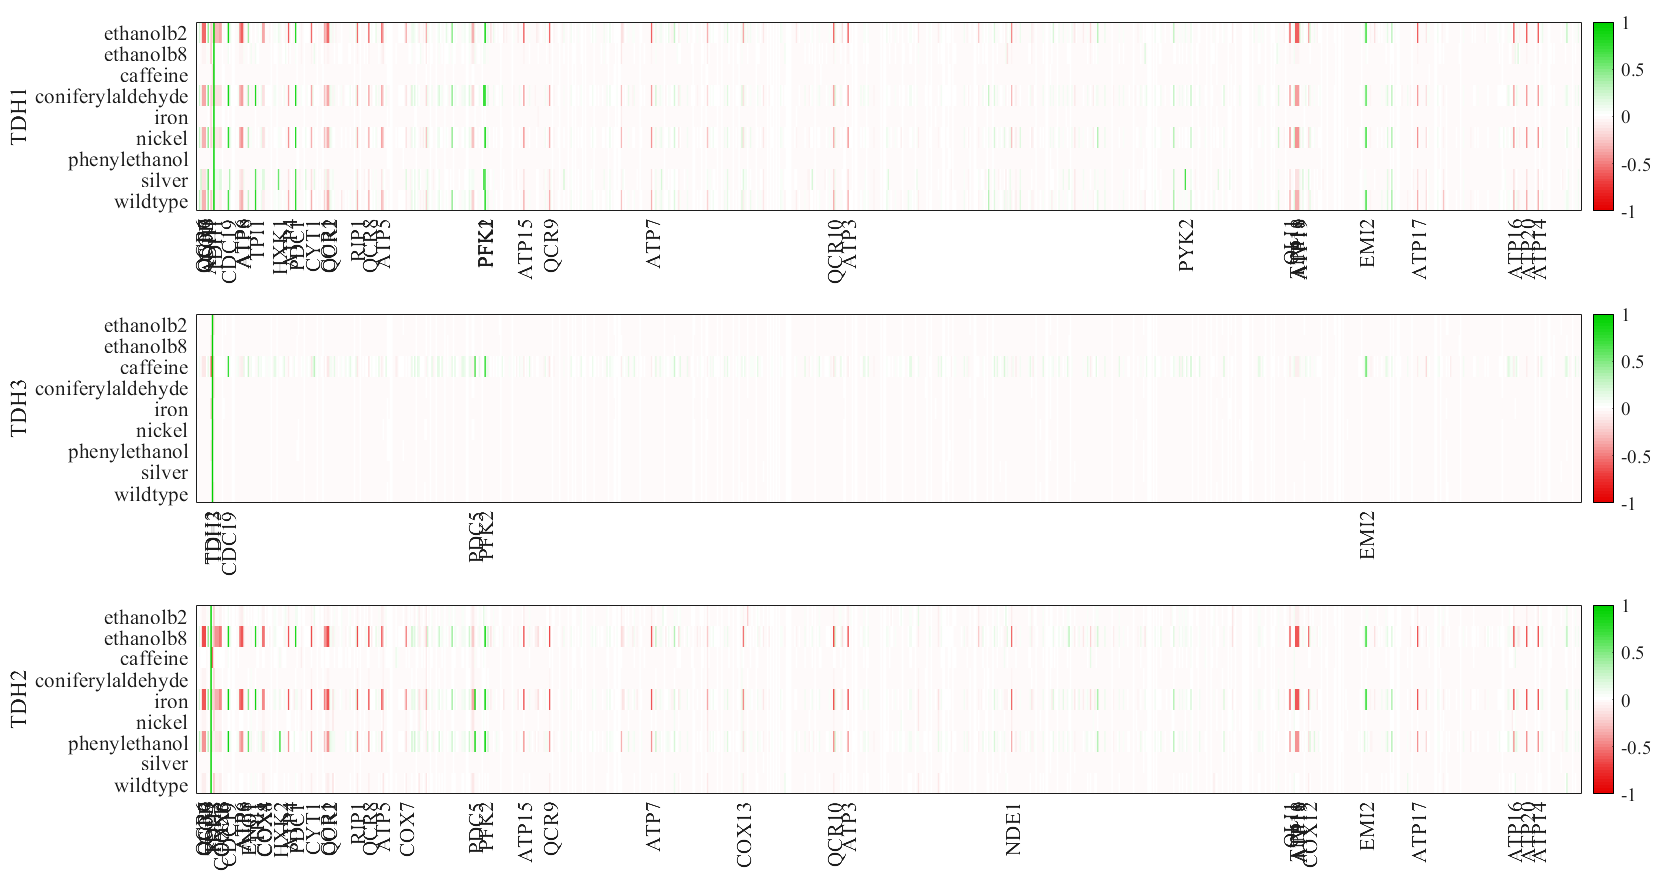
\includegraphics[width=1\columnwidth]{figures/sampling_correlation_tdh.png}
  \caption[Correlations of TDH1 (top), TDH3 (middle) and TDH2 (bottom) enzymes to other enzymes calculated from the random sampling of solution spaces. Only the name of enzymes with the correlation value c$>$0.5 are shown in the y-axes]{Correlations of TDH1 (top), TDH3 (middle) and TDH2 (bottom) enzymes to other enzymes calculated from the random sampling of solution spaces. Only the name of enzymes with the correlation value c$>$0.5 are shown in the y-axes.}
  \label{fig:sampling_correlation_tdh}
  \end{center}
\end{figure}

\begin{figure}[H]
  \begin{center}
  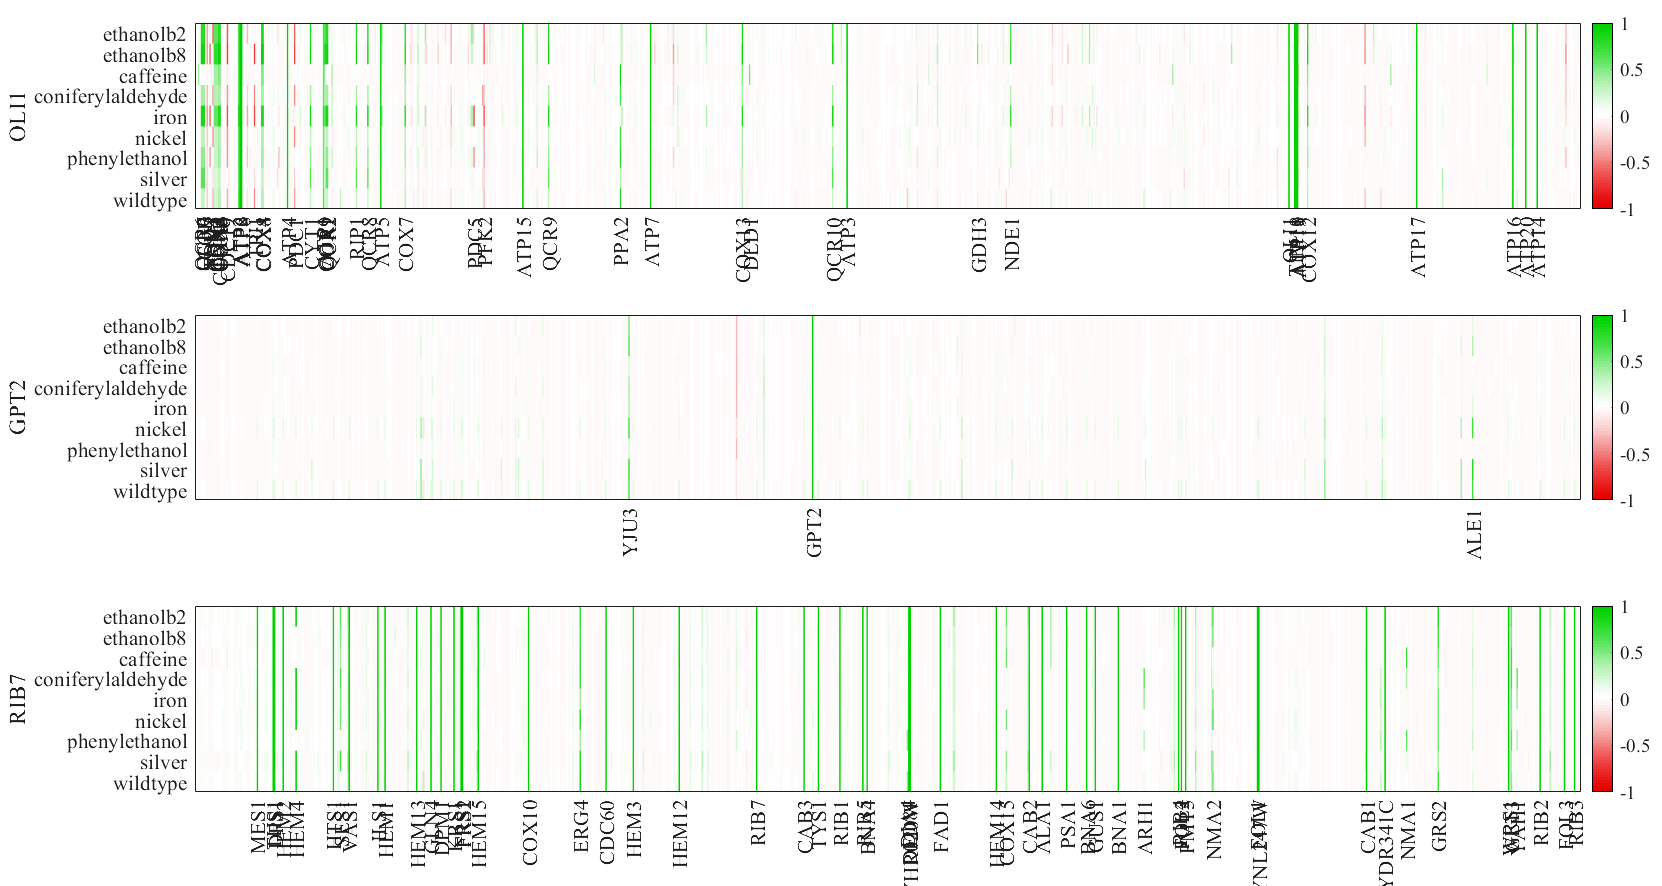
\includegraphics[width=1\columnwidth]{figures/sampling_correlation_oli_gpt_rib.png}
  \caption[Correlations of OLI1 (top), GPT2 (middle) and RIB7 (bottom) enzymes to other enzymes calculated from the random sampling of solution spaces. Only the name of enzymes with the correlation value c$>$0.5 are shown in the y-axes]{Correlations of OLI1 (top), GPT2 (middle) and RIB7 (bottom) enzymes to other enzymes calculated from the random sampling of solution spaces. Only the name of enzymes with the correlation value c$>$0.5 are shown in the y-axes.}
  \label{fig:sampling_correlation_oli_gpt_rib}
  \end{center}
\end{figure}

When we further investigate the enzymatic correlations of OLI1 (F0 ATP synthase subunit c), GPT2 (glycerol-3-phosphate/dihydroxyacetone phosphate sn-1 acyltransferase), and RIB7 (Diamino-hydroxy-phoshoribosyl-amino-pyrimidine deaminase) to other enzymes. We see that RIB7 shows similar results across models with the exception of correlations with HEM4 enzyme (uroporphyrinogen III synthase) absent in ethanolb8, caffeine and phenylethanol resistant models. Similar to HEM4 enzyme, COX15 (heme a synthase), ARH1 (mitochondrial oxidoreductase), NMA1 (nicotinic acid mononucleotide adenylyltransferase) and YAH1 (ferredoxin) enzymes must be investigated since they show different correlations across models although they are all involved in the heme biosynthesis pathways. In the case of OLI1, both positive and negative correlations are observed within all models, although the most distinct strain appears as caffeine resistant model by showying less correlations. GPT2 enzyme positively correlates with YJU3 (monoglyceride lipase) and ALE1 (lysophospholipid acyltransferase) enzymes in wildtype, silver and nickel resistant models with lower correlation values in caffeine resistant model.

\begin{figure}[H]
  \begin{center}
  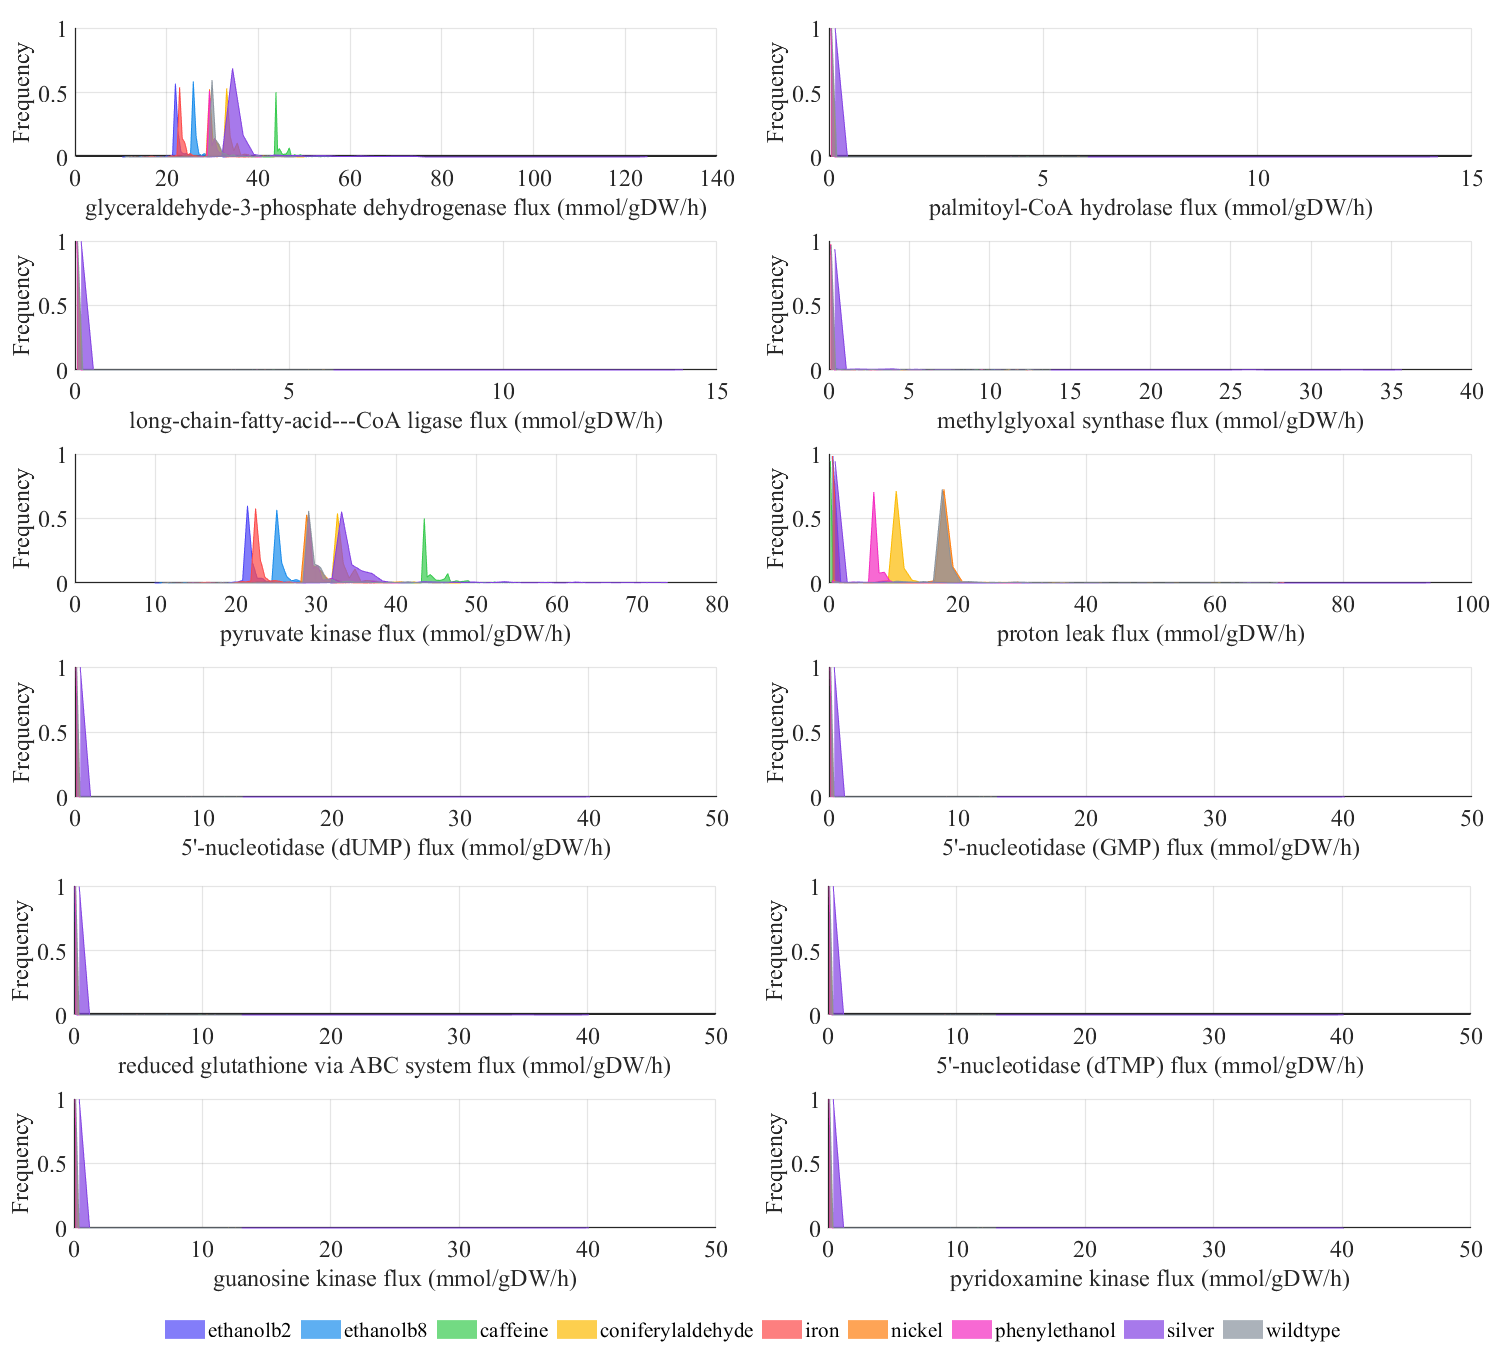
\includegraphics[width=1\columnwidth]{figures/sampling_moma_top12.png}
  \caption[Flux distributions of the reactions that diverge the most in the minimization of metabolic adjustment analysis, obtained from the random sampling of solution spaces for each model shown as histogram plots]{Flux distributions of the reactions that diverge the most in the minimization of metabolic adjustment analysis, obtained from the random sampling of solution spaces for each model shown as histogram plots.}
  \label{fig:sampling_moma_top12}
  \end{center}
\end{figure}

Glyceraldehyde-3-phosphate dehydrogenase reaction ranks once again #1 in a different analysis, MOMA. It can be seen that separation is clear in all models with a wider flux range in the silver resistant model meaning that its flux value differ in multiple solutions. Followed by palmitoyl-CoA hydrolase, long chain fatty acid-CoA ligase and methylglyoxal synthase reactions are only in the Figure because they are only active in the silver resistant model. However since their flux ranges are too close to 0, they cannot be investigated as solid foundings. Pyruvate kinase reaction shows the same pattern as in previous analyses. Interestingly, proton leak reaction (leakage of hydrogen atoms from cytoplasm to mitochondria) carries flux up to 20 mmol/gDWh, indicating that in the phenylethanol, coniferylaldehyde and nickel resistant models, more than available proton is required in the mitochondria. Lastly, 5'-nucleotidase reactions, guanosine kinase and pyridoxamine kinase reactions are only active for silver resistant model, same as the previously mentioned reactions.

Finally, mean values for each enzyme from solution spaces are calculated. Z-scores are obtained from the difference between this means in each strain model to the wildtype model fluxes, divided by
the square root of the sum of standard deviations of this difference. Z-scores for enzymes are converted to p-values within gaussian distribution, and compared to the p-values obtained from the differential expression analysis. Discarding the non-significant enzymes in both cases, the following Figure \ref{fig:sampling_regulation_heatmaps} is constructed to compare regulations.

\begin{figure}[H]
  \begin{center}
  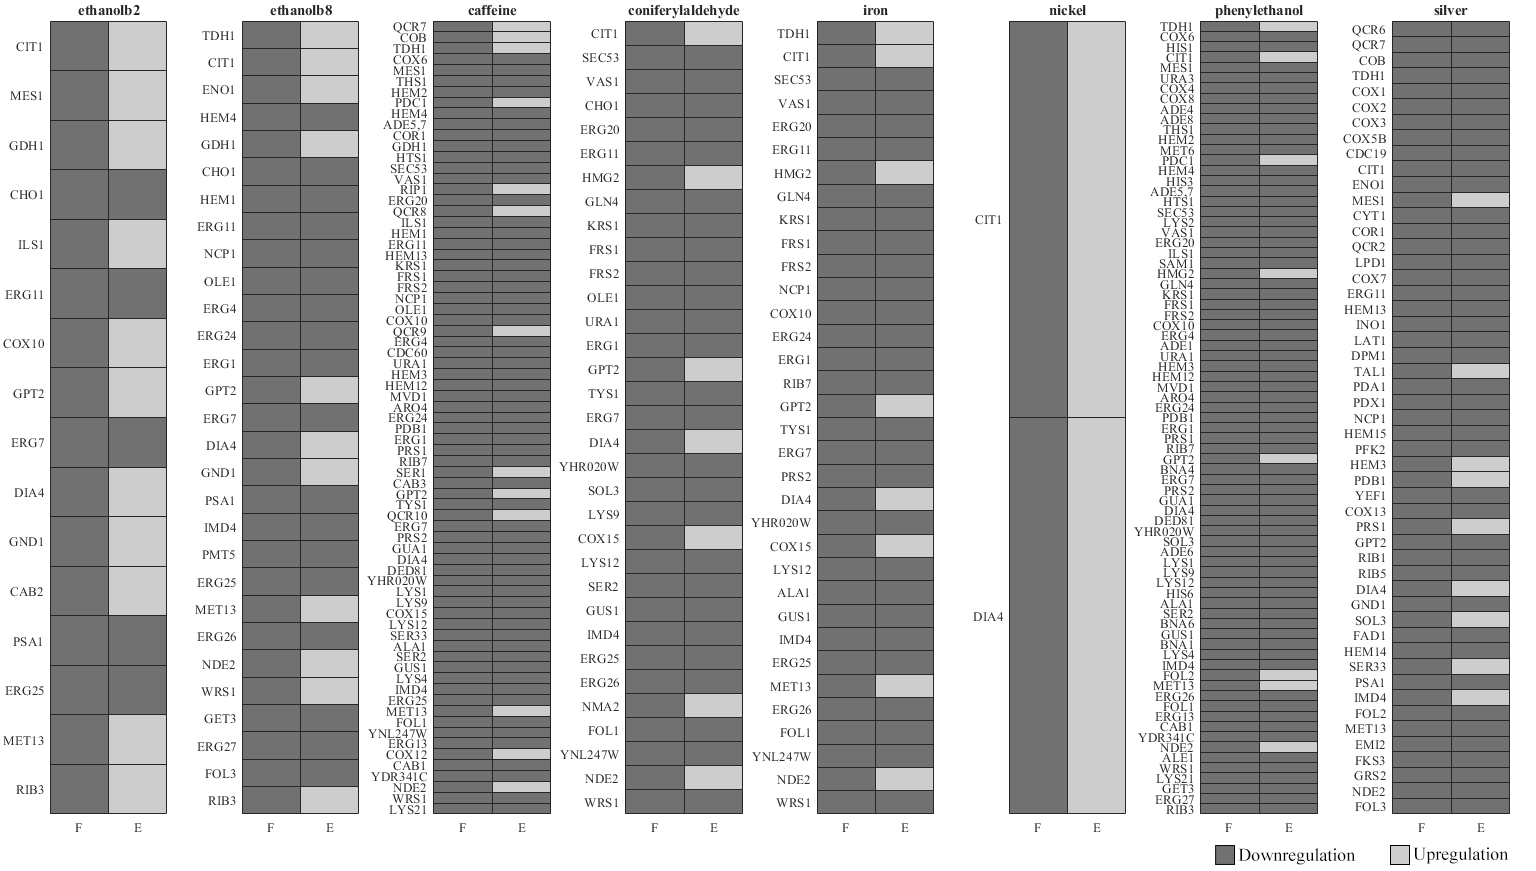
\includegraphics[width=1\columnwidth]{figures/sampling_regulation_heatmaps.png}
  \caption[Regulation of the enzymes obtained from the random sampling of solution spaces (F) and differential expression analysis (E) in all models. Enzymes that only have significant (p$<$0.05) changes are plotted in both flux and expression changes]{Regulation of the enzymes obtained from the random sampling of solution spaces (F) and differential expression analysis (E) in all models. Enzymes that only have significant (p$<$0.05) changes are plotted in both flux and expression changes. }
  \label{fig:sampling_regulation_heatmaps}
  \end{center}
\end{figure}
